% A LaTeX template for MSc Thesis submissions to 
% Politecnico di Milano (PoliMi) - School of Industrial and Information Engineering
%
% S. Bonetti, A. Gruttadauria, G. Mescolini, A. Zingaro
% e-mail: template-tesi-ingind@polimi.it
%
% Last Revision: October 2021
%
% Copyright 2021 Politecnico di Milano, Italy. NC-BY

\documentclass{Configuration_Files/PoliMi3i_thesis}

%------------------------------------------------------------------------------
%	REQUIRED PACKAGES AND  CONFIGURATIONS
%------------------------------------------------------------------------------

% CONFIGURATIONS
\usepackage{parskip} % For paragraph layout
\usepackage{setspace} % For using single or double spacing
\usepackage{emptypage} % To insert empty pages
\usepackage{multicol} % To write in multiple columns (executive summary)
\setlength\columnsep{15pt} % Column separation in executive summary
\setlength\parindent{0pt} % Indentation
\raggedbottom  

% PACKAGES FOR TITLES
\usepackage{titlesec}
% \titlespacing{\section}{left spacing}{before spacing}{after spacing}
\titlespacing{\section}{0pt}{3.3ex}{2ex}
\titlespacing{\subsection}{0pt}{3.3ex}{1.65ex}
\titlespacing{\subsubsection}{0pt}{3.3ex}{1ex}
\usepackage{color}

% PACKAGES FOR LANGUAGE AND FONT
\usepackage[english]{babel} % The document is in English  
\usepackage[utf8]{inputenc} % UTF8 encoding
\usepackage[T1]{fontenc} % Font encoding
\usepackage[11pt]{moresize} % Big fonts

% PACKAGES FOR IMAGES
\usepackage{graphicx}
\usepackage{transparent} % Enables transparent images
\usepackage{eso-pic} % For the background picture on the title page
\usepackage{subfig} % Numbered and caption subfigures using \subfloat.
\usepackage{tikz} % A package for high-quality hand-made figures.
\usetikzlibrary{}
\graphicspath{{./Images/}} % Directory of the images
\usepackage{caption} % Coloured captions
%\usepackage[dvipsnames]{xcolor} % Coloured captions
\usepackage{xcolor} % Coloured captions
\usepackage{amsthm,thmtools,xcolor} % Coloured "Theorem"
%\usepackage{amsthm,thmtools} % Coloured "Theorem"
\usepackage{float}

% STANDARD MATH PACKAGES
\usepackage{amsmath}
\usepackage{amsthm}
\usepackage{amssymb}
\usepackage{amsfonts}
\usepackage{bm}
\usepackage[overload]{empheq} % For braced-style systems of equations.
\usepackage{fix-cm} % To override original LaTeX restrictions on sizes

% PACKAGES FOR TABLES
\usepackage{xltabular}
\usepackage{longtable} % Tables that can span several pages
\usepackage{colortbl}

% PACKAGES FOR ALGORITHMS (PSEUDO-CODE)
\usepackage{algorithm}
\usepackage{algorithmic}

% PACKAGES FOR REFERENCES & BIBLIOGRAPHY
\usepackage[colorlinks=true,linkcolor=black,anchorcolor=black,citecolor=black,filecolor=black,menucolor=black,runcolor=black,urlcolor=black]{hyperref} % Adds clickable links at references
\usepackage{cleveref}
\usepackage[square, numbers, sort&compress]{natbib} % Square brackets, citing references with numbers, citations sorted by appearance in the text and compressed
\bibliographystyle{abbrvnat} % You may use a different style adapted to your field

% OTHER PACKAGES
\usepackage{pdfpages} % To include a pdf file
\usepackage{afterpage}
\usepackage{lipsum} % DUMMY PACKAGE
\usepackage{fancyhdr} % For the headers
\fancyhf{}

% -----------
\usepackage{enumitem}
\usepackage{listings}
\usepackage{alloy-style}
\usepackage{xltabular}

% Input of configuration file. Do not change config.tex file unless you really know what you are doing. 
% Define blue color typical of polimi
\definecolor{bluepoli}{cmyk}{0.4,0.1,0,0.4}

% Custom theorem environments
\declaretheoremstyle[
  headfont=\color{bluepoli}\normalfont\bfseries,
  bodyfont=\color{black}\normalfont\itshape,
]{colored}

% Set-up caption colors
\captionsetup[figure]{labelfont={color=bluepoli}} % Set colour of the captions
\captionsetup[table]{labelfont={color=bluepoli}} % Set colour of the captions
\captionsetup[algorithm]{labelfont={color=bluepoli}} % Set colour of the captions

\theoremstyle{colored}
\newtheorem{theorem}{Theorem}[chapter]
\newtheorem{proposition}{Proposition}[chapter]

% Enhances the features of the standard "table" and "tabular" environments.
\newcommand\T{\rule{0pt}{2.6ex}}
\newcommand\B{\rule[-1.2ex]{0pt}{0pt}}

% Pseudo-code algorithm descriptions.
\newcounter{algsubstate}
\renewcommand{\thealgsubstate}{\alph{algsubstate}}
\newenvironment{algsubstates}
  {\setcounter{algsubstate}{0}%
   \renewcommand{\STATE}{%
     \stepcounter{algsubstate}%
     \Statex {\small\thealgsubstate:}\space}}
  {}

% New font size
\newcommand\numfontsize{\@setfontsize\Huge{200}{60}}

% Title format: chapter
\titleformat{\chapter}[hang]{
\fontsize{50}{20}\selectfont\bfseries\filright}{\textcolor{bluepoli} \thechapter\hsp\hspace{2mm}\textcolor{bluepoli}{|   }\hsp}{0pt}{\huge\bfseries \textcolor{bluepoli}
}

% Title format: section
\titleformat{\section}
{\color{bluepoli}\normalfont\Large\bfseries}
{\color{bluepoli}\thesection.}{1em}{}

% Title format: subsection
\titleformat{\subsection}
{\color{bluepoli}\normalfont\large\bfseries}
{\color{bluepoli}\thesubsection.}{1em}{}

% Title format: subsubsection
\titleformat{\subsubsection}
{\color{bluepoli}\normalfont\large\bfseries}
{\color{bluepoli}\thesubsubsection.}{1em}{}

% Shortening for setting no horizontal-spacing
\newcommand{\hsp}{\hspace{0pt}}

\makeatletter
% Renewcommand: cleardoublepage including the background pic
\renewcommand*\cleardoublepage{%
  \clearpage\if@twoside\ifodd\c@page\else
  \null
  \AddToShipoutPicture*{\BackgroundPic}
  \thispagestyle{empty}%
  \newpage
  \if@twocolumn\hbox{}\newpage\fi\fi\fi}
\makeatother

%For correctly numbering algorithms
\numberwithin{algorithm}{chapter}

%----------------------------------------------------------------------------
%	NEW COMMANDS DEFINED
%----------------------------------------------------------------------------

% EXAMPLES OF NEW COMMANDS
\newcommand{\bea}{\begin{eqnarray}} % Shortcut for equation arrays
\newcommand{\eea}{\end{eqnarray}}
\newcommand{\e}[1]{\times 10^{#1}}  % Powers of 10 notation

%----------------------------------------------------------------------------
%	ADD YOUR PACKAGES (be careful of package interaction)
%----------------------------------------------------------------------------

%----------------------------------------------------------------------------
%	ADD YOUR DEFINITIONS AND COMMANDS (be careful of existing commands)
%----------------------------------------------------------------------------

%----------------------------------------------------------------------------
%	BEGIN OF YOUR DOCUMENT
%----------------------------------------------------------------------------

\begin{document}

\fancypagestyle{plain}{%
\fancyhf{} % Clear all header and footer fields
\fancyhead[RO,RE]{\thepage} %RO=right odd, RE=right even
\renewcommand{\headrulewidth}{0pt}
\renewcommand{\footrulewidth}{0pt}}

%----------------------------------------------------------------------------
%	TITLE PAGE
%----------------------------------------------------------------------------

\pagestyle{empty} % No page numbers
\frontmatter % Use roman page numbering style (i, ii, iii, iv...) for the preamble pages

\puttitle{
	title=RASD: Requirements Analysis and Specification Document,
	name1=Lorenzo Ferretti, % Author Name and Surname
	name2=Lorenzo Manoni, 
	name3=Carlo Sgaravatti,
	academicyear=2022-2023,
        version=1.0,
	date=23/12/2022
} % These info will be put into your Title page 

%----------------------------------------------------------------------------
%	PREAMBLE PAGES: ABSTRACT (inglese e italiano), EXECUTIVE SUMMARY
%----------------------------------------------------------------------------
\startpreamble
\setcounter{page}{1} % Set page counter to 1

%----------------------------------------------------------------------------
%	LIST OF CONTENTS/FIGURES/TABLES/SYMBOLS
%----------------------------------------------------------------------------

% TABLE OF CONTENTS
\thispagestyle{empty}
\tableofcontents % Table of contents 
\thispagestyle{empty}
\cleardoublepage

%-------------------------------------------------------------------------
%	THESIS MAIN TEXT
%-------------------------------------------------------------------------
% In the main text of your thesis you can write the chapters in two different ways:
%
%(1) As presented in this template you can write:
%    \chapter{Title of the chapter}
%    *body of the chapter*
%
%(2) You can write your chapter in a separated .tex file and then include it in the main file with the following command:
%    \chapter{Title of the chapter}
%    \input{chapter_file.tex}
%
% Especially for long thesis, we recommend you the second option.

\addtocontents{toc}{\vspace{2em}} % Add a gap in the Contents, for aesthetics
\mainmatter % Begin numeric (1,2,3...) page numbering

\chapter{Introduction}

\section{Purpose}

The scope of this document consists of showing the requirements of the system to be. Since the system to be is made up of two different sub-systems the eMSP and the CPMS, that also have different final users, this document will include a description of both systems.
Characteristics of the system are described following a top-down approach with the aim to facilitate comprehension of the readers.


\subsection{Goals}
User goals:
\begin{enumerate}[label=\textbf{G\arabic*}]

    \item Allow users to visualize nearby charging stations and the relative price of energy, socket availability, and if they provide offers;
    
    \item Allow users to reserve a charge at a certain charging point for a certain time slot;
    
    \item Allow the user to start a charging process at a station;

    \item Allow the user to monitor the status of the charging process with valuable data;

    \item Allow the user to pay for the service;

    \item Gives users suggestions about the optimal schedule to charge the vehicle depending on battery status, the schedule of the users, and offers provided by CPOs;

\end{enumerate}

CPO goals:
\begin{enumerate}[label=\textbf{G\arabic*}]\setcounter{enumi}{6}

    \item Allow CPOs dynamically decide from which DSO to acquire energy providing information on energy prices;

    \item Allow CPOs dynamically decide the cost of charging and when setting special offers;

    \item Allow CPOs dynamically decide whether or not to store energy in their internal batteries;

    \item Allow CPOs dynamically decide, during a charging process, to use the stored energy in the battery or to acquire directly from DSOs to fulfil the charge or a mix of both;

    \item Allow the CPOs to Manage their CPs and the relative socket in order to enable drivers to use them.

\end{enumerate}

\section{Scope}
Recent technological advances make electric vehicles (EVs) a plausible alternative to gasoline vehicles and give them the potential to enable zero or low-emission transportation. Improved batteries are cheaper and permit longer driving ranges making EVs more attractive to consumers than in the past.
Achieving zero emissions is a goal shared by multiple countries and new green technologies are encouraged all around the world. Investments in  Green transition energy projects are estimated to value 257 billion dollars. 

Considering that the Charging Point infrastructure is a crucial asset to succeed in the EV strategy, our product aims to optimally manage the complex infrastructure needed for electric mobility. 
The scope of the project aims to satisfy both driver  and Charging Point Operators needs.
Drivers need new means to feel comfortable with Electric Mobility, "range out anxiety" has been defined as one of the main issues that obstacle to the adoption of Electric Vehicles in many parts of the world.
One of our major goals is to improve EV' drivers' experience through a mobile application, the eMSP, that can help drivers to feel more comfortable, empowering users by informing them about all the charging points they can access and allowing them to reserve charging sessions at a Charging Point. To improve drivers' experience the system actively makes suggestions of stops during a trip using the navigation system and is able to access users' calendars to prone charging sessions that fit the user schedule at best.
The system assists the driver also during the charging sessions, providing information on the charging process and notifying it when the process is complete. The user can also benefit from our payment system to pay in a rapid and smart way to pay.

This is not the only aspect of the EV infrastructure that we care about, in fact, the system also provides software for the management of the CP. This software is the CPMS and the scope of this product is to help the Charging Point Operators (CPOs) to manage their Charging Points. We provided all crucial functionality for all operations executed by them. We support the acquisition of energy by different energy providers (DSOs), we provide a system to manage each Charging Point allowing the CPOs to monitor the status of each socket, and the status of the battery if present and to perform all critical operations on them (like the exclusion of the battery from the system, the management of the stock availability and the socket charging profile). 
Our system doesn't limit to offering industry-standard operations, in fact, it has an intelligent component for optimizing energy acquisition and management. This is a crucial feature that enables CPOs to reduce costs through a cost-optimal energy choice, which can result to be a really important asset in a competitive scenario. 
Another key feature of the system is to give to CPOs the possibility to create special offers to the customer that can directly access them through the eMSP. 

Both the eMSP and the CPMS can interact with all the other systems provided by others.
\subsection{World Phenomenas}

\begin{enumerate}[label=\textbf{WP\arabic*}]
    \item The user arrives at the CP with his electric car;
    \item The user sets a route in the navigation system;
    \item The user uses a calendar to organize a personal schedule;
    \item The user plugs the socket;
    \item The user unplugs the socket.
    \item The user drives his electric car.
    \item The CP locks a socket.
    \item The CP unlocks a socket.
    \item The CP starts the energy flow to the connected vehicle.
    \item The CP stops the energy flow to the connected vehicle.
\end{enumerate}

\subsection{Shared Phenomenas}

\begin{table}[H]
\centering 
    \begin{xltabular}{\textwidth}{| >{\columncolor{bluepoli!40}}p{3em}|X|c|}
    \hline
    \rowcolor{bluepoli!40}
     & \textbf{Phenomena} & \textbf{Controller}\T\B \\
    \hline \hline
    \textbf{SP1} & The user registers to the eMSP & W\T\B\\
    \hline
    \textbf{SP2} & The user logins to the eMSP & W\T\B\\
    \hline
    \textbf{SP3} & The user checks the CP nearby & W\T\B\\
    \hline
    \textbf{SP4} & The user checks for the offers & W\B\\
    \hline
    \textbf{SP5} & The user reserves a CP & W\B\\
    \hline
    \textbf{SP6} & The user checks the status of the charging process & W\B\\
    \hline
    \textbf{SP7} & The user stop the charging process & W\B\\
    \hline
    
    \textbf{SP8} & The user ends the charging process & W\B\\
    \hline
    \textbf{SP9} & The user pays for the service & W\B\\
    \hline
    \textbf{SP10} & The user checks for the offers & W\B\\
    \hline
    \textbf{SP11} & The CPO selects the source of energy & W\B\\
    \hline
    \textbf{SP12} & The CPO manages the offers & W\B\\
    \hline
    \textbf{SP13} & The CPO register a new CP in the CPMS & W\B\\
    \hline
    \textbf{SP14} & The CPMS detects a plugged socket through the CP & W\B\\
    \hline
    \textbf{SP15} & The CPMS detects a unplugged socket through the CP & W\B\\
    \hline
    \textbf{SP16} & The eMSP notifies the user when the charging process is completed & M\B\\
    \hline
    \textbf{SP17} & The eMSP retrieves information from the user's calendar & M\B\\
    \hline
    \textbf{SP18} & The eMSP retrieves information from the user navigation system & M\B\\
    \hline
    \textbf{SP19} & The eMSP retrieves information from the car battery & M\B\\
    \hline
    \textbf{SP20} & The eMSP notifies the user of suggestions for the recharging process at a certain CP and time frame & M\B\\
    \hline
    \textbf{SP21} & The CPMS communicates to the CP to lock/unlock a socket & M\B\\
    \hline
    \textbf{SP22} & The CPMS communicates to the CP to start/end the charging process & M\B\\
    \hline
    \textbf{SP23} & The CPMS acquires information about the CPs (socket status, battery status, position, charging processes) & M\B\\
    \hline
    \textbf{SP24} & The CPMS acquires information about energy prices and availability from DSOs & M\B\\
    \hline
    \textbf{SP25} & The CPMS changes the source of energy to recharge vehicles & M\B\\
    \hline
    \textbf{SP26} & The CPMS communicates to the CP to store the energy in the battery & M\B\\
    \hline
    \end{xltabular}
    \caption{Shared Phenomena}
\end{table}

\section{Glossary}

\subsection{Definitions}

\begin{itemize}
    \item \textbf{Charging Point:} it's the physical system where an electric vehicle can be recharged.
    \item \textbf{Charging Point Operator:} it's a company that owns some charging points.
    \item \textbf{Distribution System Operator:} it's a company that provides energy to the charging points.
    \item \textbf{Socket:} it's a physical connector of the charging point on which a vehicle is connected when recharging. There are three types of physical connection for the sockets: slow, fast and rapid. Each of those types specifies a maximum value of energy flow that the socket is able to provide to the connected vehicles.
    \item \textbf{Charging Profile:} it's a schedule that defines how much energy a particular socket will provide to the connected vehicle during the charging process. Usually, the schedule is composed of a list of different periods (e.g. different time intervals of a day) on which the amount of energy that the socket will provide can be different.
    \item \textbf{User:} it's a person who is registered to the service and that can make reservations in some charging points in order to recharge his vehicle.
    \item \textbf{Charging Session:} it's the process by which a vehicle is being recharged by a certain socket.
    \item \textbf{Notification:} it's an alert that the eMSP sends to the user to inform him of a certain event.
    \item \textbf{Tariff:} it's the price, specified in terms of units of energy, for recharging the vehicles in a certain charging point. Different types of sockets of the same charging point can have different tariffs.
    \item \textbf{Special Offer:} it's a particular tariff that is valid only for a certain time slot.
    \item \textbf{Current Energy Source:} it's a source of energy that is providing energy to a charging point for recharging vehicles. A charging point can have more than one current energy source, i.e. a DSO and one or more batteries.
    \item \textbf{Energy Mix:} it's the way in which the charging point is using its current energy sources. Given the amount of energy demanded, the Energy mix specifies the relative percentage of energy that the charging point should try to satisfy using the battery/batteries.
    \item \textbf{Manual/Automatic mode:} the way in which the CPMS is used to manage a charging point. There are three functions that can have one of the two modalities: the DSO selection, the energy mix management and the tariff policy management. If the CPMS is in automatic mode for a certain charging point and for a certain function, it automatically optimizes that function without the need for manual intervention. In manual mode, the CPMS allow the CPO to manually manage the configurations.
    \item \textbf{Battery level:} it's the actual amount of energy stored inside a battery of a charging point.
    \item \textbf{Battery Minimum Energy Trigger:} it’s a value that indicates the minimum battery level at which the battery can be used as an energy source. When the CPMS is set on manual mode for energy management and a battery reaches that value the CPMS automatically uses another energy source to recharge it.
    \item \textbf{Battery Maximum Energy Trigger:} it’s a value that indicates the maximum battery level at which the battery can be used as an energy source. When the CPMS is set on manual mode for energy management and a battery reaches that value the CPMS automatically uses the battery to recharge the plugged cars. This value must be higher or equal to the Minimum Energy trigger.
    \item \textbf{Battery availability:} a battery can be available or unavailable. Only in the first case, it can be used as an energy source for the charging point.
    \item \textbf{Battery status:} identifies how the battery is working at a given time when it is available. The battery can have the following status:
        \begin{itemize}
            \item Export: the battery is used as an energy source for the charging point.
            \item Import: the battery is being recharged by another energy source, i.e. a DSO.
            \item Idle: the battery isn't used as an energy source and isn't being recharged.
        \end{itemize}
    %\item \textbf{Minimum Energy Request:}
\end{itemize}

\subsection{Acronyms}

\begin{itemize}
    \item \textbf{CPMS:} Charging Point Management System
    \item \textbf{eMSP:} e-Mobility Service Provider
    \item \textbf{OCPI:} Open Charge Point Interface, which is the communication protocol used to connect eMSP and CPMS.
    \item \textbf{OCPP:} Open Charge Point Protocol, which is the communication protocol used to connect the CPMS and the charging point.
    \item \textbf{API:} Application Programming Interface, it's a way by which two software systems communicate.
\end{itemize}

\subsection{Abbreviations}

\begin{itemize}
    \item \textbf{CP:} Charging Point
    \item \textbf{CPO:} Charging Point Operator
    \item \textbf{DSO:} Distribution System Operator
    \item \textbf{Gn:} Goal number n
    \item \textbf{WPn:} World Phenomena number n
    \item \textbf{SPn:} Shared Phenomena number n
    \item \textbf{Dn:} Domain assumption number n
    \item \textbf{UCn:} Use Case number n
    \item \textbf{Rn:} Requirement number n
    
\end{itemize}

\section{Revision history}

\begin{itemize}
    \item December 23, 2022: version 1.0 (first release)
\end{itemize}

\section{Reference Documents}
\begin{itemize}
    \item Project assignment ad specification document "Assignment RDD AY 2022-2023\_v3.pdf"
    \item OSCP 2.0 Specification.pdf
    \item SMUD OpenADR Implementation Design Guide v1\_0.pdf
    \item ocpp-1.6.pdf
    \item OCPI-2.2.1.pdf
\end{itemize}

\section{Document Structure}
The document’s structure is designed with the aim to introduce gradually the reader into the system leading to an increased detail level, for this reason, it has been decided to follow a top-down approach in the description of the problem and requirements. 
After the first chapter of the introduction, an entire section is dedicated to the introduction of the problem. 

The aim of that section consists in to give the reader a general perspective of the product in question(section 2.1) providing a description of the domain through a class diagram, and a state diagram and describing the main different scenarios. But also provides a high-level perspective of the system’s functionality (section 2.2) through the product functions description, a description of the different users that will interact with the system (section 2.3), and the assumption taken to model and design the system  (section 2.4).


The third section is dedicated to providing a more detailed description of the requirements.
First (section 3.1) are described the External Interface Requirements that include the Hardware, Software, Communication, and User interface. 
Then an entire section  (section 3.2) is dedicated to the functional requirements including a detailed description of all use cases, to better help the reader’s understanding, each use case comes with a sequence diagram. 
Then (section 3.3) the performance requirements are described.  
Section 3.4  is about the design constraint of the system, which describes the Standard Compliance and the Hardware Limitations. 
The last part (section 3.5) is dedicated to the Software System Attributes, there is described the desired performance that the system should satisfy in terms of Reliability, Availability, Security, Maintainability, and Portability. Each one of these aspects has exposed the criticality of it for the success of the application.

The fourth section is entirely dedicated to the formal analysis of the requirements using alloy, in order to validate their completeness and consistency of them. 

Then the last two sections describe the effort spent by the team to model the requirements and write the document and the last one included all the references consulted to write the document. 
\chapter{Overall Description}

\section{Product perspective}

\subsection{Scenarios}

\begin{enumerate}
    \item \textbf{A new user wants to start using the eMall service.} 
    The user Luke has just bought his new electric vehicle and wants to find places where he can charge the battery of his new car. Luke decides to download the eMall service on his mobile phone and register for it. He opens the applications and inserts his data, including his car information and a payment method; he also allows the system to access his calendar, his position, and navigation system in order to use all features provided.

    \item \textbf{A user inserts his vehicle's information.} 
    John is a new user really passionate about electric cars, in his garage has 4 different electric vehicles. During the registration, he inserts all his cars, provides the related information, and selects the car that uses on a daily basis as his "Favourite Vehicle". The eMSP gives John suggestions considering his "Favourite Vehicle", also when John books a charge, the system considers only the sockets compatible with the car. On the weekend John decides to drive another car and selects his truck as his "Favourite Vehicle".

    \item \textbf{A user receives a suggestion based on the navigation system.} \newline
    The user Luke is driving for a long trip and his navigation system is active. While he is following the path, the system acquires information on the battery status and realizes that he will not be able to reach the destination without stopping for charging and it computes the best charging station to stop. The system sends a notification to Luke about the suggested stop for the "Favourite Vehicle"; Luke accepts the suggestion and the system reserve a socket of the correct type for his car in the suggested charging point on the path of the navigation system.

    \item \textbf{User recharges his vehicle and pays for the service.} \newline
    Luke has already booked a charge in the charging station Y, arrives at the location, and parks the car in front of the correct socket. From the mobile application, he selects the option to unlock the socket. The CPMS unlocks the socket, Luke inserts the plug in the socket and clicks on the start charging process option. The CPMS locks the socket and considers all available options to transfer the energy considering the cost of the electricity of every DSO available and the CP battery, at the end it decides to use the CP battery for the energy flow and starts the charging process. After some minutes the CP detects that the battery of the car is full and stops the energy flow sending an update to the CPMS. The CPMS informs the eMSP that sends a notification to Luke, who returns to the car. Luke ends the charging process with his mobile application, the CPMS unlocks the socket and Luke removes the plug. In the end, the eMSP pays for the service with the payment method provided by Luke. Now the socket is free and available for other users.

    \item \textbf{CPO chooses a DSO as the energy source for a CP.} \newline
    Mark works for a CPO, recently the company signed a contract with "Energy Distribution" DSO that force the company to acquire the energy only from it for an entire month. Mark login into the CPMS of the company with his credentials and select the option that forces every CP to acquire energy only from "Energy Distribution". At the end of the month, Mark reset the CMPS to let it choose the best strategy to acquire energy.

    \item \textbf{CPO includes the battery as an energy source for a CP.} \newline
    Mark, that still works for a CPO, through the CPMS must do some maintenance work for increasing the CP battery capacity, so decides to manually set the energy acquisition only from DSOs, excluding the CP battery. After a week the CP battery is repaired and Mark resets the default settings, in this way the CPMS has full control of the CP. The CPMS notices that the prices of the DSO are increased exponentially in this period and the CP battery is not used to its new full potential, so mix the energy flow with the DSOs, in order to optimize the cost.

    \item \textbf{User receives a suggestion based on the calendar.} \newline
    Luke uses his calendar on a daily basis to manage his business meetings. The eMSP acquires information from his mobile phone calendar application, considers also the battery status, and realizes that there is a convenient CP near the business meeting location 30 minutes before it. It sends a notification to Luke who accepts the suggestion and a socket of his "Favourite Vehicle" type is booked in that CP.
\end{enumerate}

\subsection{Class Diagram}
The Class Diagram describes our entire system, composed of eMSP and CPMS. The most important entities described in the diagram are:
\begin{description}
    \item [User:] It represents the user of the eMSP, it has a username, an email, and a password;
    
    \item[Vehicle:] Is a vehicle registered by one or more users through a VehicleAPI that verifies the VIN, used as a unique id. The user can set a vehicle as the favourite vehicle for filtering the sockets during StationResearch, and receiving ChargingSuggestion Notifications based on the VehicleBattery and the type of socket supported by the vehicle;
    
    \item [StationResearch:] Is based on a Position made by latitude and longitude and a distance range in a certain time frame in order to retrieve the Charging Points in that area;
    
    \item [Reservation:] Is made by a user on a specific Socket in a certain time frame at the related tariff or special offer;
    
    \item [ChargingSession:] Is related to a Reservation and is described by the amount of energy consumed, the actual battery status of the connected car, the duration of the recharge, and a boolean that recognizes a finished session. When the battery status is full, a ChargingEndedNotification is sent to the user;

    \item [Payment:] represents a payment, related to a user and a charging session: This class include both successful payments and pending ones if the payment wasn't able to be concluded.
    
    \item [ChargingPoint:] It represents a real Charging Point, owned by a CPO. It has a Position (latitude and longitude), different Sockets of different types, having its own status. Each CP has a Tariff for each socket type and could have a SpecialOffers;
    
    \item [EnergySource:] It represents an energy source related to a certain CP. It can be a DSOEnergySource, representing a DSO, or a ChargingPointBattery representing a battery connected to the CP. "CurrentEnergySource" is the relation that identifies the resources  that can be used at a given time. 
\end{description}

\begin{figure}[H]
    \centering
    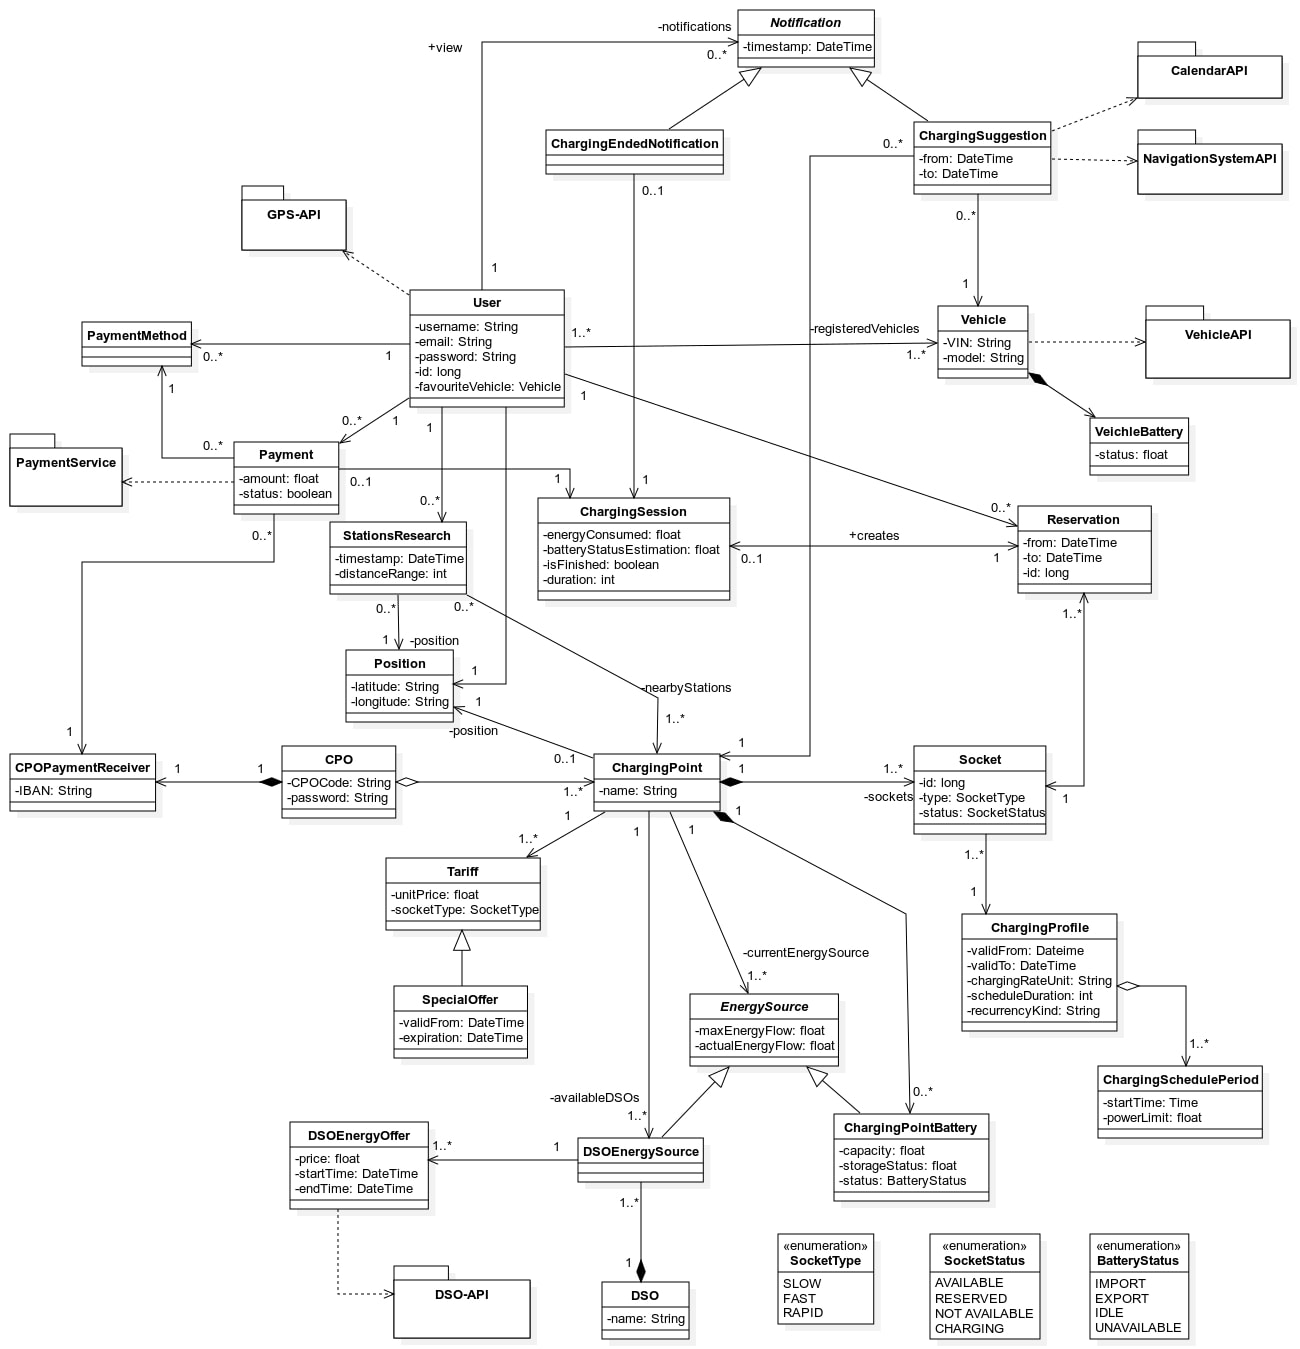
\includegraphics[width=1\textwidth]{Images/ClassDiagram.jpg}
    \caption{Class Diagram}
\end{figure}

\subsection{State Diagrams}
The following diagrams describe the states that some of the most important entities can assume.\\

The \textbf{Reservation} has four different states. The first one is triggered when a new reservation is created that sets it in the RESERVED state. When the expiration time is passed or the user cancels the reservation will change its state to CANCELLED, ending the process. If the user doesn't cancel the reservation and it is still valid, it can enter into the CHARGING state until the charging session is over, this will bring to the state COMPLETED, ending the process.
\begin{figure}[H]
    \centering
    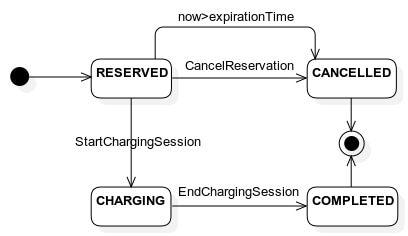
\includegraphics[width=0.6\textwidth]{Images/StateDiagrams/Reservation.jpg}
    \caption{Reservation}
\end{figure}

Each \textbf{Charging Session} can take four states. The entry state is the CHARGING one triggered when the user starts the charging session. From this state, we can reach the INVALID state which is useful when an error occurs and we want to avoid billing the user, and the STOPPED state when the user reaches a full charge or wants to stop the charging before it. By the latter, removing the socket from the CP, we enter the ENDED state.
\begin{figure}[H]
    \centering
    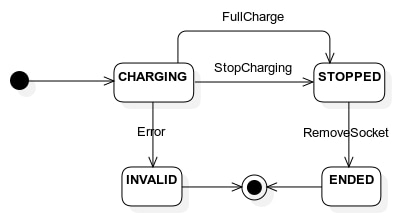
\includegraphics[width=0.6\textwidth]{Images/StateDiagrams/Charging Session.jpg}
    \caption{Charging Session}
\end{figure}

The \textbf{Sockets} beginning state is the AVAILABLE one, when a socket is reserved it changes its state to RESERVED and can return to AVAILABLE when a reservation is canceled. The CHARGING state can be reached when a charging session is started and returns to AVAILABLE when it's ended.
These three states can reach the unavailable state that is set when an error occurs, from this state we can remove the socket entering the REMOVED state or return to the AVAILABLE one.
\begin{figure}[H]
    \centering
    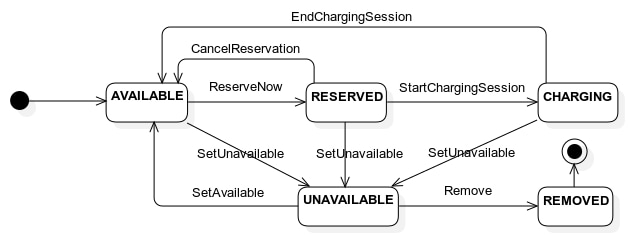
\includegraphics[width=0.9\textwidth]{Images/StateDiagrams/Socket.jpg}
    \caption{Socket}
\end{figure}


The \textbf{Charging Station Battery} has four states. The main state is the IDLE one, which can reach the other three states. When the battery is storing energy it enters the IMPORT state and returns to IDLE when it stops storing or if it is full. When the battery is used as an energy source for a charging point, it enters the EXPORT state and returns to IDLE when it stops charging other vehicles or if it is empty. The last state is UNAVAILABLE which is triggered when an error occurs, from this the battery can return to IDLE or be removed.
\begin{figure}[H]
    \centering
    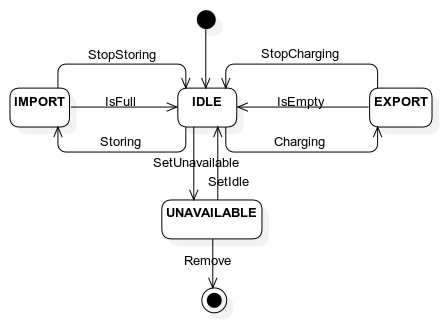
\includegraphics[width=0.7\textwidth]{Images/StateDiagrams/Charging Station Battery.jpg}
    \caption{Charging Station Battery}
\end{figure}

\section{Product functions}

\subsection{eMSP Product Functions}
\begin{enumerate}
     \item \textbf{Search and Reservation of a CP.} \newline
    One of the main goals of the eMSP is to allow the User to search the CP around it and reserve a socket if it's free. In order to perform these operations the eMSP needs to have a map view that by default is centered on the User's position and enables it to look at the CP around. Of course, a User can be interested in searching for a CP near a position that has nothing to do with his current position. For this reason, the eMSP has to provide also a way to insert another location and look for the CPs near the position selected. Another important aspect to consider is that the user might be interested in researching a CP that has a free socket or that has a compatible socket with his vehicle.
    The User should have the possibility to insert vehicle information into the application and the system can use the user’s favourite vehicle to filter the results on the map.
    In order to achieve maximum flexibility we designed the system in a way that after the research of a CP, all kinds of CPs are displayed (even the ones that have all the sockets currently busy or incompatible), but they will be shown to the user in different ways depending on which of these three categories they belong: 
    \begin{enumerate}
        \item The CP has one or more sockets that are compatible and currently available. The user is very interested in these CPs since are the ones where he can reserve a socket compatible with his favourite vehicle;
        \item The CP has one or more sockets that are compatible with his favourite vehicle, but they are all busy. The user can be interested in this kind of CP since he may be interested in waiting until a socket is free;
        \item The CP has all sockets that are not compatible with the user’s favourite vehicle. This case can be useful for users that have multiple vehicles.
    \end{enumerate}
    
    The user of course can reserve a free socket for a charging session. The reservation process requires that the user has no pending payments. When a reservation is made the User has 20 minutes to go to the CP and start the charging process. 
    The User can also delete a reservation if has changed his mind, while if he doesn’t start the charging process within 20 minutes the reservation will expire. The system is designed in a way that each user can have at most one reservation active at a time. \newline
   
    \item \textbf{Charging session and payment.} \newline
    Another fundamental functionality offered by the eMSP is the possibility to start a recharge, monitor it, and pay for the service. 
    The user in eMSP has to reserve a socket before starting the charging process. So when the drivers arrive at the CP can open the eMSP application and select the "start charging process" option, at this point, the CP’s socket connector is unlocked and the user can insert the socket from his car into the CP’s connector. The CP is able to detect that a car is plugged in and can start the energy transfer while locking the socket. During the charging process, the eMSP gives the user the possibility to observe the charging process and the information about his vehicle’s battery. The CP blocks the charging process in an automatic way the battery is full and in this case the eMSP notifies the user through a pop-up notification that the process is completed. The system gives also the user the possibility to stop a charging process when he wants before the battery of his vehicle is full.
    After a charging process is stopped the user can unlock the socket; the charging session is ended now. The system at this point asks the user to pay for the charging process. When the user allows the eMSP to process the payment, the eMSP use the payment method selected by the user to pay through an external payment service. If the payment fails, it will be marked as unsolved. The system will prevent the user with an unsolved payment to make new reservations and will give them the possibility to pay at a later time.
    The system notifies the user of the payment's success or failure.\newline
   
    \item \textbf{Suggestions.} \newline
    A very important part that characterizes our eMSP is the feature of making suggestions to the user and proposing a socket to reserve. 
    When a user logs in for the first time into the eMSP, the eMSP will ask it permission to access his calendar and navigation system to retrieve information to optimize suggestions. The eMSP will interact with these two applications of the user but also with an external API that retrieves the battery status of the favourite vehicle. The eMSP will make a suggestion when the vehicle battery reaches a certain percentage. When this happens the eMSP will interact at first with the navigation system to retrieve the navigation path if inserted. In this case will compute the best stop option to minimize the price of the recharge and the user's time cost to reach the CP and complete the recharge, considering the information of his favourite vehicle and the status of the socket of each CPs under a certain range. 
    Then the system will interact with the calendar system in order to understand if the user has an appointment schedule during the day and acquire the relative location. 
    The eMSP will combine all this information to make a suggestion. 
    If the calendar and navigation system do not give relevant information about the user the system will use user’s the current position to make a suggestion.
    The user will receive the suggestion in form of a pop-up notification and can accept or decline it. When a suggestion is accepted the system will reserve the relative socket. If an error occurs during this process, the eMPS will recompute another suggestion for the User. 
\end{enumerate}

\subsection{CPMS product functions}

\begin{enumerate}
    \item \textbf{Manage energy source.} \newline
    The CPMS offers the CPO several functionalities, one of the most important is the energy source acquisition system. 
    The CPMS is designed in a way that is able to minimize the cost that the CPO has to bear to provide energy to the CPs. 
    For this purpose, the CMPS has two different “abilities” that combined enable the system to behave in the optimal way to achieve cost efficiency. 

    Firstly the system is able to select from which DSO acquires energy in an optimal way, making the choice in a different way for each CP managed, considering the expected traffic, energy prices, and DSO’s availability and offers for each CP. 

    Another point is to exploit the battery usage for each CP at its best, computing the optimal strategy to schedule the energy acquisition period vs exploiting the battery.

    These two aspects combined let the CPMS be maximum efficient. By the way, the CPMS allows the CPOs to control directly both aspects (Manual Mode). In fact, the CPO can manually select from which DSO acquires energy and how to use the battery for each CP. In addition, the CPO can select the Manual Mode for one of the two functionalities and let the CPMS automatically optimise the other one. For example, the CPO can force the selection of the DSO and then let the CPMS decide how to use the energy provided by that DSO. By default, the CPMS is set to Automatic Mode for both functions and the CPO can choose to select Manual Mode for just some of the charging points that he owns.
    \newline
    
    \item \textbf{Manage sockets.} \newline
    The CPMS offers the CPO the possibility to manage the sockets’ status for each CP. This means that the CPMS gives the CPO the possibility to change the socket availability, making it unavailable or available for reservation.
    The CPMS of course enables the CPO to add or remove CP and register or delete sockets.\\

    Each socket has a maximum power that can provide to a plugged car that depends on the socket type. By the way, it can be possible that in some circumstances the amount of energy that a certain CP can provide to its socket, is not sufficient to guarantee that all the sockets are able to work at that level at the same time. 

    For this reason, every time the CPMS changes the DSO offer of energy, consider the minimum amount of energy that it guarantees and based on this compute the minimum level of energy that each socket can guarantee to a plugged car, considering also the scenario in which all sockets are plugged to a car. The system can also consider excluding one or more sockets to guarantee an adequate minimum level of energy for the others. 
    Anyway, considering the current energy power provided by the DSO and the number of cars plugged  into the system try to reach an optimal behaviour giving power to each socket up to its maximum power.
    \newline
   
    \item \textbf{Offers and Tariff.} \newline
    The CPMS offers CPOs the possibility to publish the tariff for each CP on the system (Manual Mode). The user of the eMSP will pay his recharge according to the Tariff valid when the reservation was made. The CPMS also gives the possibility to create a special offer, that consists of a change of price for one or more CPs for a limited amount of time. The eMSP will display the special offers in a dedicated part giving particular visibility to them. The CPO can also decide to let the CPMS set tariffs and special offers according to the prices of the DSOs and the availability of the batteries (Automatic Mode). This decision can be made for all charging points or for just some of the ones.\\
\end{enumerate}

\section{User characteristics}

\begin{enumerate}
    \item \textbf{User} \newline
    As users, we intend the user of the eMSP. This user can register to the system through a valid email and a password. At the moment of registration, the eMSP will send an email to verify the user.

    \item \textbf{CPO} \newline
    The CPO is the actor that uses the CPMS and manages CPs. Since the CMPS is not freely distributed, an API has to verify and validate the code provided by the CPO to register and log in to the system.
\end{enumerate}

\section{Assumptions, dependencies and constraints}

\begin{enumerate}[label=\textbf{D\arabic*}]
    \item The sockets have their own sensor that is able to estimate the status of the battery of the vehicle that is connected.
    \item The user can always physically access the socket in the reserved time slot.
    \item There exists a sensor of the CP that is able to monitor the quantity of energy that the DSO is currently providing.
    \item There exists an external service that checks the validity of billing information.
    \item There exists an external service that checks the validity of the VIN code of the vehicles.
    \item There exists an external service that retrieves the status of the battery of a vehicle when a socket is not plugged.
    \item All the sockets of a certain type in the same charging point have the same tariff.
    \item A CPO is identified by a unique identifier provided by the local authorities.
    \item A CP is identified by a unique identifier provided by the local authorities.
    \item The CP is able to detect when a user plugs/unplugs the socket.
    \item Each CP can have at most one DSO that provides the energy at a time.
    \item A reservation is valid from the moment on which is made to the following 20 minutes, after which it is cancelled.
    \item A charging session can start only from an existing valid reservation.
    \item For each charging point there exists at least one DSO that can provide the energy to it.
    \item The CP automatically stops the energy flow when it detects that the battery of the car is full.
\end{enumerate}

\chapter{Specific Requirements}

\section{External Interface Requirements}

\subsection{User Interfaces}

\subsubsection{eMSP}

The eMSP must be a mobile application available for every kind of user (both for IOS and Android OS). It also must be easy to use and intuitive, and for this reason, is important to take into account some crucial and specific aspects. Firstly the map view is a very important aspect and the map should be on the user's main page. Different categories of CPs must be distinguished in a very clear and easy-to-understand way, choosing for example to represent in the map the CPs with icons with different shapes and colors. The zoom level of the map when a user researches a location or goes to the main page is important too, cause it represents the range of research of the CPs. Another important aspect of the eMSP user interface is the notification message. In fact, we can suppose that many times the system will send a pop-up notification with a suggestion while the user is driving, maybe with his navigation system activated. For this reason, when a pop notification is open the application should display a very simple page, from which the user can accept the suggestion and reserve the suggested socket by pressing only one big visible button on the screen. This is important in order to avoid distracting the user while driving.
The page used to monitor the charging process should include all important information for the user, such as the current battery level and the estimated time to complete the charge. 

\subsubsection{CPMS}

The CPMS must be easily accessible from the web. The interface should allow the CPOs to easily manage all of their CPs and the cognitive complexity required to visualize data relating to CPs' internal and external status, and DSOs' offer must be minimized. For this reason, is important to display all the most important offers information on a single page that can be scrolled, and this preview should include aspects of the offer that CPOs usually compare to make decisions, such as price, the date until the offer is valid and the maximum level of energy offered. A filter should be available on the DSOs offers page to enable the CPO to search for offers of a certain kind (minimum date of expiration, minimum energy level offered, …), but also it should be possible to order offers according to relevant dimensions (price, DSO provider, amount of energy, …).

\subsection{Hardware Interfaces}

\subsubsection{eMSP}

The user needs a smartphone with an IOS or Android OS installed and an Internet Connection. Also, GPS should work to use all application functionalities. 

\subsubsection{CPMS}
The CPO needs a device with an internet connection and a Browser to access the web App. 


\subsection{Software Interfaces}

We designed the system in order to comply with standards in the sector. This is very important since the eMSP designed should be able to interact with all CPMSs that complain with the standards and also the CPMS we designed is able to interact with external eMSP.
The CPMS should also use a standard protocol to communicate with the CPs to operate on sockets and retrieve relative information and communicate with the DSOs to retrieve offers. The eMSP must be also able to use the User's Calendar, Navigation system, and GPS but also access the vehicle's battery and other information through APIs.
Also, the payment process is external to the system and requires an apposite API interaction.

More in detail: 
\begin{itemize}
    \item \textbf{OCPI} standard is used to regulate communication among eMSP and CPMS. It has been chosen since is the standard provided by the industry, provides a wide range of operations, and enhances the flexibility of the system;
    \item \textbf{OSCP} is the standard chosen for the communication between  DSO and CPMS, it's the industry standard;
    \item \textbf{OpenADR} is the standard chosen for the communication of the prices between DSO and CPMS;
    \item \textbf{OCPP} is the standard chosen for  the communication between CPMS and CP;
    \item \textbf{Vehicle API} is the protocol chosen for the interaction with the vehicles' batteries. This was chosen since provide since is compatible with a wide range of automotive manufacturers and provides a wide range of information including the battery level.

There are no particular constraints regarding the interaction between GPS, the Navigation System, and the Calendar, by the way, the system should be able to interact with the more popular application of these types like GoogleCalendar, Calendar(iOS), GoogleMaps, Apple Maps.
Also for the payment system, there are no particular constraints.

\end{itemize}

%\subsection{Communication Interfaces}

\section{Functional Requirements}

\subsection{User Use Cases}
\begin{figure}[H]
    \centering
    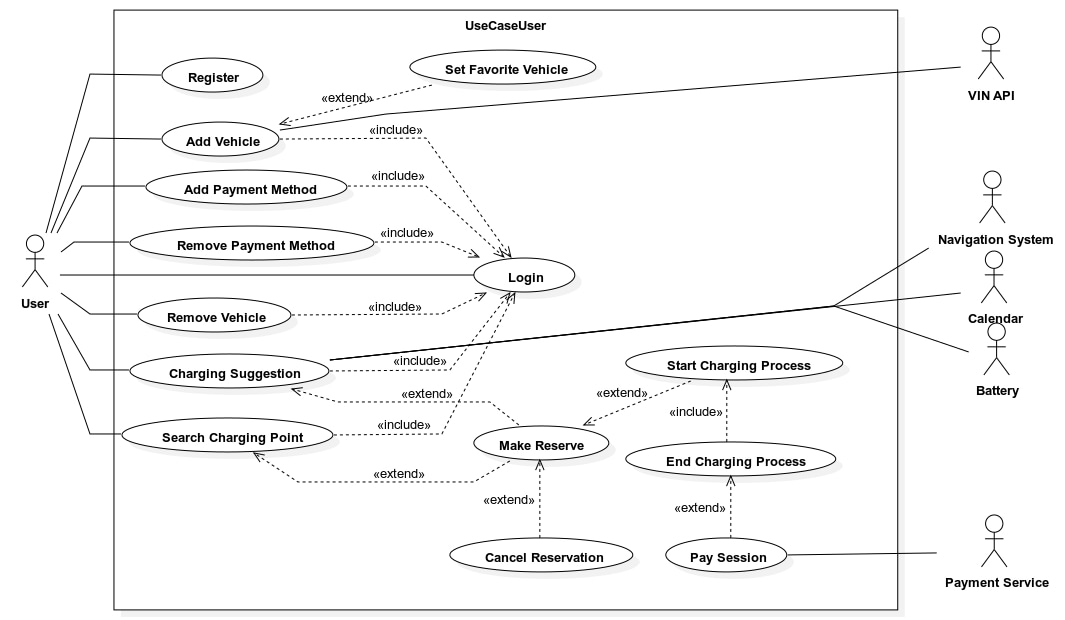
\includegraphics[width=1\textwidth]{Images/UseCases/UserUseCases.jpg}
    \caption{User Use Cases}
\end{figure}

% User Registration

\begin{table}[H]
    \begin{xltabular}{\textwidth}{| >{\columncolor{bluepoli!40}}l | X |}
    \hline
    \rowcolor{bluepoli!40}
    \textbf{ID} & \textbf{UC1}\T\B\\
    \hline
    \rowcolor{bluepoli!40}
    \textbf{Name} & \textbf{User Registration}\T\B\\
    \hline \hline
    \textbf{Actor} & User\T\B \\
    \hline
    \textbf{Entry Condition} & The user does not have an account and is on the login view\T\B\\
    \hline
    \textbf{Event Flow} & 
        \begin{enumerate}
        \item The user presses the “Register account” button;
        \item The page with the registration form shows up;
        \item The user compiles the required fields(email, password, confirm password, name, surname);
        \item The eMSP validates the data;
        \item The eMSP sends a confirmation email with a code;
        \item The user inserts the code of the email in the form;
        \item The eMSP creates the user;
        \item The eMSP displays a success message.
        \end{enumerate}\B\\
    \hline
    \textbf{Exit Conditions} & The user account is created\B\\
    \hline
    \textbf{Exceptions} & \begin{enumerate}
        \item The user does not enter all mandatory data;
        \item The user data aren’t valid;
        \item The user already exists;
        \item The user does not enter the correct confirmation code.
    \end{enumerate}
    \begin{itemize}
        \item In all cases the eMSP will notify the user.
    \end{itemize}\B\\
    \hline
    \end{xltabular}
\end{table}

\begin{figure}[H]
    \centering
    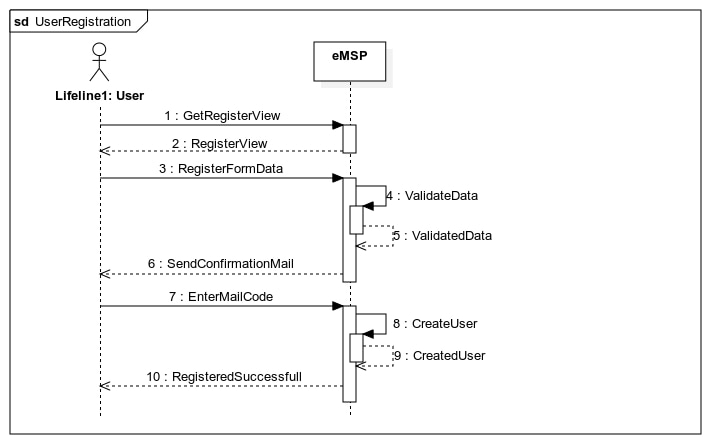
\includegraphics[width=1\textwidth]{Images/UseCases/UserRegistration.jpg}
    \caption{User Registration}
\end{figure}

% User Login

\newpage\begin{table}[H]
    \begin{xltabular}{\textwidth}{| >{\columncolor{bluepoli!40}}l | X |}
    \hline
    \rowcolor{bluepoli!40}
    \textbf{ID} & \textbf{UC2}\T\B\\
    \hline
    \rowcolor{bluepoli!40}
    \textbf{Name} & \textbf{User Login}\T\B\\
    \hline \hline
    \textbf{Actor} & User\T\B \\
    \hline
    \textbf{Entry Condition} & The user is registered but not logged in and is on the login view\T\B\\
    \hline
    \textbf{Event Flow} & 
        \begin{enumerate}
        \item The user inserts the combination of his email and password;
        \item The eMSP processes the information;
        \item The eMSP displays a success message.
        \end{enumerate}\B\\
    \hline
    \textbf{Exit Conditions} & The user is logged into the eMSP\B\\
    \hline
    \textbf{Exceptions} & \begin{enumerate}
        \item The user does not enter his credentials before submitting;
        \item The user enters invalid credentials.
        \end{enumerate}
        \begin{itemize}
            \item In all cases the eMSP will notify the user.
        \end{itemize}\B\\
    \hline
    \end{xltabular}
\end{table}

\begin{figure}[H]
    \centering
    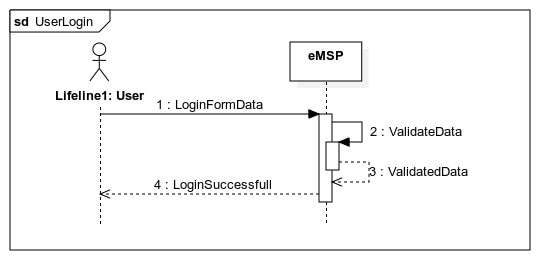
\includegraphics[width=1\textwidth]{Images/UseCases/UserLogin.jpg}
    \caption{User Login}
\end{figure}

% Add Vehicle

\begin{table}[H]
    \begin{xltabular}{\textwidth}{| >{\columncolor{bluepoli!40}}l | X |}
    \hline
    \rowcolor{bluepoli!40}
    \textbf{ID} & \textbf{UC3}\T\B\\
    \hline
    \rowcolor{bluepoli!40}
    \textbf{Name} & \textbf{Add Vehicle}\T\B\\
    \hline \hline
    \textbf{Actor} & User, VIN API\T\B \\
    \hline
    \textbf{Entry Condition} & The user is on the main menu of the application page\T\B\\
    \hline
    \textbf{Event Flow} & 
        \begin{enumerate}
        \item The user selects the overview of the vehicle;
        \item The eMSP retrieves a list of all vehicles provided by the user;
        \item The user selects the “add new vehicle” option;
        \item The eMSP displays a form in which the user can select the car to insert providing the VIN  code;
        \item The user inserts the VIN code of his car;
        \item The eMSP checks the VIN validity by sending a message to the VIN API;
        \item The VIN API sends a response to the eMSP;
        \item The eMSP shows a summary of the information regarding his car and asks for confirmation;
        \item The user chooses the confirm option;
        \item The eMSP displays a success message;
        \item The user set it as "favourite vehicle".
        \end{enumerate}\B\\
    \hline
    \textbf{Exit Conditions} & A new vehicle is inserted as favourite\B\\
    \hline
    \textbf{Exceptions} & 
        The VIN code provided is not correct.
        \begin{itemize}
            \item The eMSP asks the user to insert the correct code.
        \end{itemize}\B\\
    \hline
    \end{xltabular}
\end{table}

\begin{figure}[H]
    \centering
    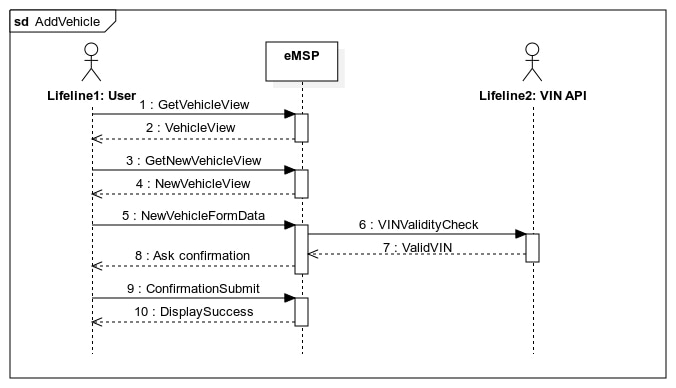
\includegraphics[width=1\textwidth]{Images/UseCases/AddVehicle.jpg}
    \caption{Add Vehicle}
\end{figure}

% Set Favourite Vehicle

\newpage\begin{table}[H]
    \begin{xltabular}{\textwidth}{| >{\columncolor{bluepoli!40}}l | X |}
    \hline
    \rowcolor{bluepoli!40}
    \textbf{ID} & \textbf{UC4}\T\B\\
    \hline
    \rowcolor{bluepoli!40}
    \textbf{Name} & \textbf{Set Favourite Vehicle}\T\B\\
    \hline \hline
    \textbf{Actor} & User\T\B \\
    \hline
    \textbf{Entry Condition} & The user is on the main menu of the application\T\B\\
    \hline
    \textbf{Event Flow} & 
        \begin{enumerate}
        \item The user selects the vehicle overview;
        \item The eMSP retrieves a list of all vehicles provided by the user;
        \item The user selects a vehicle;
        \item The eMSP displays a summary of all vehicle information;
        \item The user selects the “set as Favourite” option;
        \item The eMSP display a success message.
        \end{enumerate}\B\\
    \hline
    \textbf{Exit Conditions} & The vehicle is set as favourite from the eMSP\B\\
    \hline
    \textbf{Exceptions} & The vehicle doesn't exists\B\\
    \hline
    \end{xltabular}
\end{table}

\begin{figure}[H]
    \centering
    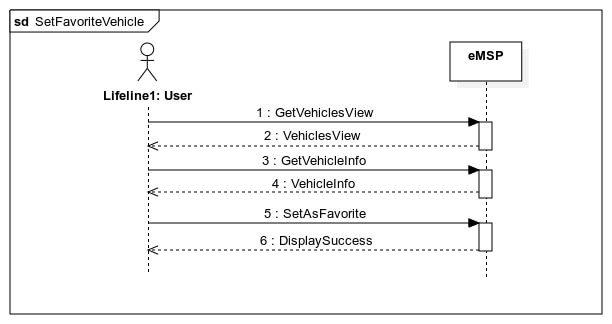
\includegraphics[width=1\textwidth]{Images/UseCases/SetFavouriteVehicle.jpg}
    \caption{Set Favourite Vehicle}
\end{figure}

% Remove Vehicle

\begin{table}[H]
    \begin{xltabular}{\textwidth}{| >{\columncolor{bluepoli!40}}l | X |}
    \hline
    \rowcolor{bluepoli!40}
    \textbf{ID} & \textbf{UC5}\T\B\\
    \hline
    \rowcolor{bluepoli!40}
    \textbf{Name} & \textbf{Remove Vehicle}\T\B\\
    \hline \hline
    \textbf{Actor} & User\T\B \\
    \hline
    \textbf{Entry Condition} & The user is on the main menu of the application\T\B\\
    \hline
    \textbf{Event Flow} & 
        \begin{enumerate}
        \item The user selects the vehicle overview;
        \item The eMSP retrieves a list of all vehicles provided by the user;
        \item The user selects a vehicle;
        \item The eMSP displays a summary of all vehicle information;
        \item The user selects the “remove vehicle” option;
        \item The eMSP asks for confirmation;
        \item The user confirms the action;
        \item The eMSP display a success message.
        \end{enumerate}\B\\
    \hline
    \textbf{Exit Conditions} & The vehicle is removed from the eMSP\B\\
    \hline
    \textbf{Exceptions} & The vehicle doesn't exists\B\\
    \hline
    \end{xltabular}
\end{table}

\begin{figure}[H]
    \centering
    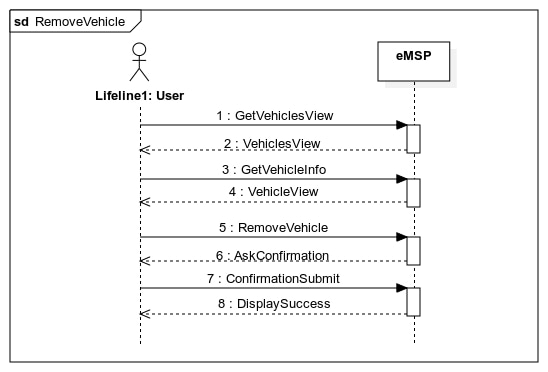
\includegraphics[width=0.8\textwidth]{Images/UseCases/RemoveVehicle.jpg}
    \caption{Remove Vehicle}
\end{figure}

% Add Payment Method

\newpage\begin{table}[H]
    \begin{xltabular}{\textwidth}{| >{\columncolor{bluepoli!40}}l | X |}
    \hline
    \rowcolor{bluepoli!40}
    \textbf{ID} & \textbf{UC6}\T\B\\
    \hline
    \rowcolor{bluepoli!40}
    \textbf{Name} & \textbf{Add Payment Method}\T\B\\
    \hline \hline
    \textbf{Actor} & User, Payment Service\T\B \\
    \hline
    \textbf{Entry Condition} & The user is logged in and in the payment methods page\T\B\\
    \hline
    \textbf{Event Flow} & 
        \begin{enumerate}
        \item The user clicks the “Add Payment Method” button;
        \item The eMSP shows the add payment method form;
        \item The user sends the payment information to the eMSP;
        \item The eMSP sends the information to the payment service for validation;
        \item The payment service responds with a valid message;
        \item The eMSP display a success message.
        \end{enumerate}\B\\
    \hline
    \textbf{Exit Conditions} & A new Payment Method is created\B\\
    \hline
    \textbf{Exceptions} & The payment method isn't valid. In this case, the eMSP will notify the user.\B\\
    \hline
    \end{xltabular}
\end{table}

\begin{figure}[H]
    \centering
    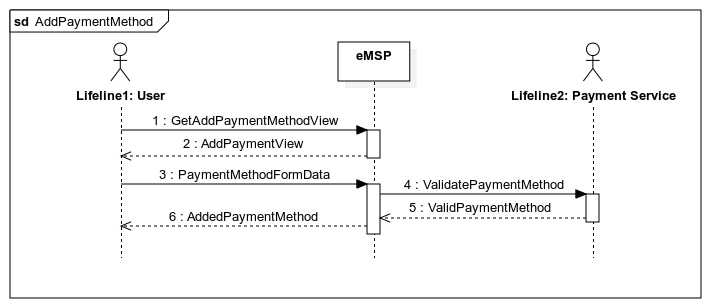
\includegraphics[width=1\textwidth]{Images/UseCases/AddPaymentMethod.jpg}
    \caption{Add Payment Method}
\end{figure}

% Remove Payment Method

\begin{table}[H]
    \begin{xltabular}{\textwidth}{| >{\columncolor{bluepoli!40}}l | X |}
    \hline
    \rowcolor{bluepoli!40}
    \textbf{ID} & \textbf{UC7}\T\B\\
    \hline
    \rowcolor{bluepoli!40}
    \textbf{Name} & \textbf{Remove Payment Method}\T\B\\
    \hline \hline
    \textbf{Actor} & User\T\B \\
    \hline
    \textbf{Entry Condition} & The user is logged in and in the payment methods page\T\B\\
    \hline
    \textbf{Event Flow} & 
        \begin{enumerate}
        \item The user clicks on the payment method that he wants to delete;
        \item The eMSP displays the payment method information;
        \item The user clicks on the “Delete” button;
        \item The system asks for confirmation;
        \item The eMSP display a success message.
        \end{enumerate}\B\\
    \hline
    \textbf{Exit Conditions} & The payment method is removed\B\\
    \hline
    \textbf{Exceptions} & The payment method doesn’t exist\B\\
    \hline
    \end{xltabular}
\end{table}

\begin{figure}[H]
    \centering
    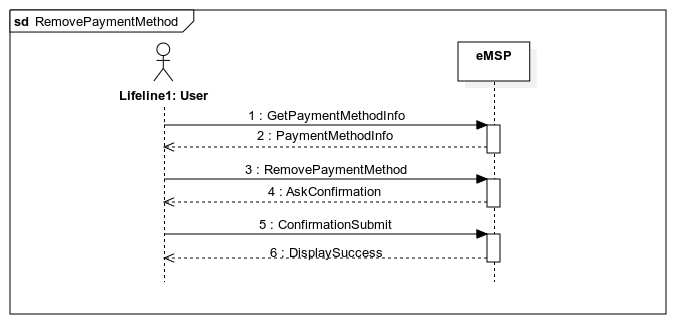
\includegraphics[width=1\textwidth]{Images/UseCases/RemovePaymentMethod.jpg}
    \caption{Remove Payment Method}
\end{figure}

% Make reservation

\begin{table}[H]
    \begin{xltabular}{\textwidth}{| >{\columncolor{bluepoli!40}}l | X |}
    \hline
    \rowcolor{bluepoli!40}
    \textbf{ID} & \textbf{UC8}\T\B\\
    \hline
    \rowcolor{bluepoli!40}
    \textbf{Name} & \textbf{Make Reservation}\T\B\\
    \hline \hline
    \textbf{Actor} & User, CP\T\B \\
    \hline
    \textbf{Entry Condition} & The user is logged in and is on the map page\T\B\\
    \hline
    \textbf{Event Flow} & 
        \begin{enumerate}
        \item The user requests CP info in an area by moving into the map view;
        \item The eMSP displays in the map portion, the CP distinguish by three cases:
        \begin{enumerate}
            \item At least a free socket is compatible with the favourite vehicle;
            \item All sockets compatible with the favourite vehicle are busy;
            \item All sockets are incompatible with the favourite vehicle.
        \end{enumerate}
        \item The user clicks on one of the visualized stations;
        \item The eMSP sends a CP’s info request to the CPMS;
        \item The CPMS sends the CP info to the eMSP;
        \item The eMSP displays the station information;
        \item The user selects a free socket;
        \item The eMSP displays socket information;
        \item The user clicks the reserve button;
        \item The eMSP checks that the user doesn’t have not paid sessions or active reservations;
        \item The eMSP sends the reserve request to the CPMS;
        \item The CPMS sends the reserve to the CP;
        \item The CP sends the response to the CPMS;
        \item The CPMS sends the response to the eMSP;
        \item The eMSP displays a success message.
        \end{enumerate}\B\\
    \hline
    \textbf{Exit Conditions} & The user reservation is created\B\\
    \hline
    \textbf{Exceptions} & \begin{enumerate}
        \item The user has an old not paid session;
        \item The user already has an active reservation;
        \item The selected socket is no more available.
    \end{enumerate}
    \begin{itemize}
        \item In all cases the eMSP will notify the user and prevent the reservation.
    \end{itemize}\B\\
    \hline
    \end{xltabular}
\end{table}

\begin{figure}[H]
    \centering
    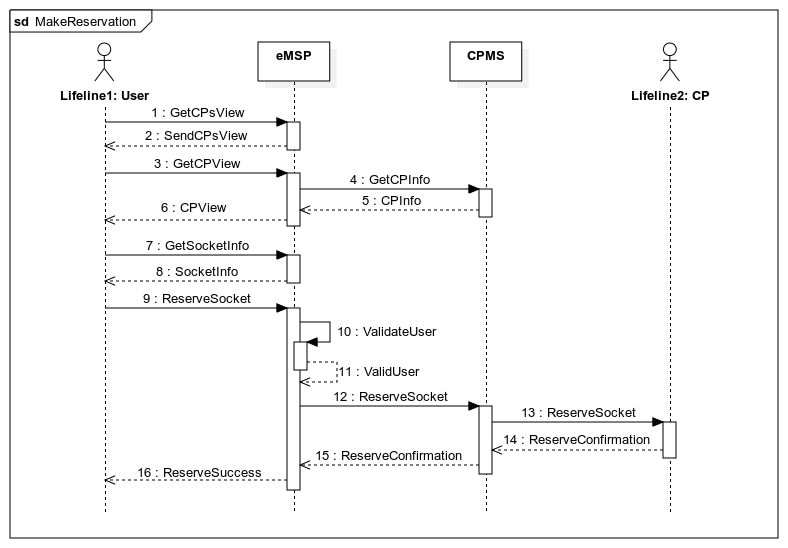
\includegraphics[width=1\textwidth]{Images/UseCases/MakeReservation.jpg}
    \caption{Make reservation}
\end{figure}

% Manage charging suggestions

\begin{table}[H]
    \begin{xltabular}{\textwidth}{| >{\columncolor{bluepoli!40}}l | X |}
    \hline
    \rowcolor{bluepoli!40}
    \textbf{ID} & \textbf{UC9}\T\B\\
    \hline
    \rowcolor{bluepoli!40}
    \textbf{Name} & \textbf{Manage Charging Suggestion}\T\B\\
    \hline \hline
    \textbf{Actor} & User, Navigation System, Calendar, Battery, CP\T\B \\
    \hline
    \textbf{Entry Condition} & The user favourite vehicle has a low battery\T\B\\
    \hline
    \textbf{Event Flow} & 
        \begin{enumerate}
        \item The eMSP retrieves the favourite vehicle’s  battery status through API;
        \item The eMSP retrieves the position from the GPS of the user;
        \item The eMSP retrieves the schedule of the user through the calendar;
        \item The eMSP retrieves the current navigation path, if present, of the user through its Navigation System;
        \item The eMSP computes the best set of CP to charge the Vehicle;
        \item The eMSP sends a notification to the User including the resume of the suggested stops;
        \item The User opens the application from the popup notification;
        \item The eMSP display the charging suggestion resume;
        \item The User accepts the charging suggestion;
        \item The eMSP checks that the user doesn’t have paid sessions;
        \item The eMSP sends the reserve request to the CPMS;
        \item The CPMS sends the reserve to the CP;
        \item The CP sends the response to the CPMS;
        \item The CPMS sends the response to the eMSP;
        \item The eMSP displays a success message.
        \end{enumerate}\B\\
    \hline
    \textbf{Exit Conditions} & The eMSP completes the reservation process\B\\
    \hline
    \textbf{Exceptions} & \begin{enumerate}
        \item The suggestion is declined;
        \item The reservation fails because the sockets are busy.
        \begin{itemize}
            \item In this case the eMSP calculates a new suggestion.
        \end{itemize}
        \end{enumerate}\B\\
    \hline
    \end{xltabular}
\end{table}

\begin{figure}[H]
    \centering
    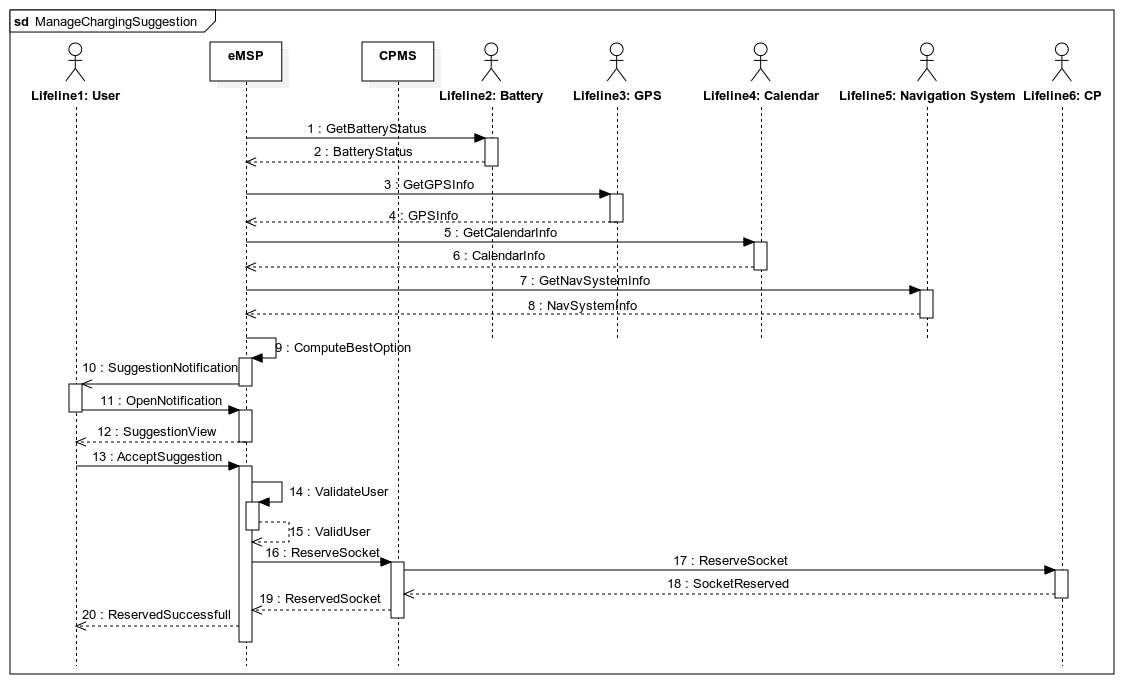
\includegraphics[width=1\textwidth]{Images/UseCases/ManageChargingSuggestion.jpg}
    \caption{Manage charging suggestions}
\end{figure}

% Cancel reservation

\begin{table}[H]
    \begin{xltabular}{\textwidth}{| >{\columncolor{bluepoli!40}}l | X |}
    \hline
    \rowcolor{bluepoli!40}
    \textbf{ID} & \textbf{UC10}\T\B\\
    \hline
    \rowcolor{bluepoli!40}
    \textbf{Name} & \textbf{Cancel Reservation}\T\B\\
    \hline \hline
    \textbf{Actor} & User, CP\T\B \\
    \hline
    \textbf{Entry Condition} & The user is logged in and is in the reservations tab\T\B\\
    \hline
    \textbf{Event Flow} & 
        \begin{enumerate}
        \item The user clicks on the current reservation;
        \item The user visualizes the current reservation information;
        \item The user clicks on the “Cancel Reservation” button;
        \item The eMSP sends the cancellation request to the CPMS;
        \item The CPMS sends the cancellation to the CP;
        \item The CP sends the response to the CPMS;
        \item The CPMS sends the response to the eMSP;
        \item The eMSP displays a success message.
        \end{enumerate}\B\\
    \hline
    \textbf{Exit Conditions} & The reservation status is updated to cancelled and the socket is available\B\\
    \hline
    \textbf{Exceptions} & 
    The reservation time is expired.
    \begin{itemize}
        \item In this case the system will notify the user.
    \end{itemize}\B\\
    \hline
    \end{xltabular}
\end{table}

\begin{figure}[H]
    \centering
    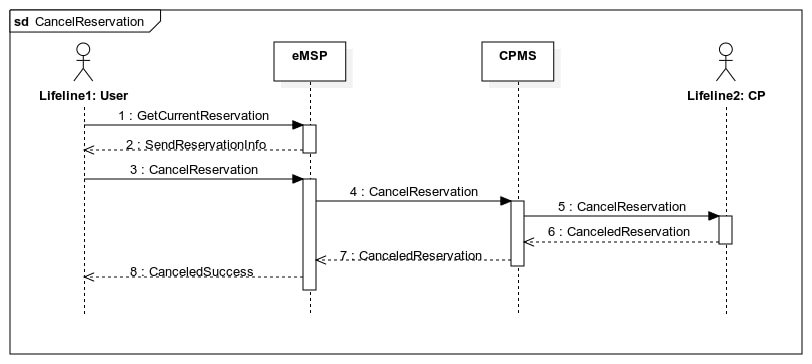
\includegraphics[width=1\textwidth]{Images/UseCases/CancelReservation.jpg}
    \caption{Cancel reservation}
\end{figure}

% Start Charging Process

\begin{table}[H]
    \begin{xltabular}{\textwidth}{| >{\columncolor{bluepoli!40}}l | X |}
    \hline
    \rowcolor{bluepoli!40}
    \textbf{ID} & \textbf{UC11}\T\B\\
    \hline
    \rowcolor{bluepoli!40}
    \textbf{Name} & \textbf{Start Charging Process}\T\B\\
    \hline \hline
    \textbf{Actor} & User, CP\T\B \\
    \hline
    \textbf{Entry Condition} & The user is logged in and in the current reservation tab\T\B\\
    \hline
    \textbf{Event Flow} & 
        \begin{enumerate}
        \item The user clicks the “Unlock” button;
        \item The eMSP sends the unlock socket request to the CPMS;
        \item The CPMS sends the unlock socket request to the CP;
        \item The CP unlocks the socket;
        \item The CP waits for the user to plug the socket;
        \item The CP recognizes a plugged socket;
        \item The CP sends the plugged socket message to CPMS;
        \item The CPMS sends the plugged socket message to eMSP;
        \item The eMSP shows the “Start charging” button;
        \item The user clicks the “Start charging” button;
        \item The eMSP sends the start transaction request to CPMS;
        \item The CPMS sends the start transaction request to CP;
        \item The CP locks the socket;
        \item The CP sends the response to the CPMS; 
        \item The CPMS sends the response to the eMSP;
        \item The eMSP displays a success message.
        \end{enumerate}\B\\
    \hline
    \textbf{Exit Conditions} & The charging process is started\B\\
    \hline
    \textbf{Exceptions} & 
    \begin{enumerate}
        \item The CP can’t unlock the socket;
        \item The CP can’t start the charging process;
        \item The user doesn't plug the socket correctly before pressing start charging.
    \end{enumerate}
    \begin{itemize}
        \item In all cases the eMSP will notify the user.
    \end{itemize}\B\\
    \hline
    \end{xltabular}
\end{table}

\begin{figure}[H]
    \centering
    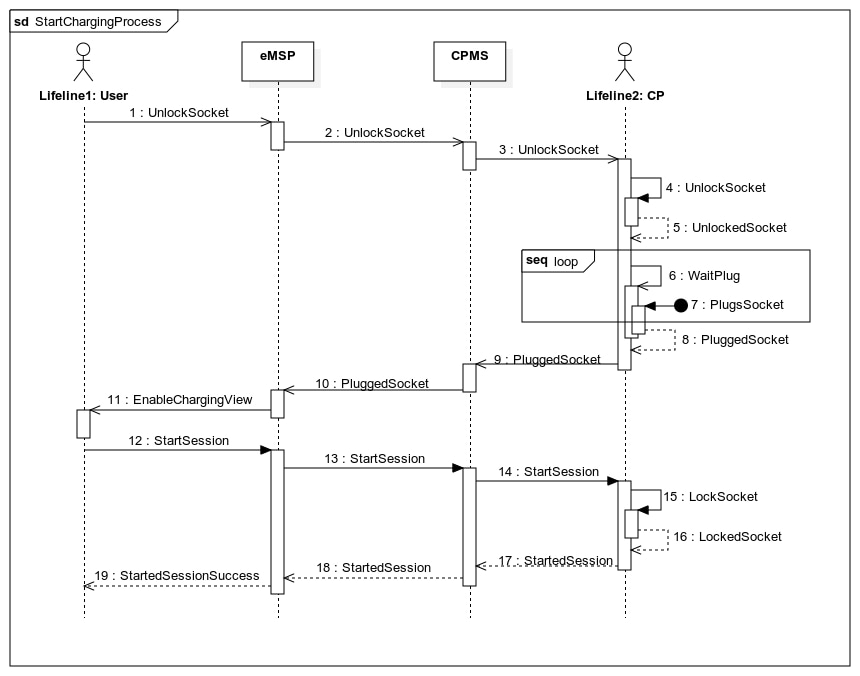
\includegraphics[width=1\textwidth]{Images/UseCases/StartChargingProcess.jpg}
    \caption{Start charging process}
\end{figure}

% End Charging Process

\begin{table}[H]
    \begin{xltabular}{\textwidth}{| >{\columncolor{bluepoli!40}}l | X |}
    \hline
    \rowcolor{bluepoli!40}
    \textbf{ID} & \textbf{UC12}\T\B\\
    \hline
    \rowcolor{bluepoli!40}
    \textbf{Name} & \textbf{End Charging Process}\T\B\\
    \hline \hline
    \textbf{Actor} & User, CP\T\B \\
    \hline
    \textbf{Entry Condition} & The user has an active charging session, is logged on and
        \begin{itemize}
            \item the battery of his car is full and he has received a notification for it, or
            \item had stopped the energy flow before the battery was full
        \end{itemize}\T\B\\
    \hline
    \textbf{Event Flow} & 
        \begin{enumerate}
        \item The user clicks on the current charging process button;
        \item The eMSP sends the charging session request to CPMS;
        \item The CPMS sends the charging session request to the CP;
        \item The CP sends the charging session to the CPMS;
        \item The CPMS sends the charging session to the eMSP;
        \item The eMSP displays the charging session to the user;
        \item The user clicks on the “end session” button;
        \item The eMSP sends the end charging session request to the CPMS;
        \item The CPMS sends the end charging session request to the CP;
        \item The CP unlocks the socket;
        \item The CP waits for the user to unplug the socket;
        \item The CP recognizes that the socket is unplugged;
        \item The CP sends the ended charging session response to the CPMS;
        \item The CPMS sends the ended charging session response to the eMSP;
        \item The eMSP displays a success message.
        \end{enumerate}\B\\
    \hline
    \textbf{Exit Conditions} & The charging process is ended\B\\
    \hline
    \textbf{Exceptions} & 
    \begin{enumerate}
        \item The charging process is already ended;
        \item The CP can’t stop the charging process.
    \end{enumerate}
    \begin{itemize}
        \item In all cases the system will notify the user.
    \end{itemize}\B\\
    \hline
    \end{xltabular}
\end{table}

\begin{figure}[H]
    \centering
    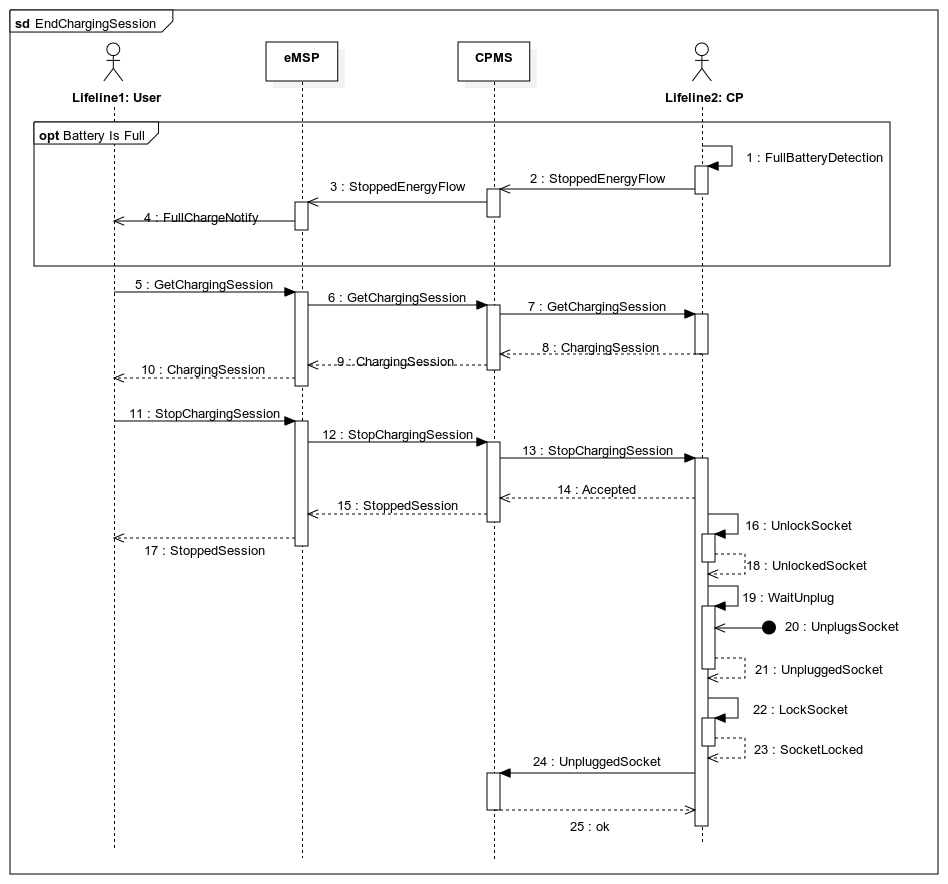
\includegraphics[width=1\textwidth]{Images/UseCases/EndChargingSession.jpg}
    \caption{End charging process}
\end{figure}

% Pay session

\begin{table}[H]
    \begin{xltabular}{\textwidth}{| >{\columncolor{bluepoli!40}}l | X |}
    \hline
    \rowcolor{bluepoli!40}
    \textbf{ID} & \textbf{UC13}\T\B\\
    \hline
    \rowcolor{bluepoli!40}
    \textbf{Name} & \textbf{Pay Session}\T\B\\
    \hline \hline
    \textbf{Actor} & User, Payment service\T\B \\
    \hline
    \textbf{Entry Condition} & 
    \begin{enumerate}
        \item The user is logged in and just ended the charging process;
        \item The user is logged in and clicks on pay not paid charging session.
    \end{enumerate}\T\B\\
    \hline
    \textbf{Event Flow} & 
        \begin{enumerate}
        \item The user selects one of its payment methods;
        \item The eMSP retrieves the user’s billing information;
        \item The eMSP retrieves the CPO’s billing information;
        \item The eMSP sends the information to the external payment service;
        \item The eMSP gets the response from the external payment service;
        \item The eMSP updates the payment status of the charging process.
        \end{enumerate}\B\\
    \hline
    \textbf{Exit Conditions} & The charging process is paid\B\\
    \hline
    \textbf{Exceptions} & 
    \begin{enumerate}
        \item The payment method is not valid;
        \item The external payment service returns an error.
    \end{enumerate}
    \begin{itemize}
        \item The eMSP adds the session to the not paid sessions.
    \end{itemize}\B\\
    \hline
    \end{xltabular}
\end{table}

\begin{figure}[H]
    \centering
    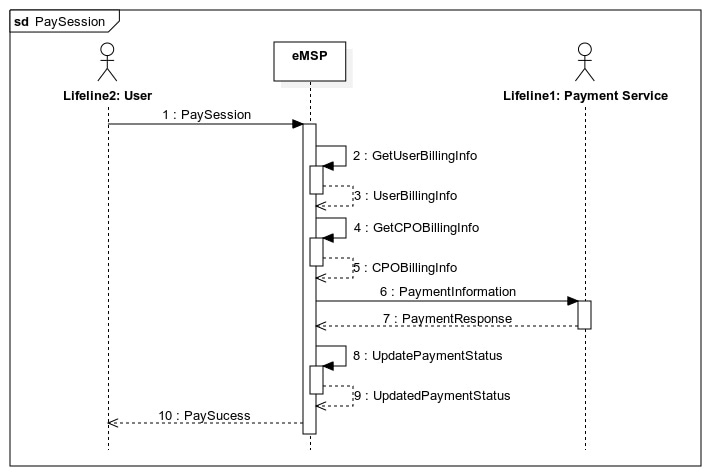
\includegraphics[width=1\textwidth]{Images/UseCases/PaySession.jpg}
    \caption{Pay Session}
\end{figure}

\subsection{CPO Use Cases}
\begin{figure}[H]
    \centering
    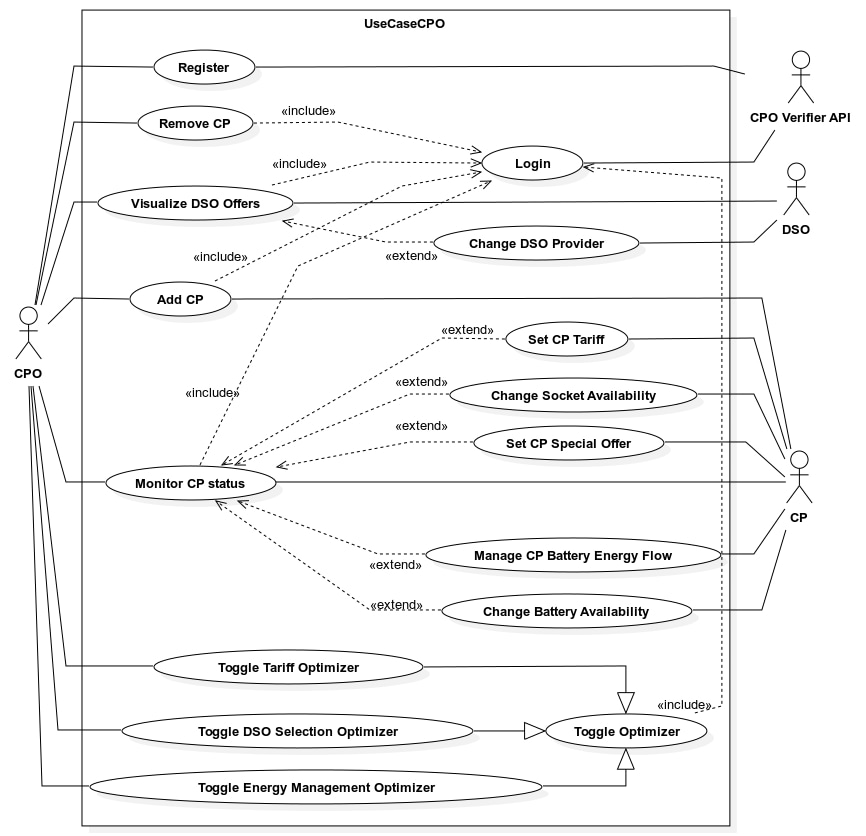
\includegraphics[width=1\textwidth]{Images/UseCases/CPOUseCases.jpg}
    \caption{CPO Use Cases}
\end{figure}

% CPO Registration

\begin{table}[H]
    \begin{xltabular}{\textwidth}{| >{\columncolor{bluepoli!40}}l | X |}
    \hline
    \rowcolor{bluepoli!40}
    \textbf{ID} & \textbf{UC14}\T\B\\
    \hline
    \rowcolor{bluepoli!40}
    \textbf{Name} & \textbf{CPO Registration}\T\B\\
    \hline \hline
    \textbf{Actor} & CPO, CPO Verifier API\T\B \\
    \hline
    \textbf{Entry Condition} & The CPO does not have an account and is on the login view\T\B\\
    \hline
    \textbf{Event Flow} & 
        \begin{enumerate}
        \item The CPO presses the “Register account” button;
        \item The page with the registration form shows up;
        \item The user compiles the required fields(CPOCode, Password, Confirm password);
        \item The CPMS sends the CPOCode to an external verifier API;
        \item The CPO Verifier API sends the confirmation to the CPMS;
        \item The CPMS displays a success message.
        \end{enumerate}\B\\
    \hline
    \textbf{Exit Conditions} & The CPO account is created\B\\
    \hline
    \textbf{Exceptions} & \begin{enumerate}
        \item The CPO does not enter all mandatory data;
        \item The CPO data aren’t valid;
        \item The CPO already exists.
        \end{enumerate}
        \begin{itemize}
            \item In all cases the CPMS will notify the CPO.
        \end{itemize}\B\\
    \hline
    \end{xltabular}
\end{table}

\begin{figure}[H]
    \centering
    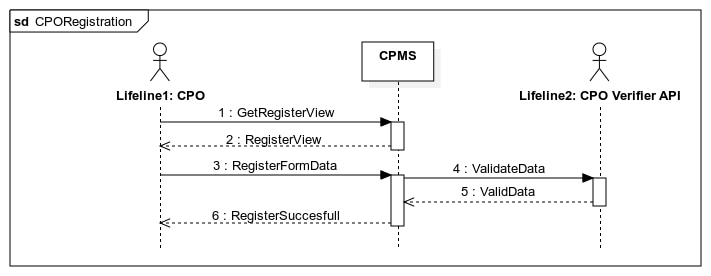
\includegraphics[width=1\textwidth]{Images/UseCases/CPORegistration.jpg}
    \caption{CPO Registration}
\end{figure}

% CPO Login

\newpage\begin{table}[H]
    \begin{xltabular}{\textwidth}{| >{\columncolor{bluepoli!40}}l | X |}
    \hline
    \rowcolor{bluepoli!40}
    \textbf{ID} & \textbf{UC15}\T\B\\
    \hline
    \rowcolor{bluepoli!40}
    \textbf{Name} & \textbf{CPO Login}\T\B\\
    \hline \hline
    \textbf{Actor} & CPO, CPO Verifier API\T\B \\
    \hline
    \textbf{Entry Condition} & The CPO is registered but not logged in and is on the login view\T\B\\
    \hline
    \textbf{Event Flow} & 
        \begin{enumerate}
        \item The user inserts the combination of his CPOCode and password;
        \item The CPMS sends the data to the CPO Verifier API for verification;
        \item The CPO Verifier API sends the confirmation to the CPMS;
        \item The CPMS displays a success message.
        \end{enumerate}\B\\
    \hline
    \textbf{Exit Conditions} & The CPO is logged into the CPMS\B\\
    \hline
    \textbf{Exceptions} & \begin{enumerate}
        \item The CPO does not enter his credentials before submitting;
        \item The CPO enters invalid credentials.
        \end{enumerate}
        \begin{itemize}
            \item In all cases the CPMS will notify the user.
        \end{itemize}\B\\
    \hline
    \end{xltabular}
\end{table}

\begin{figure}[H]
    \centering
    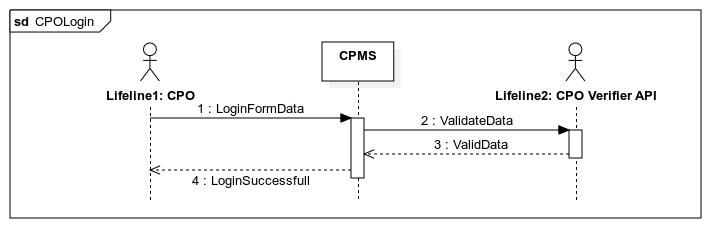
\includegraphics[width=1\textwidth]{Images/UseCases/CPOLogin.jpg}
    \caption{CPO Login}
\end{figure}

% ADD CP

\begin{table}[H]
    \begin{xltabular}{\textwidth}{| >{\columncolor{bluepoli!40}}l | X |}
    \hline
    \rowcolor{bluepoli!40}
    \textbf{ID} & \textbf{UC16}\T\B\\
    \hline
    \rowcolor{bluepoli!40}
    \textbf{Name} & \textbf{Add CP}\T\B\\
    \hline \hline
    \textbf{Actor} & CPO, CP\T\B \\
    \hline
    \textbf{Entry Condition} & The CPO is logged on the CPMS and is on the home page\T\B\\
    \hline
    \textbf{Event Flow} & 
        \begin{enumerate}
        \item The CPO presses the “Add charging point” button;
        \item The CPMS displays a form to the CPO;
        \item The CPO insert the location of the CP, a list of sockets together with their type, and the price of energy that will be applied in that CP;
        \item The CPO inserts some information about how the CPMS will be able to connect to the new CP;
        \item The CPMS establishes a connection to the new charging point;
        \item The new charging point accepts the connection and acknowledges the CPMS;
        \item The CPMS notify to all the eMSP of the presence of the new charging point.
        \end{enumerate}\B\\
    \hline
    \textbf{Exit Conditions} & The CPMS shows the home page to the CPO, where the new charging point is present\B\\
    \hline
    \textbf{Exceptions} & If the CPMS is not able to connect to the new charging point, it warns the CPO that can modify the connection parameters or remove the charging point\B\\
    \hline
    \end{xltabular}
\end{table}

\begin{figure}[H]
    \centering
    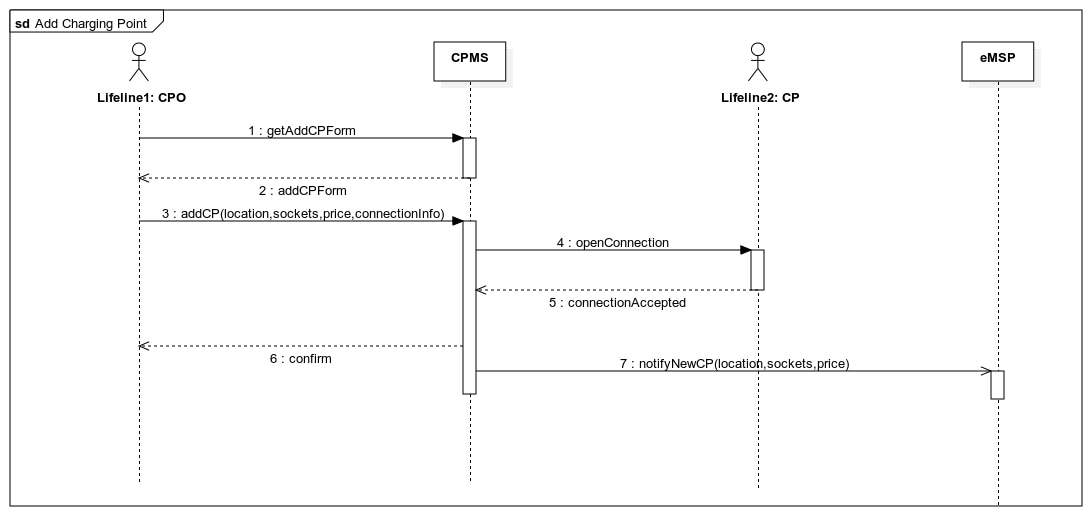
\includegraphics[width=1\textwidth]{Images/UseCases/AddCP.jpg}
    \caption{Add CP}
\end{figure}

% MANAGE CP'S BATTERY CONNECTION

\begin{table}[H]
    \begin{xltabular}{\textwidth}{| >{\columncolor{bluepoli!40}}l | X |}
    \hline
    \rowcolor{bluepoli!40}
    \textbf{ID} & \textbf{UC17}\T\B\\
    \hline
    \rowcolor{bluepoli!40}
    \textbf{Name} & \textbf{Manage CP’s battery  energy flow}\T\B\\
    \hline \hline
    \textbf{Actor} & CPO, CP\T\B \\
    \hline
    \textbf{Entry Condition} & The CPO is logged on the CPMS, in the Manual Mode and is viewing the internal status of the charging point.\T\B\\
    \hline
    \textbf{Event Flow} & 
        \begin{enumerate}
        \item The CPO presses the “Manage Energy Source” button;
        \item CPMS shows a page that contains details about the battery status and about the current energy sources;
        \item The CPO presses the “Include battery” button;
        \item The CPMS shows a form to the CPO;
        \item The CPO inserts the percentage of energy that the charging point will take from the battery for the charging sessions and the minimum and maximum battery levels;
        \item The CPMS notifies the charging point about the change of strategy for the energy flow;
        \item The charging point confirms the update;
        \item The CPMS shows a success message to the CPO.
        \end{enumerate}\B\\
    \hline
    \textbf{Exit Conditions} & The battery is added to the current energy sources.\B\\
    \hline
    \textbf{Exceptions} & If the minimum battery level is higher than the maximum battery level the CPMS will notify the CPO, which will have to change the parameters.\B\\
    \hline
    \end{xltabular}
\end{table}

\begin{figure}[H]
    \centering
    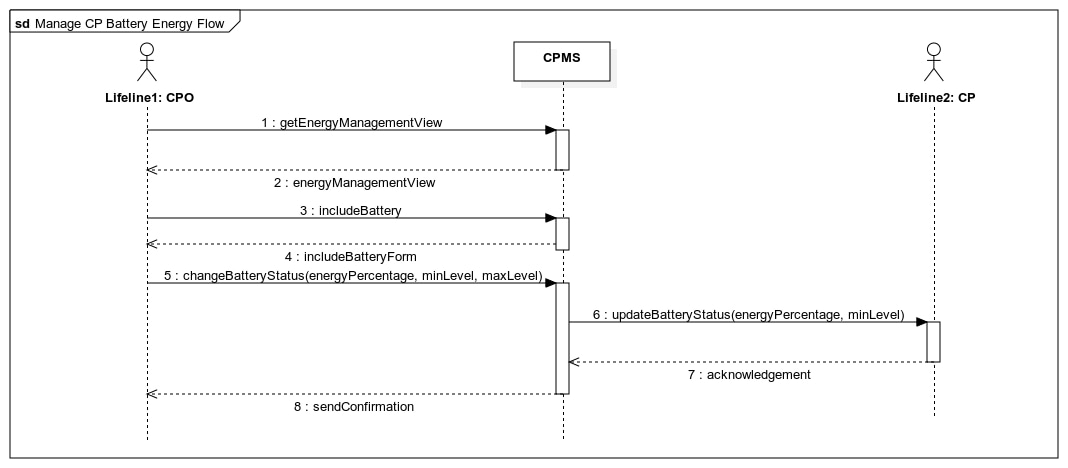
\includegraphics[width=1\textwidth]{Images/UseCases/ManageCPsBatteryEnergyFlow.jpg}
    \caption{Manage CP’s battery  energy flow}
\end{figure}

% Change the socket’s  availability

\begin{table}[H]
    \begin{xltabular}{\textwidth}{| >{\columncolor{bluepoli!40}}l | X |}
    \hline
    \rowcolor{bluepoli!40}
    \textbf{ID} & \textbf{UC18}\T\B\\
    \hline
    \rowcolor{bluepoli!40}
    \textbf{Name} & \textbf{Change the socket’s  availability}\T\B\\
    \hline \hline
    \textbf{Actor} & CPO, CP\T\B \\
    \hline
    \textbf{Entry Condition} & The CPO is logged on the CPMS and is on the home page\T\B\\
    \hline
    \textbf{Event Flow} & 
        \begin{enumerate}
        \item The CPO press the “CP View” button;
        \item The CPMS shows a page containing CP information;
        \item The CPO press the “Manage Sockets” button relative to a certain CP;
        \item The CPMS shows a page containing all the sockets of a certain CP, including the type of sockets, the availability of the socket, how much energy the sockets are currently providing to the connected vehicles, and the estimated remaining time to complete the charging session;
        \item The CPO clicks the “Change availability” button near a socket;
        \item The CPMS shows a form where the CPO has to insert the starting date and time on which the socket will change the available;
        \item The CPO inserts the date and the new availability;
        \item The CPMS waits until the inserted time is reached;
        \item The CPMS notifies the change of availability of a socket to the charging point;
        \item The charging point confirms the update;
        \item The CPMS sends a notification to the CPO to confirm the update;
        \item The CPMS notifies all the connected eMSP about the update.
        \end{enumerate}\B\\
    \hline
    \textbf{Exit Conditions} & The CPMS returns to the page that shows the status of the sockets of the charging point\B\\
    \hline
    \textbf{Exceptions} & If there is a charging session that will terminate after the timestamp inserted by the CPO, the CPMS will send an error to the CPO\B\\
    \hline
    \end{xltabular}
\end{table}

\begin{figure}[H]
    \centering
    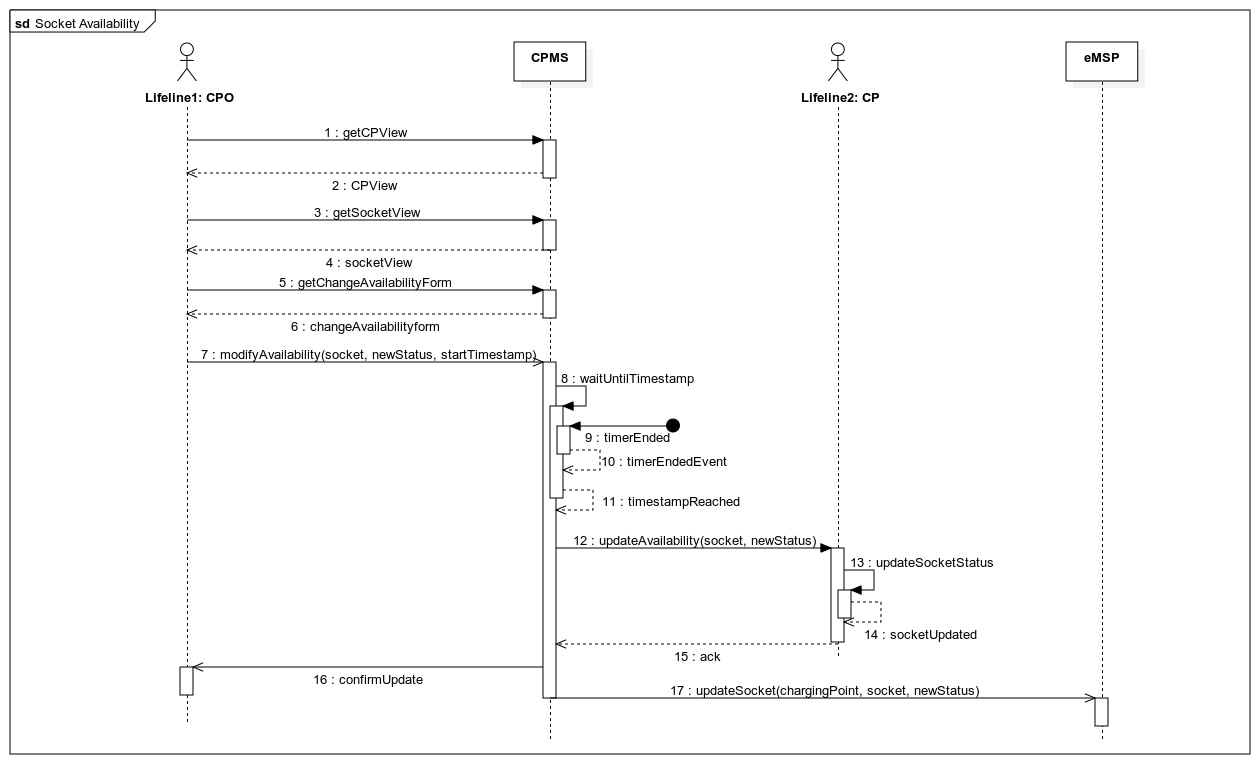
\includegraphics[width=1\textwidth]{Images/UseCases/ChangeSocketAvailability.jpg}
    \caption{Change the socket’s  availability}
\end{figure}

% Set charging point Tariff

\begin{table}[H]
    \begin{xltabular}{\textwidth}{| >{\columncolor{bluepoli!40}}l | X |}
    \hline
    \rowcolor{bluepoli!40}
    \textbf{ID} & \textbf{UC19}\T\B\\
    \hline
    \rowcolor{bluepoli!40}
    \textbf{Name} & \textbf{Set charging point Tariff}\T\B\\
    \hline \hline
    \textbf{Actor} & CPO\T\B \\
    \hline
    \textbf{Entry Condition} & The CPO is logged on the CPMS and is on the home page\T\B\\
    \hline
    \textbf{Event Flow} & 
        \begin{enumerate}
        \item The CPO press the “CP View” button;
        \item The CPMS shows a page containing CP information;
        \item The CPO presses the “Price Update” button;
        \item The CPMS shows a form to the CPO;
        \item The CPO inserts the new price of the charging station and submits the changes;
        \item The CPMS shows a success message;
        \item The CPMS notifies all the connected eMSP about the change in the price.
        \end{enumerate}\B\\
    \hline
    \textbf{Exit Conditions} & The price of the charging point is changed\B\\
    \hline
    \textbf{Exceptions} & If the price that the CPO insert is lower than the current price of energy that the CPO is paying to the DSO, the CPMS warns the CPO before applying the change\B\\
    \hline
    \end{xltabular}
\end{table}

\begin{figure}[H]
    \centering
    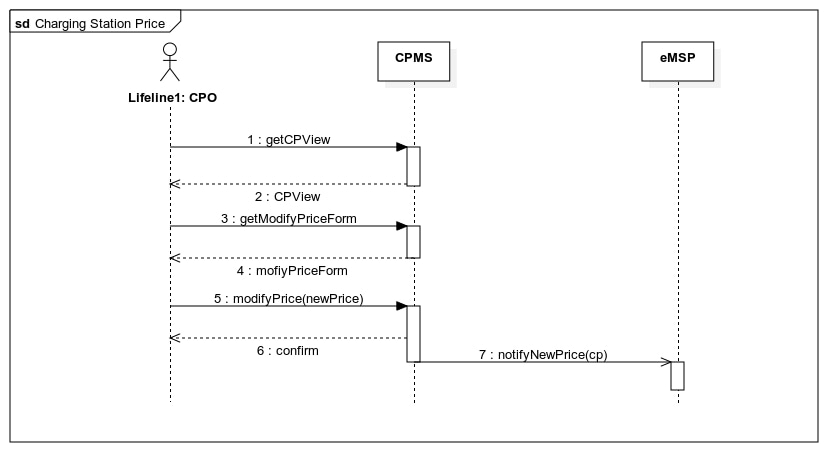
\includegraphics[width=0.9\textwidth]{Images/UseCases/SetChargingPointTariff.jpg}
    \caption{Set charging point Tariff}
\end{figure}

% Set charging point Special Offer

\begin{table}[H]
    \begin{xltabular}{\textwidth}{| >{\columncolor{bluepoli!40}}l | X |}
    \hline
    \rowcolor{bluepoli!40}
    \textbf{ID} & \textbf{UC20}\T\B\\
    \hline
    \rowcolor{bluepoli!40}
    \textbf{Name} & \textbf{Set charging point Special Offer}\T\B\\
    \hline \hline
    \textbf{Actor} & CPO\T\B \\
    \hline
    \textbf{Entry Condition} & The CPO is logged on the CPMS and is viewing the home page\T\B\\
    \hline
    \textbf{Event Flow} & 
        \begin{enumerate}
        \item The CPO press the “CP View” button;
        \item The CPMS shows a page containing CP information;
        \item The CPO presses the “Add special offer” button;
        \item The CPMS shows a form to the CPO;
        \item The CPO inserts the new special offer for the charging station, which includes the price and the period on which the offer will be valid;
        \item The CPMS shows a success message;
        \item The CPMS notifies all the connected eMSP about the change in the price.
        \end{enumerate}\B\\
    \hline
    \textbf{Exit Conditions} & A new special offer is created\B\\
    \hline
    \textbf{Exceptions} & If the price that the CPO insert is lower than the current price of energy that the CPO is paying to the DSO, the CPMS warns the CPO before applying the change\B\\
    \hline
    \end{xltabular}
\end{table}

\begin{figure}[H]
    \centering
    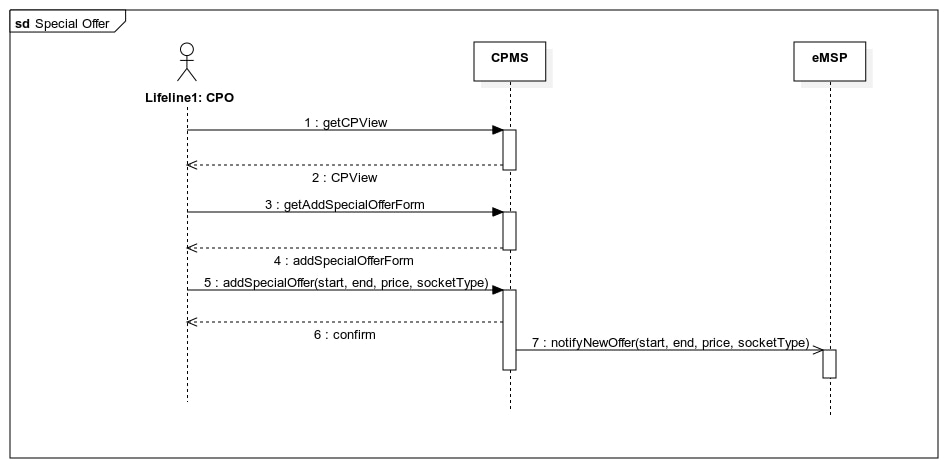
\includegraphics[width=0.9\textwidth]{Images/UseCases/SetChargingPointSpecialOffer.jpg}
    \caption{Set charging point Special Offer}
\end{figure}

% Remove CP

\newpage\begin{table}[H]
    \begin{xltabular}{\textwidth}{| >{\columncolor{bluepoli!40}}l | X |}
    \hline
    \rowcolor{bluepoli!40}
    \textbf{ID} & \textbf{UC21}\T\B\\
    \hline
    \rowcolor{bluepoli!40}
    \textbf{Name} & \textbf{Remove CP}\T\B\\
    \hline \hline
    \textbf{Actor} & CPO\T\B \\
    \hline
    \textbf{Entry Condition} & The CPO is logged in to the CPMS and is viewing the home page\T\B\\
    \hline
    \textbf{Event Flow} & 
        \begin{enumerate}
        \item The CPO presses the “Remove CP” button near a specific charging point;
        \item The CPMS shows a confirmation popup to the CPO;
        \item The CPO confirms the operation;
        \item The CPMS closes the connection with the charging point;
        \item The CPMS asynchronously notifies all the connected eMSP that the removed CP is no longer available.
        \end{enumerate}\B\\
    \hline
    \textbf{Exit Conditions} & The charging point is removed and the CPMS shows the home page to the CPO\B\\
    \hline
    \textbf{Exceptions} & If there are vehicles connected (or registered for a charging session that is not yet started) to some sockets of the charging point, the CPMS prevents the CPO from removing the charging point\B\\
    \hline
    \end{xltabular}
\end{table}

\begin{figure}[H]
    \centering
    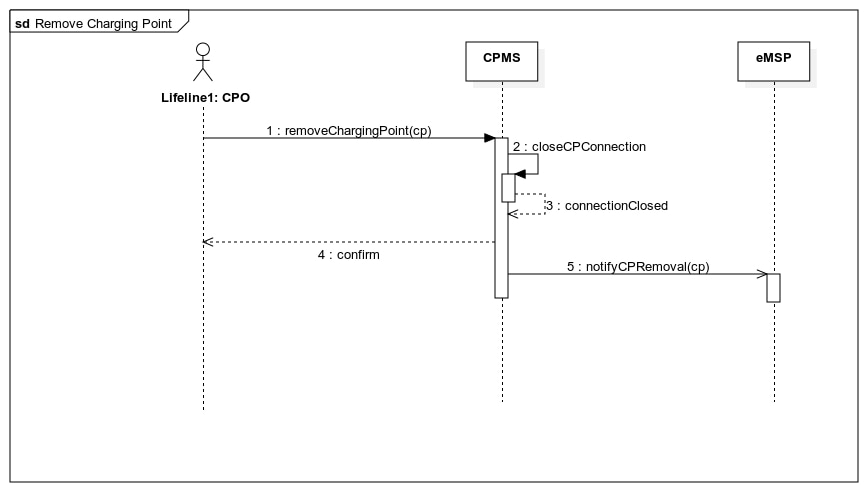
\includegraphics[width=0.9\textwidth]{Images/UseCases/RemoveCP.jpg}
    \caption{Remove CP}
\end{figure}

% Change DSO provider

\begin{table}[H]
    \begin{xltabular}{\textwidth}{| >{\columncolor{bluepoli!40}}l | X |}
    \hline
    \rowcolor{bluepoli!40}
    \textbf{ID} & \textbf{UC22}\T\B\\
    \hline
    \rowcolor{bluepoli!40}
    \textbf{Name} & \textbf{Change DSO provider}\T\B\\
    \hline \hline
    \textbf{Actor} & CPO, CP\T\B \\
    \hline
    \textbf{Entry Condition} & The CPO is logged in to the application and on and is on the main page view\T\B\\
    \hline
    \textbf{Event Flow} & 
        \begin{enumerate}
        \item The CPO selects a particular CP;
        \item The CPMS displays general CP information;
        \item The CPO press the “Manage Energy Source” button;
        \item The CPMS displays all information in detail including energy source and battery information;
        \item The CPO selects “DSOs’ offers”;
        \item The CPMS displays all available offers for that CP;
        \item The CPO select the “Offer detail” option to know about the detail related to an offer;
        \item The CPMS displays a page that includes all offers info and asks for a confirmation to change DSO provider;
        \item The CPO reads the resume and confirms the option selected;
        \item The CPMS sends a “change energy source” request to the CP;
        \item The CP changes the energy source and confirms the changes to the CPMS;
        \item The CPMS displays a confirmation message to the CPO.
        \end{enumerate}\B\\
    \hline
    \textbf{Exit Conditions} & The CPMS displays a success message to the CPO\B\\
    \hline
    \textbf{Exceptions} & \begin{enumerate}
        \item The CP is unable to change the energy source;
        \begin{itemize}
            \item An error message is displayed and the procedure is aborted.
        \end{itemize}
        \item The selected Energy offer is not able to provide the energy required to fulfill the CP’s charging profile.
        \begin{itemize}
            \item The CPMS displays a warning to the CP, asking for a change or confirmation.
        \end{itemize}
        \end{enumerate}\B\\
    \hline
    \end{xltabular}
\end{table}

\begin{figure}[H]
    \centering
    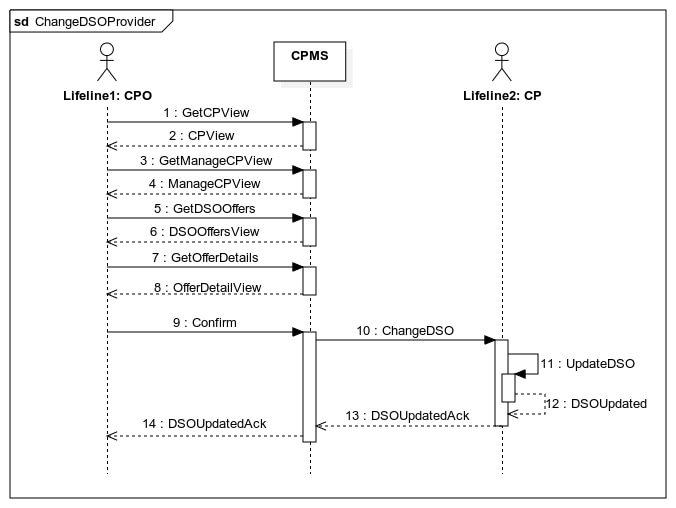
\includegraphics[width=1\textwidth]{Images/UseCases/ChangeDSOProvider.jpg}
    \caption{Change DSO provider}
\end{figure}

% Change Battery Av.

\begin{table}[H]
    \begin{xltabular}{\textwidth}{| >{\columncolor{bluepoli!40}}l | X |}
    \hline
    \rowcolor{bluepoli!40}
    \textbf{ID} & \textbf{UC23}\T\B\\
    \hline
    \rowcolor{bluepoli!40}
    \textbf{Name} & \textbf{Change Battery Availability}\T\B\\
    \hline \hline
    \textbf{Actor} & CPO, CP\T\B \\
    \hline
    \textbf{Entry Condition} & The CPO is logged in to the application and on and is on the main page view\T\B\\
    \hline
    \textbf{Event Flow} & 
        \begin{enumerate}
        \item The CPO selects a particular CP;
        \item The CPMS displays general CP information;
        \item The CPO press the “Manage Energy Source” button;
        \item The CPMS displays all information in detail including energy source and battery information;
        \item The CPO switch presses the button “Exclude Battery” to make the battery not available;
        \item The CPMS displays a message that asks the CPO to confirm the action;
        \item The CP confirms;
        \item The CPMS sends a “exclude battery request” to the CP;
        \item The CP confirms the battery update and the system excludes the battery from the system;
        \item The CPMS displays a success message.
        \end{enumerate}\B\\
    \hline
    \textbf{Exit Conditions} & The battery is excluded from the CP energy management system\B\\
    \hline
    \textbf{Exceptions} & \begin{enumerate}
        \item There is no DSO offer for the selected CP;
        \item The CP can’t exclude battery.
        \end{enumerate}\B\\
    \hline
    \end{xltabular}
\end{table}

\begin{figure}[H]
    \centering
    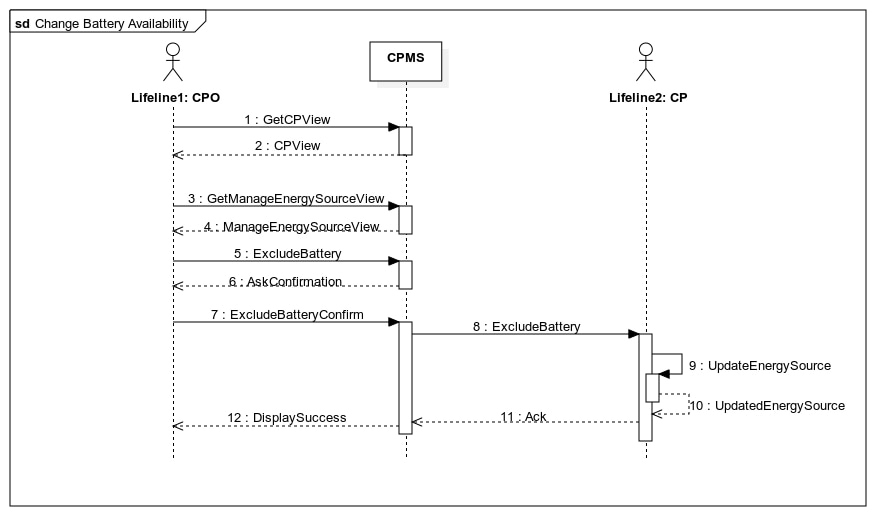
\includegraphics[width=1\textwidth]{Images/UseCases/Change Battery Availability.jpg}
    \caption{Change Battery Availability}
\end{figure}

% Toggle Tariff Optimizer

\newpage\begin{table}[H]
    \begin{xltabular}{\textwidth}{| >{\columncolor{bluepoli!40}}l | X |}
    \hline
    \rowcolor{bluepoli!40}
    \textbf{ID} & \textbf{UC24}\T\B\\
    \hline
    \rowcolor{bluepoli!40}
    \textbf{Name} & \textbf{Toggle Tariff Optimizer}\T\B\\
    \hline \hline
    \textbf{Actor} & CPO\T\B \\
    \hline
    \textbf{Entry Condition} & The CPO is logged in to the application and on and is on the main page view\T\B\\
    \hline
    \textbf{Event Flow} & 
        \begin{enumerate}
        \item The CPO selects a particular CP;
        \item The CPMS displays general CP information;
        \item The CPO press the “Optimizer” button;
        \item The CPMS displays all the Optimizer settings;
        \item The CPO compiles a form in order to select the optimizer settings for tariffs;
        \item The CPMS displays a success message.
        \end{enumerate}\B\\
    \hline
    \textbf{Exit Conditions} & The optimizer switch its state to on if is off or off if is on \B\\
    \hline
    \textbf{Exceptions} & The CP doesn't exists.\B\\
    \hline
    \end{xltabular}
\end{table}

\begin{figure}[H]
    \centering
    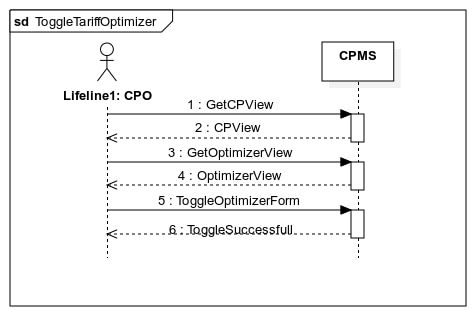
\includegraphics[width=0.7\textwidth]{Images/UseCases/ToggleTariffOptimizer.jpg}
    \caption{Toggle Tariff Optimizer}
\end{figure}

% Toggle DSO Selection Optimizer

\begin{table}[H]
    \begin{xltabular}{\textwidth}{| >{\columncolor{bluepoli!40}}l | X |}
    \hline
    \rowcolor{bluepoli!40}
    \textbf{ID} & \textbf{UC25}\T\B\\
    \hline
    \rowcolor{bluepoli!40}
    \textbf{Name} & \textbf{Toggle DSO Selection Optimizer}\T\B\\
    \hline \hline
    \textbf{Actor} & CPO\T\B \\
    \hline
    \textbf{Entry Condition} & The CPO is logged in to the application and on and is on the main page view\T\B\\
    \hline
    \textbf{Event Flow} & 
        \begin{enumerate}
        \item The CPO selects a particular CP;
        \item The CPMS displays general CP information;
        \item The CPO press the “Optimizer” button;
        \item The CPMS displays all the Optimizer settings;
        \item The CPO compiles a form in order to select the optimizer settings for DSO selection;
        \item The CPMS displays a success message.
        \end{enumerate}\B\\
    \hline
    \textbf{Exit Conditions} & The optimizer switch its state to on if is off or off if is on\B\\
    \hline
    \textbf{Exceptions} & 
        The CP doesn't exists.\B\\
    \hline
    \end{xltabular}
\end{table}

\begin{figure}[H]
    \centering
    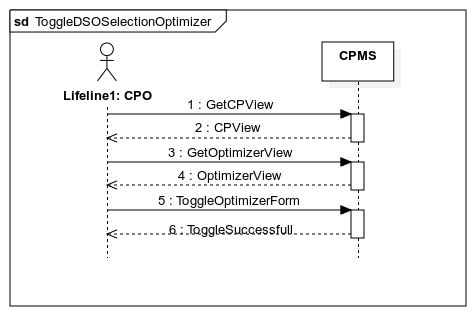
\includegraphics[width=0.7\textwidth]{Images/UseCases/ToggleDSOSelectionOptimizer.jpg}
    \caption{Toggle DSO Selection Optimizer}
\end{figure}

% Toggle Energy Management Optimizer

\begin{table}[H]
    \begin{xltabular}{\textwidth}{| >{\columncolor{bluepoli!40}}l | X |}
    \hline
    \rowcolor{bluepoli!40}
    \textbf{ID} & \textbf{UC26}\T\B\\
    \hline
    \rowcolor{bluepoli!40}
    \textbf{Name} & \textbf{Toggle Energy Management Optimizer}\T\B\\
    \hline \hline
    \textbf{Actor} & CPO\T\B \\
    \hline
    \textbf{Entry Condition} & The CPO is logged in to the application and on and is on the main page view\T\B\\
    \hline
    \textbf{Event Flow} & 
        \begin{enumerate}
        \item The CPO selects a particular CP;
        \item The CPMS displays general CP information;
        \item The CPO press the “Optimizer” button;
        \item The CPMS displays all the Optimizer settings;
        \item The CPO compiles a form in order to select the optimizer settings for energy management;
        \item The CPMS displays a success message.
        \end{enumerate}\B\\
    \hline
    \textbf{Exit Conditions} & The optimizer switch its state to on if is off or off if is on \B\\
    \hline
    \textbf{Exceptions} & 
        The CP doesn't exists.\B\\
    \hline
    \end{xltabular}
\end{table}

\begin{figure}[H]
    \centering
    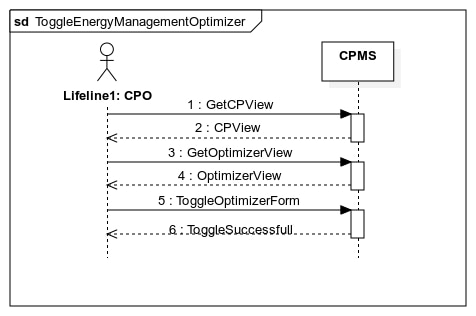
\includegraphics[width=0.7\textwidth]{Images/UseCases/ToggleEnergyManagementOptimizer.jpg}
    \caption{Toggle Energy Management Optimizer}
\end{figure}

\newpage\subsection{Requirements}

    \subsubsection{eMSP Requirements}

 \begin{xltabular}{\textwidth}{| >{\columncolor{bluepoli!40}}l | X |}
\hline
R1 &
    The eMSP shall allow unregistered users to register via e-mail and password. \B\\
\hline
 
R2  &
   The eMSP shall send a confirmation mail when a new user tries to register to it containing a code to confirm the account.\B\\
\hline

R3  &
    The eMSP shall allow the user to log in to the application using e-mail and password.\B\\
\hline

R4  &
    The eMSP shall allow a user to register a new vehicle using the VIN code.\B\\
\hline

R5  &
    The eMSP shall verify the validity of a VIN code inserted by a user.\B\\
\hline

R6  &
    The eMSP shall allow the selection of a vehicle as the favourite of a user.\B\\
\hline

R7  &
    The eMSP shall allow a user to remove a vehicle from the system and the relative data.\B\\
\hline

R8  &
   The eMSP shall allow the User to add a payment method to the system.\B\\
\hline

R9  &
   The eMSP shall verify the validity of the payment method inserted by the user.\B\\
\hline

R10  &
   The eMSP shall allow the user to delete the payment method inserted.\B\\
\hline

R11  &
    The eMSP shall prevent the user to reserve a socket if it has an unsolved payment.\B\\
\hline

R12  &
   The eMSP shall prevent making a reservation if a reservation is active yet.\B\\
\hline

R13  &
    The eMSP shall display an error message when failing to make a reservation.\B\\
\hline

R14  &
    The system shall allow the user to visualize the CPs on a map in different ways distinguishing among the following case:
    \begin{enumerate}
        \item The CP has no socket compatible with the favourite vehicle;
        \item The CP has one or more sockets compatible with the favourite vehicle but they are all busy;
        \item The CP has one or more sockets free and compatible with the favourite vehicle.
    \end{enumerate}
    \begin{itemize}
        \item For each of the previous options the user must distinguish whether CP has a special offer or not.
    \end{itemize}\B\\
\hline

R15  &
    The eMSP shall allow the user to reserve a free socket.\B\\
\hline
  
R16  &
    The eMSP shall use the characteristic of the favourite vehicle to filter the results when it searches for CP.\B\\
\hline

R17  &
    The eMSP shall interact with the relative CPMS when a user request to reserve a socket.\B\\
\hline

R18  &
    The eMSP shall notify the user when a socket is reserved successfully.\B\\
\hline
  
R19 &
     The eMSP shall allow the user to visualize the remaining time before the reservation expires.\B\\
\hline

R20  &
    The eMSP shall allow the user to decline  a suggestion.\B\\
\hline

R21  &
    The eMSP shall make a new suggestion when a reservation generated from a suggestion fails.\B\\
\hline

R22  &
    The eMSP shall use the VIN API to obtain the favourite vehicle's battery information including the current energy level.\B\\
\hline

R23  &
    The eMSP shall access the user’s calendar application to collect information about the user’s schedule, including the time and position of the events inserted.\B\\
\hline

R24  &
    The eMSP shall access the user’s navigation system to collect information about the user’s navigation path if it's active.\B\\
\hline

R25  &
    The eMSP shall access the user’s GPS to retrieve his position.\B\\
\hline

R26  &
    The eMSP shall notify the user via pop-up notification when a new suggestion is made.\B\\
\hline

R27  &
    The eMSP shall allow the user to accept a suggestion.\B\\
\hline

R28  &
    The eMSP when a suggestion is accepted shall reserve the socket reported in the suggestion\B\\
\hline

R29  &
     The eMSP shall allow the user to cancel a reservation.\B\\
\hline

R30  &
    The eMSP shall interact with the CPMS to cancel a reservation.\B\\
\hline


R31  &
    The eMSP shall allow the user to start a charging process to a socket reserved by it.\B\\
\hline

R32  &
   The eMSP shall allow the user to unlock the reserved socket before he starts the charging process.\B\\
\hline

R33  &
    The eMSP shall allow the user to View  the Charging Process when a socket is reserved successfully including information about battery status, the current price to pay, and the remaining time until the battery is fully recharged.\B\\
\hline

R34  &
    The eMSP shall interact with the CPMS to unlock a socket .\B\\
\hline

R35  &
    The eMSP shall interact with the CPMS to start a charging session.\B\\
\hline

R36  &
    The eMSP shall allow the user to pay when a charging process is complete.\B\\
\hline

R37  &
    The eMSP shall collect payment information when process successfully a payment, saving information about the amount paid, the payment method used, the amount of energy used, the price of energy,  the CP information such as location and CPO provider, the type of socket used (flow, fast or rapid), the duration of the Charging Session.\B\\
\hline

R38  &
    The eMSP shall collect payment information also when the payment process fails, saving the payment in the system as an "unsolved payment".\B\\
\hline
    
R39  &
    The eMSP shall display an error message to the user when the payment fails.\B\\
\hline
    
R40  &
    The eMSP shall allow the user to pay the unsolved payment.\B\\
\hline
    
R41  &
    The eMSP shall allow the user to set one among his payment method to pay.\B\\
\hline

R42  &
    The eMSP shall interact with the CPMS to stop a charging session.\B\\
\hline

R43  &
    The eMSP shall notify the User when the battery level of his vehicle is 100\%. \B\\
\hline

R44 &
    The eMSP shall allow the user to stop a charging process before the battery is full.\B\\
    \hline

R45 &
    The eMSP shall allow the User to end a charging process once is stopped.\B\\
\hline
    
R46 &
    The eMSP shall interact with the CPMS to end a Charging Process.\B\\
\hline
R47  &
    The eMSP shall allow CPMSs to register in order to acquire relative information. \B\\
\hline
 
R48  &
    The eMSP shall allow the user to visualize the charging process data when it’s underway, including:
    \begin{itemize}
        \item remaining time to complete the charge;
        \item current battery level;
        \item current energy power supplying;
        \item current amount to pay.
    \end{itemize}\B\\
\hline
\end{xltabular}

\subsubsection{CPMS Requirements}

\begin{xltabular}{\textwidth}{| >{\columncolor{bluepoli!40}}l | X |}
\hline
R49 &
    The CPMS shall keep a socket reserved for twenty minutes after a User reserve it.\B\\
\hline

R50  &
    The CPMS shall free the reserved socket if a charging process doesn’t start within 20 minutes since it's reserved.\B\\
\hline

R51  &
    The CPMS shall interact with the CP to reserve a Socket.\B\\
\hline

R52  &
    The CPMS shall inform all eMSP(s) when a socket changes its status.\B\\
\hline

R53  &
    The CPMS shall interact with the CP to cancel a reservation.\B\\
\hline

R54  &
    The CPMS shall interact with the relative CP when receiving an unlock message from the eMSP.\B\\
\hline

R55 &
    The CPMS  notifies the eMSP when a socket is plugged.\B\\
\hline

R56 &
    The CPMS shall interact with the CP to start a charging session.\B\\
\hline

R57  &
    The CPMS shall allow the CPO to register to the system via CPO-code and CPO-verify API.\B\\
\hline

R58 & 
    The CPMS shall verify the CPO code via the CPO-verify API.\B\\
\hline
    
R59  &
     The CPMS shall allow the CPO to log in with the CPO code.\B\\
\hline
R60   &
     The CPMS shall verify the CPO code is valid when logging into the system.\B\\
\hline

R61 &
    The CPMS shall allow the CPO to add a CP in the system.\B\\
\hline

R62  &  
    The CPMS shall inform all eMSP(s) when a CP is added.\B\\
\hline
    
R63 & 
    The CPMS shall interact with the CP to successfully complete its registration in the system.\B\\
\hline

R64  &
    The CPMS shall allow the CPO to visualize information about his CPs, including:
    \begin{itemize}
        \item Number of sockets available;
        \item Current DSO used to acquire energy;
        \item Batteries level;
        \item Batteries status.
    \end{itemize}\B\\
\hline


R65 &
    The CPMS shall allow the CPO to change the availability of a socket.\B\\
\hline

R66 &
    The CPMS shall interact with the CP to change the availability of a socket.\B\\
\hline

R67 &
    The CPMS  shall notify all eMSP(s) when a CP Tariff is updated.\B\\
    \hline
R68 &
    The CPMS shall allow the CPO to set the CP Energy Tariff.\B\\
\hline
R69  &
    The CPMS shall allow the CPOs to create a special offer related to one or more CPs.\B\\
\hline

R70 &
    The CPMS  shall notify all eMSP(s) when a new offer is made.\B\\
\hline

R71 &
    The CPMS shall allow the CPO to delete a CP from the system.\B\\
\hline

R72  &
    The CPMS shall inform all eMSP(s) when a CP is removed.\B\\
\hline

R73 &
    The CPMS shall allow the CPO to visualize DSOs' energy offers.\B\\
\hline

R74 &
    The CPMS shall interact with the DSO to retrieve the Energy offers.\B\\
\hline

R75 &
    The CPMS shall interact with the CP to change DSO energy source.\B\\
\hline
    
R76 &
    The CPMS shall allow the CPO to change DSO.\B\\
\hline

R77 &
    The CPMS shall allow the CPO to set one of the following configurations for the DS selection policy for every CP:
    \begin{itemize}
        \item \textbf{Automatic mode:} The system chooses from which DSOs acquire energy satisfying all charging profile (or as many as possible if not possible) requirements and minimizing cost. In this case, the CPMS prevents the user to change manually the energy acquisition configuration.
        \item \textbf{Manual Mode:} The system allows the user to select manually from which DSO acquires energy.
    \end{itemize}\B\\
\hline
    
R78 &
    The CPMS shall allow the user to set one of the following configurations for the energy management  for every CP:
    \begin{itemize}
        \item \textbf{Automatic mode:} The system chooses the optimal mix between battery and DSO as the source of Energy. In this case, the CPMS shall prevent the user to change manually the energy management configuration.
        \item \textbf{Manual Mode:} The system allow the user to manually  manage the energy management configuration.
    \end{itemize}\B\\
\hline

R79 &
    The CPMS shall interact with the CP to stop a charging session.\B\\
\hline

R80 &
    The CPMS shall interact with the CP to end a charging session in order to unlock a socket.\B\\
\hline

R81 &
    The CPMS shall allow the CPO to change the availability of a battery of a CP, excluding/including it from the CP's possible "Current Energy Source".\B\\
\hline
    
R82 &
    The CPMS shall not consider unavailable batteries as  a possible source of energy when the Energy Management optimizer is set in Automatic Mode.\B\\
\hline

R83 &
    The CPMS shall prevent the CPO from setting an unavailable battery as one of the current sources of energy when the Energy Management optimizer is set in Manual Mode.\B\\
\hline

R84  &
    The CPMS shall assign for each socket a maximum energy request based on the socket types.\B\\
\hline

R85 &
    The CPMS shall interact with the CP to change battery availability.\B\\
\hline

R86 &
    The CPMS shall allow the CPO to set the following  parameters for the battery (or batteries if more than on included) of CPs that have the configuration of the energy flow management set to  "Manual": Minimum Energy trigger, Maximum Energy trigger, Energy Mix.\B\\
\hline

R87 &
    The CPMS shall interact with the CP to change the battery flow configuration.\B\\
\hline

R88  &
    The CPMS shall register to eMSP(s) to exchange information.\B\\
\hline

R89  &
    The CPMS shall recompute a charging profile for each socket of a CP every time the DSO relative to the CP change, to guarantee that all socket's minimum energy requests can be satisfied at the same time.\B\\
\hline

R90 &
    The CPMS shall allow the CPO to set the Tariff policy of a certain CP in one of the following:
    \begin{enumerate}
        \item \textbf{Automatic:} The Tariff is chosen by the CPMS in order to choose competitive and profitable prices.   
        \item\textbf{Manual:} The Tariff is set by the CPO. 
    \end{enumerate}\B\\
\hline
\end{xltabular}

\subsection{Goal mapping on requirements}

\begin{enumerate}[label=\textbf{G\arabic*}]

    \item Allow users to visualize nearby charging stations and the relative price of energy, socket availability, and if they provide offers;
        \begin{itemize}
            \item \textbf{R1.} The eMSP shall allow unregistered users to register via e-mail and password.
            \item \textbf{R2.} The eMSP shall send a confirmation mail when a new user tries to register to it containing a code to confirm the account.
            \item \textbf{R3.} The eMSP shall allow the user to log in to the application using e-mail and password.
            \item \textbf{R14.}  The system shall allow the user to visualize the CPs on a map in different ways distinguishing among the following case:
                \begin{enumerate}
                    \item The CP has no socket compatible with the favourite vehicle;
                    \item The CP has one or more sockets compatible with the favourite vehicle but they are all busy;
                    \item The CP has one or more sockets free and compatible with the favourite vehicle.
                \end{enumerate}
                \begin{itemize}
                    \item For each of the previous options the user must distinguish whether CP has a special offer or not.
                \end{itemize}\B\\
            \item \textbf{R16.} The eMSP shall use the characteristic of the favourite vehicle to filter the results when it searches for CP.
            \item \textbf{R25.} The eMSP shall access the user’s GPS to retrieve his position.
            \item \textbf{R47.} The eMSP shall allow CPMSs to register in order to acquire relative information.
            \item \textbf{R52.} The CPMS shall inform all eMSP(s) when a socket changes its status.
            \item \textbf{R62.} The CPMS shall inform all eMSP(s) when a CP is added.
            \item \textbf{R67.} The CPMS  shall notify all eMSP(s) when a CP Tariff is updated.
            \item \textbf{R70.} The CPMS  shall notify all eMSP(s) when a new offer is made.
            \item \textbf{R72.} The CPMS shall inform all eMSP(s) when a CP is removed.
            \item \textbf{R88.} The CPMS shall register to eMSP(s) to exchange information.
            \item \textbf{D7.} All the sockets of a certain type in the same charging point have the same tariff.
        \end{itemize}
    
    \item Allow users to reserve a charge at a certain charging point for a certain time slot;
        \begin{itemize}
            \item \textbf{R1} The eMSP shall allow unregistered users to register via e-mail and password.
            \item \textbf{R2.} The eMSP shall send a confirmation mail when a new user tries to register to it containing a code to confirm the account.
            \item \textbf{R3.} The eMSP shall allow the user to log in to the application using e-mail and password.
            \item \textbf{R11.} The eMSP shall prevent the user to reserve a socket if it has an unsolved payment.
            \item \textbf{R12.} The eMSP shall prevent making a reservation if a reservation is active yet.
            \item \textbf{R13.} The eMSP shall display an error message when failing to make a reservation.
            \item \textbf{R15.} The eMSP shall allow the user to reserve a free socket.
            \item \textbf{R17.} The eMSP shall interact with the relative CPMS when a user request to reserve a socket.
            \item \textbf{R18.} The eMSP shall notify the user when a socket is reserved successfully.
            \item \textbf{R19.} The eMSP shall allow the user to visualize the remaining time before the reservation expires.
            \item \textbf{R28.} The eMSP when a suggestion is accepted shall reserve the socket reported in the suggestion.
            \item \textbf{R29.} The eMSP shall allow the user to cancel a reservation.
            \item \textbf{R30.} The eMSP shall interact with the CPMS to cancel a reservation.
            \item \textbf{R47.} The eMSP shall allow CPMSs to register in order to acquire relative information.
            \item \textbf{R49.} The CPMS shall keep a socket reserved for twenty minutes after a User reserve it.
            \item \textbf{R50.} The CPMS shall free the reserved socket if a charging process doesn’t start within 20 minutes since it's reserved.
            \item \textbf{R51.} The CPMS shall interact with the CP to reserve a Socket.
            \item \textbf{R52.} The CPMS shall inform all eMSP(s) when a socket changes its status.
            \item \textbf{R62.} The CPMS shall inform all eMSP(s) when a CP is added.
            \item \textbf{R88.} The CPMS shall register to eMSP(s) to exchange information.
            \item \textbf{D2.} The user can always physically access the socket in the reserved time slot.
            \item \textbf{D12.} A reservation is valid from the moment on which is made to the following 20 minutes, after which it is cancelled.
        \end{itemize}
    
    \item Allow the user to start a charging process at a station;
        \begin{itemize}
            \item \textbf{R1} The eMSP shall allow unregistered users to register via e-mail and password.
            \item \textbf{R2.} The eMSP shall send a confirmation mail when a new user tries to register to it containing a code to confirm the account.
            \item \textbf{R3.} The eMSP shall allow the user to log in to the application using e-mail and password. 
            \item \textbf{R31.} The eMSP shall allow the user to start a charging process to a socket reserved by it.
            \item \textbf{R32.} The eMSP shall allow the user to unlock the reserved socket before he starts the charging process.
            \item \textbf{R34.} The eMSP shall interact with the CPMS to unlock a socket.
            \item \textbf{R35.} The eMSP shall interact with the CPMS to start a charging session.
            \item \textbf{R47.} The eMSP shall allow CPMSs to register in order to acquire relative information.
            \item \textbf{R54.} The CPMS shall interact with the relative CP when receiving an unlock message from the eMSP.
            \item \textbf{R55.} The CPMS  notifies the eMSP when a socket is plugged.
            \item \textbf{R56} The CPMS shall interact with the CP to start a charging session.
            \item \textbf{R62.} The CPMS shall inform all eMSP(s) when a CP is added.
            \item \textbf{R88.} The CPMS shall register to eMSP(s) to exchange information.
            \item \textbf{D2.} The user can always physically access the socket in the reserved time slot.
            \item \textbf{D10.} The CP is able to detect when a user plugs/unplugs the socket.
            \item \textbf{D13.} A charging session can start only from an existing valid reservation.
        \end{itemize}

    \item Allow the user to monitor the status of the charging process with valuable data.
        \begin{itemize}
            \item \textbf{R1} The eMSP shall allow unregistered users to register via e-mail and password.
            \item \textbf{R2.} The eMSP shall send a confirmation mail when a new user tries to register to it containing a code to confirm the account.
            \item \textbf{R3.} The eMSP shall allow the user to log in to the application using e-mail and password.
            \item \textbf{R33.} The eMSP shall allow the user to View  the Charging Process when a socket is reserved successfully including information about battery status, the current price to pay, and the remaining time until the battery is fully recharged.
            \item \textbf{R42.} The eMSP shall interact with the CPMS to stop a charging session.
            \item \textbf{R43.} The eMSP shall notify the User when the battery level of his vehicle is 100\%.
            \item \textbf{R44.} The eMSP shall allow the user to stop a charging process before the battery is full.
            \item \textbf{R45.} The eMSP shall allow the User to end a charging process once is stopped.
            \item \textbf{R46.} The eMSP shall interact with the CPMS to end a Charging Process.
            \item \textbf{R47.} The eMSP shall allow CPMSs to register in order to acquire relative information.
            \item \textbf{R48.} The eMSP shall allow the user to visualize the charging process data when it’s underway, including:
                \begin{itemize}
                    \item remaining time to complete the charge;
                    \item current battery level;
                    \item current energy power supplying;
                    \item current amount to pay.
                \end{itemize}
            \item \textbf{R62.} The CPMS shall inform all eMSP(s) when a CP is added.
            \item \textbf{R88.} The CPMS shall register to eMSP(s) to exchange information.
            \item \textbf{D1.} The sockets have their own sensor that is able to estimate the status of the battery of the vehicle that is connected.
            \item \textbf{D15.} The CP automatically stops the energy flow when it detects that the battery of the car is full.
        \end{itemize}

    \item Allow the user to pay for the service;
        \begin{itemize}
            \item \textbf{R1} The eMSP shall allow unregistered users to register via e-mail and password.
            \item \textbf{R2.} The eMSP shall send a confirmation mail when a new user tries to register to it containing a code to confirm the account.
            \item \textbf{R3.} The eMSP shall allow the user to log in to the application using e-mail and password. 
            \item \textbf{R8.} The eMSP shall allow the User to add a payment method to the system.
            \item \textbf{R9.} The eMSP shall verify the validity of the payment method inserted by the user.
            \item \textbf{R10.} The eMSP shall allow the user to delete the payment method inserted.
            \item \textbf{R36.} The eMSP shall allow the user to pay when a charging process is complete.
            \item \textbf{R37.} The eMSP shall collect payment information when process successfully a payment, saving information about the amount paid, the payment method used, the amount of energy used, the price of energy,  the CP information such as location and CPO provider, the type of socket used (flow, fast or rapid), the duration of the Charging Session.
            \item \textbf{R38.} The eMSP shall collect payment information also when the payment process fails, saving the payment in the system as an "unsolved payment".
            \item \textbf{R39.} The eMSP shall display an error message to the user when the payment fails.
            \item \textbf{R40.} The eMSP shall allow the user to pay the unsolved payment.
            \item \textbf{R41.} The eMSP shall allow the user to set one among his payment method to pay.
            \item \textbf{R47.} The eMSP shall allow CPMSs to register in order to acquire relative information.
            \item \textbf{R62.} The CPMS shall inform all eMSP(s) when a CP is added.
            \item \textbf{R88.} The CPMS shall register to eMSP(s) to exchange information.
            \item \textbf{D4.} There exists an external service that checks the validity of billing information.
            \item \textbf{D7.} All the sockets of a certain type in the same charging point have the same tariff.
        \end{itemize}

    \item Gives users suggestions about the optimal schedule to charge the vehicle depending on battery status, the schedule of the users, and offers provided by CPOs.
        \begin{itemize}
            \item \textbf{R1} The eMSP shall allow unregistered users to register via e-mail and password.
            \item \textbf{R2.} The eMSP shall send a confirmation mail when a new user tries to register to it containing a code to confirm the account.
            \item \textbf{R3.} The eMSP shall allow the user to log in to the application using e-mail and password.
            \item \textbf{R4.} The eMSP shall allow a user to register a new vehicle using the VIN code.
            \item \textbf{R5.} The eMSP shall verify the validity of a VIN code inserted by a user.
            \item \textbf{R6.} The eMSP shall allow the selection of a vehicle as the favourite of a user.
            \item \textbf{R7.} The eMSP shall allow a user to remove a vehicle from the system and the relative data.
            \item \textbf{R20.} The eMSP shall allow the user to decline  a suggestion.
            \item \textbf{R21.} The eMSP shall make a new suggestion when a reservation generated from a suggestion fails.
            \item \textbf{R22.} The eMSP shall use the VIN API to obtain the favourite vehicle's battery information including the current energy level.
            \item \textbf{R23.} The eMSP shall access the user’s calendar application to collect information about the user’s schedule, including the time and position of the events inserted.
            \item \textbf{R24.} The eMSP shall access the user’s navigation system to collect information about the user’s navigation path if it's active.
            \item \textbf{R25.} The eMSP shall access the user’s GPS to retrieve his position.
            \item \textbf{R26.} The eMSP shall notify the user via pop-up notification when a new suggestion is made.
            \item \textbf{R27.} The eMSP shall allow the user to accept a suggestion.
            \item \textbf{R28.} The eMSP when a suggestion is accepted shall reserve the socket reported in the suggestion.
            \item \textbf{R47.} The eMSP shall allow CPMSs to register in order to acquire relative information.
            \item \textbf{R62.} The CPMS shall inform all eMSP(s) when a CP is added.
            \item \textbf{R88.} The CPMS shall register to eMSP(s) to exchange information.
            \item \textbf{D5.} There exists an external service that checks the validity of the VIN code of the vehicles.
            \item \textbf{D6.} There exists an external service that retrieves the status of the battery of a vehicle when a socket is not plugged.
            \item \textbf{D12.} A reservation is valid from the moment on which is made to the following 20 minutes, after which it is cancelled.
        \end{itemize}

    \item Allow CPOs dynamically decide from which DSO to acquire energy providing information on energy prices.
        \begin{itemize}
            \item \textbf{R57.} The CPMS shall allow the CPO to register to the system via CPO-code and CPO-verify API.
            \item \textbf{R58.} The CPMS shall verify the CPO code via CPO-verify API.
            \item \textbf{R59.} The CPMS shall allow the CPO to log in with the CPO code.
            \item \textbf{R60.} The CPMS shall verify the CPO code is valid when logging into the system.
            \item \textbf{R61.} The CPMS shall allow the CPO to add a CP to the system.
            \item \textbf{R63.} The CPMS shall interact with the CP to successfully complete its registration in the system.
            \item \textbf{R64.} The CPMS shall allow the CPO to visualize information about his CPs, including:
                \begin{itemize}
                    \item Number of sockets available;
                    \item Current DSO used to acquire energy;
                    \item Batteries level;
                    \item Batteries status.
                \end{itemize}
            \item \textbf{R73.} The CPMS shall allow the CPO to visualize DSOs' energy offers.
            \item \textbf{R74.} The CPMS shall interact with the DSO to retrieve the Energy offers.
            \item \textbf{R75.} The CPMS shall interact with the CP to change DSO energy source.
            \item \textbf{R76.} The CPMS shall allow the CPO to change DSO.
            \item \textbf{R77.} The CPMS shall allow the CPO to set one of the following configurations for the DS selection policy for every CP:
                \begin{itemize}
                    \item Automatic mode: The system chooses from which DSOs acquire energy satisfying all charging profile (or as many as possible if not possible) requirements and minimizing cost. In this case, the CPMS prevents the user to change manually the energy acquisition configuration.
                    \item Manual Mode: The system allows the user to select manually from which DSO acquires energy.
                \end{itemize}
            \item \textbf{D3.} There exists a sensor of the CP that is able to monitor the quantity of energy that the DSO is currently providing.
            \item \textbf{D8.} A CPO is identified by a unique identifier provided by the local authorities.
            \item \textbf{D9.} A CP is identified by a unique identifier provided by the local authorities.
            \item \textbf{D11.} Each CP can have at most one DSO that provides the energy at a time.
            \item \textbf{D14.} For each charging point there exists at least one DSO that can provide the energy to it.
        \end{itemize}

    \item Allow CPOs dynamically decide the cost of charging and when setting special offers.
        \begin{itemize}
            \item \textbf{R57.} The CPMS shall allow the CPO to register to the system via CPO-code and CPO-verify API.
            \item \textbf{R58.} The CPMS shall verify the CPO code via CPO-verify API.
            \item \textbf{R59.} The CPMS shall allow the CPO to log in with the CPO code.
            \item \textbf{R60.} The CPMS shall verify the CPO code is valid when logging into the system.
            \item \textbf{R61.} The CPMS shall allow the CPO to add a CP to the system.
            \item \textbf{R63.} The CPMS shall interact with the CP to successfully complete its registration in the system.
            \item \textbf{R64.} The CPMS shall allow the CPO to visualize information about his CPs, including:
                \begin{itemize}
                    \item Number of sockets available;
                    \item Current DSO used to acquire energy;
                    \item Batteries level;
                    \item Batteries status.
                \end{itemize}
            \item \textbf{R68.} The CPMS shall allow the CPO to set the CP Energy Tariff.
            \item \textbf{R69.} The CPMS shall allow the CPOs to create a special offer related to one or more CPs.
            \item \textbf{R90.} The CPMS shall allow the CPO to set the Tariff policy of a certain CP in one of the following:
                \begin{itemize}
                    \item \textbf{Automatic:} The Tariff is chosen by the CPMS in order to choose competitive and profitable prices.   
                    \item\textbf{Manual:} The Tariff is set by the CPO. 
                \end{itemize}
            \item \textbf{D7.} All the sockets of a certain type in the same charging point have the same tariff.
            \item \textbf{D14.} For each charging point there exists at least one DSO that can provide the energy to it.
        \end{itemize}

    \item Allow CPOs dynamically decide whether or not to store energy in their internal batteries.
        \begin{itemize}
            \item \textbf{R57.} The CPMS shall allow the CPO to register to the system via CPO-code and CPO-verify API.
            \item \textbf{R58.} The CPMS shall verify the CPO code via CPO-verify API.
            \item \textbf{R59.} The CPMS shall allow the CPO to log in with the CPO code.
            \item \textbf{R60.} The CPMS shall verify the CPO code is valid when logging into the system.
            \item \textbf{R61.} The CPMS shall allow the CPO to add a CP to the system.
            \item \textbf{R63.} The CPMS shall interact with the CP to successfully complete its registration in the system.
            \item \textbf{R64.} The CPMS shall allow the CPO to visualize information about his CPs, including:
                \begin{itemize}
                    \item Number of sockets available;
                    \item Current DSO used to acquire energy;
                    \item Batteries level;
                    \item Batteries status.
                \end{itemize}
            \item \textbf{R78.} The CPMS shall allow the user to set one of the following configurations for the energy management for every CP:
                \begin{itemize}
                    \item Automatic mode: The system chooses the optimal mix between battery and DSO as the source of Energy. In this case, the CPMS shall prevent the user to change manually the energy management configuration.
                    \item Manual Mode: The system allow the user to manually  manage the energy management configuration.
                \end{itemize}
            \item \textbf{R81.} The CPMS shall allow the CPO to change the availability of a battery of a CP, excluding/including it from the CP's possible "Current Energy Source".
            \item \textbf{R82.} The CPMS shall not consider unavailable batteries as  a possible source of energy when the Energy Management optimizer is set in Automatic Mode.
            \item \textbf{R83.} The CPMS shall prevent the CPO from setting an unavailable battery as one of the current sources of energy when the Energy Management optimizer is set in Manual Mode.
            \item \textbf{R85.} The CPMS shall interact with the CP to change battery availability.
            \item \textbf{R86.} The CPMS shall allow the CPO to set the following  parameters for the battery (or batteries if more than on included) of CPs that have the configuration of the energy flow management set to  "Manual": Minimum Energy trigger, Maximum Energy trigger, Energy Mix.
            \item \textbf{R87.} The CPMS shall interact with the CP to change the battery flow configuration.
            \item \textbf{D3.} There exists a sensor of the CP that is able to monitor the quantity of energy that the DSO is currently providing.
        \end{itemize}

    \item Allow CPOs dynamically decide, during a charging process, to use the stored energy in the battery or to acquire directly from DSOs to fulfil the charge or a mix of both.
        \begin{itemize}
            \item \textbf{R57.} The CPMS shall allow the CPO to register to the system via CPO-code and CPO-verify API.
            \item \textbf{R58.} The CPMS shall verify the CPO code via CPO-verify API.
            \item \textbf{R59.} The CPMS shall allow the CPO to log in with the CPO code.
            \item \textbf{R60.} The CPMS shall verify the CPO code is valid when logging into the system.
            \item \textbf{R61.} The CPMS shall allow the CPO to add a CP to the system.
            \item \textbf{R63.} The CPMS shall interact with the CP to successfully complete its registration in the system.
            \item \textbf{R64.} The CPMS shall allow the CPO to visualize information about his CPs, including:
                \begin{itemize}
                    \item Number of sockets available;
                    \item Current DSO used to acquire energy;
                    \item Batteries level;
                    \item Batteries status.
                \end{itemize}
            \item \textbf{R73.} The CPMS shall allow the CPO to visualize DSOs' energy offers.
            \item \textbf{R74.} The CPMS shall interact with the DSO to retrieve the Energy offers.
            \item \textbf{R75.} The CPMS shall interact with the CP to change DSO energy source.
            \item \textbf{R76.} The CPMS shall allow the CPO to change DSO.
            \item \textbf{R77.} The CPMS shall allow the CPO to set one of the following configurations for the DS selection policy for every CP:
                \begin{itemize}
                    \item Automatic mode: The system chooses from which DSOs acquire energy satisfying all charging profile (or as many as possible if not possible) requirements and minimizing cost. In this case, the CPMS prevents the user to change manually the energy acquisition configuration.
                    \item Manual Mode: The system allows the user to select manually from which DSO acquires energy.
                \end{itemize}
            \item \textbf{R78.} The CPMS shall allow the user to set one of the following configurations for the energy management for every CP:
                \begin{itemize}
                    \item Automatic mode: The system chooses the optimal mix between battery and DSO as the source of Energy. In this case, the CPMS shall prevent the user to change manually the energy management configuration.
                    \item Manual Mode: The system allow the user to manually  manage the energy management configuration.
                \end{itemize}
            \item \textbf{R81.} The CPMS shall allow the CPO to change the availability of a battery of a CP, excluding/including it from the CP's possible "Current Energy Source".
            \item \textbf{R82.} The CPMS shall not consider unavailable batteries as  a possible source of energy when the Energy Management optimizer is set in Automatic Mode.
            \item \textbf{R83.} The CPMS shall prevent the CPO from setting an unavailable battery as one of the current sources of energy when the Energy Management optimizer is set in Manual Mode.
            \item \textbf{R85.} The CPMS shall interact with the CP to change battery availability.
            \item \textbf{R86.} The CPMS shall allow the CPO to set the following  parameters for the battery (or batteries if more than on included) of CPs that have the configuration of the energy flow management set to  "Manual": Minimum Energy trigger, Maximum Energy trigger, Energy Mix.
            \item \textbf{R87.} The CPMS shall interact with the CP to change the battery flow configuration.
            \item \textbf{D3.} There exists a sensor of the CP that is able to monitor the quantity of energy that the DSO is currently providing.
            \item \textbf{D11.} Each CP can have at most one DSO that provides the energy at a time.
            \item \textbf{D14.} For each charging point there exists at least one DSO that can provide the energy to it.
        \end{itemize}

    \item Allow the CPOs to Manage their CPs and the relative socket in order to enable drivers to use them.
        \begin{itemize}
            \item \textbf{R17.} The eMSP shall interact with the relative CPMS when a user request to reserve a socket.
            \item \textbf{R30.} The eMSP shall interact with the CPMS to cancel a reservation.
            \item \textbf{R34.} The eMSP shall interact with the CPMS to unlock a socket.
            \item \textbf{R35.} The eMSP shall interact with the CPMS to start a charging session.
            \item \textbf{R42.} The eMSP shall interact with the CPMS to stop a charging session.
            \item \textbf{R46.} The eMSP shall interact with the CPMS to end a Charging Process.
            \item \textbf{R49.} The CPMS shall keep a socket reserved for twenty minutes after a User reserve it.
            \item \textbf{R51.} The CPMS shall interact with the CP to reserve a Socket.
            \item \textbf{R53.} The CPMS shall interact with the CP to cancel a reservation.
            \item \textbf{R54.} The CPMS shall interact with the relative CP when receiving an unlock message from the eMSP.
            \item \textbf{R56.} The CPMS shall interact with the CP to start a charging session.
            \item \textbf{R57.} The CPMS shall allow the CPO to register to the system via CPO-code and CPO-verify API.
            \item \textbf{R58.} The CPMS shall verify the CPO code via CPO-verify API.
            \item \textbf{R59.} The CPMS shall allow the CPO to log in with the CPO code.
            \item \textbf{R60.} The CPMS shall verify the CPO code is valid when logging into the system.
            \item \textbf{R61.} The CPMS shall allow the CPO to add a CP to the system.
            \item \textbf{R63.} The CPMS shall interact with the CP to successfully complete its registration in the system.
            \item \textbf{R64.} The CPMS shall allow the CPO to visualize information about his CPs, including:
                \begin{itemize}
                    \item Number of sockets available;
                    \item Current DSO used to acquire energy;
                    \item Batteries level;
                    \item Batteries status.
                \end{itemize}
            \item \textbf{R65.} The CPMS shall allow the CPO to change the availability of a socket.
            \item \textbf{R66.} The CPMS shall interact with the CP to change the availability of a socket.
            \item \textbf{R71.} The CPMS shall allow the CPO to delete a CP from the system.
            \item \textbf{R79.} The CPMS shall interact with the CP to stop a charging session.
            \item \textbf{R80.} The CPMS shall interact with the CP to end a charging session in order to unlock the socket.
            \item \textbf{R84.} The CPMS shall assign for each socket a maximum energy request based on the socket types.
            \item \textbf{R89.} The CPMS shall recompute a charging profile for each socket of a CP every time the DSO relative to the CP change, to guarantee that all socket's minimum energy requests can be satisfied at the same time.
            \item \textbf{D1.} The sockets have their own sensor that is able to estimate the status of the battery of the vehicle that is connected.
            \item \textbf{D7.} All the sockets of a certain type in the same charging point have the same tariff.
            \item \textbf{D10.} The CP is able to detect when a user plugs/unplugs the socket.
            \item \textbf{D12.} A reservation is valid from the moment on which is made to the following 20 minutes, after which it is cancelled.
            \item \textbf{D15.} The CP automatically stops the energy flow when it detects that the battery of the car is full.
        \end{itemize}

\end{enumerate}

\newpage
\subsection{Traceability matrix}

\subsubsection{Use Cases Mapping}

\begin{table}[H]
    \begin{xltabular}{\textwidth}{| >{\columncolor{bluepoli!40}}l|X|}
    \hline
    \textbf{UC1} & R1, R2\T\B\\
    \hline
    \textbf{UC2} & R3\T\B\\
    \hline
    \textbf{UC3} & R4, R5 \T\B\\
    \hline
    \textbf{UC4} & R6\T\B\\
    \hline
    \textbf{UC5} & R7\T\B\\
    \hline
    \textbf{UC6} & R8, R9\T\B\\
    \hline
    \textbf{UC7} & R10\T\B\\
    \hline
    \textbf{UC8} & R11, R12, R13, R14, R15, R16, R17, R18, R19, R47, R49, R51, R52, R88\T\B\\
    \hline
    \textbf{UC9} & R11, R12, R13, R15, R17, R18, R19, R20, R21, R22, R23, R24, R25, R26, R27, R28, R47, R49, R51, R52, R88\T\B\\
    \hline
    \textbf{UC10} & R29, R30, R47, R50, R52, R53, R88\T\B\\
    \hline
    \textbf{UC11} & R31, R32, R33, R34, R35, R47, R48, R54, R55, R56, R88\T\B\\
    \hline
    \textbf{UC12} & R42, R43, R44, R45, R46, R47, R48, R79, R80, R88\T\B\\
    \hline
    \textbf{UC13} & R36, R37, R38, R39, R40, R41\T\B\\
    \hline
    \textbf{UC14} & R57, R58\T\B\\
    \hline
    \textbf{UC15} & R59, R60\T\B\\
    \hline
    \textbf{UC16} & R47, R61, R62, R63, R88\T\B\\
    \hline
    \textbf{UC17} & R64, R86, R87\T\B\\
    \hline
    \textbf{UC18} & R47, R52, R64, R65, R66, R88\T\B\\
    \hline
    \textbf{UC19} & R47, R64, R67, R68, R88\T\B\\
    \hline
    \textbf{UC20} & R47, R64, R69, R70, R88\T\B\\
    \hline
    \textbf{UC21} & R47, R71, R72, R88\T\B\\
    \hline
    \textbf{UC22} & R64, R73, R74, R75, R76, R89\T\B\\
    \hline
    \textbf{UC23} & R46, R64, R81, R82, R83, R85\T\B\\
    \hline
    \textbf{UC24} & R90\T\B\\
    \hline
    \textbf{UC25} & R77\T\B\\
    \hline
    \textbf{UC26} & R78\T\B\\
    \hline
    \end{xltabular}
\end{table}

\subsubsection{Goals Mapping}

\begin{table}[H]
    \begin{xltabular}{\textwidth}{| >{\columncolor{bluepoli!40}}c|X|X|}
    \hline
    \rowcolor{bluepoli!40}\textbf{Goals}&\textbf{Requirements}&\textbf{DomainAssumptions}\T\B\\
    \hline
    \textbf{G1}
    & %Requirements
    R1, R2, R3, R14, R16, R25, R47, R52, R62, R67, R70, R72, R88
    & %DomainAssumptions
    D7\T\B\\
    \hline
    \textbf{G2}
    & %Requirements
    R1, R2, R3, R11, R12, R13, R15, R17, R18, R19, R28, R29, R30, R47, R49, R50, R51, R52, R62, R88
    & %DomainAssumptions
    D2, D12\T\B\\
    \hline
    \textbf{G3}
    & %Requirements
    R1, R2, R3, R31, R32, R34, R35, R47, R54, R55, R56, R62, R88
    & %DomainAssumptions
    D2, D13, D10 \T\B\\
    \hline
    \textbf{G4}
    & %Requirements
    R1, R2, R3, R33, R42, R43, R44, R45, R46, R47, R48, R62, R88
    & %DomainAssumptions
    D1, D15 \T\B\\
    \hline
    \textbf{G5}
    & %Requirements
    R1, R2, R3, R8, R9, R10, R36, R37, R38, R39, R40, R41, R47, R62, R88
    & %DomainAssumptions
    D4, D7\T\B\\
    \hline
    \textbf{G6}
    & %Requirements
    R1, R2, R3, R4, R5, R6, R7, R20, R21, R22, R23, R24, R25, R26, R27, R28, R47, R62, R88
    & %DomainAssumptions
    D5, D6, D12\T\B\\
    \hline
    \textbf{G7}
    & %Requirements
    R57, R58, R59, R60, R61, R63, R64, R73, R74, R75, R76, R77
    & %DomainAssumptions
    D3, D8, D9, D11, D14\T\B\\
    \hline
    \textbf{G8}
    & %Requirements
    R57, R58, R59, R60, R61, R63, R64, R68, R69, R90
    & %DomainAssumptions
    D7, D14 \T\B\\
    \hline
    \textbf{G9}
    & %Requirements
    R57, R58, R59, R60, R61, R63, R64, R78, R81, R82, R83, R85, R86, R87
    & %DomainAssumptions
    D3 \T\B\\
    \hline
    \textbf{G10}
    & %Requirements
    R57, R58, R59, R60, R61, R63, R64, R73, R74, R75, R76, R77, R78, R81, R82, R83, R85, R86, R87
    & %DomainAssumptions
    D3, D11, D14 \T\B\\
    \hline
    \textbf{G11}
    & %Requirements
    R17, R30, R34, R35, R42, R46, R49, R51, R53, R54, R56, R57, R58, R59, R60, R61, R63, R64, R65, R66, R71, R79, R80, R84, R89
    & %DomainAssumptions
    D1, D7, D10, D12, D15 \T\B\\
    \hline
    \end{xltabular}
\end{table}

\newpage
\section{Performance Requirements}

\subsection{eMSP}

The eMSP must be able to handle a high number of concurrent requests. In addition, the eMSP must handle also many concurrent updates of the status of the charging points from the CPMSs that are connected to it. In particular, the functionalities that are mostly affected by these concurrency issues:
\begin{itemize}
    \item Stations researches, since many users can do them in moments that are really close to some status update of the charging points. The system should be designed in such a way as to reduce the response time and, at the same time, to provide the most recent status of the returned charging points.
    \item Reservations, since many users can try to make a reservation on the same socket at the same time.
\end{itemize}
Despite the expected high workload, the eMSP should have a good response time, typically less or equal to 2 seconds, in order to provide a better experience to the users and not make them think that the service is unavailable. All the computations must be done on the server side and the client applications shall be as lightweight as possible. \newline
Another important performance aspect regards the suggestions: when the battery of the "Favourite Vehicle" of a user is at a low level, the eMSP should realize it as soon as possible in order to make effective suggestions. This implies that the battery status information must be collected frequently, especially when the user is driving his car.

\subsection{CPMS}
The CPMS is responsible to handle a high amount of updates for every socket of every CP regarding different aspects.
Every single update has to be sent to every connected eMSP as soon as possible in order to guarantee that they have the latest data.
The various updates sent from the CPMS to the eMSPs are regarding:
\begin{itemize}
    \item Every change in the status socket as available, reserved, charging, unavailable, …;
    \item Every change in the tariffs of each type of socket;
    \item Every new special offer that is active at the moment;
    \item Every full charge notification to the relative eMSP.
\end{itemize}
In order to achieve consistency of the data and reduce the traffic between the systems, some of the updates only happen if an eMSP makes a request to the CPMS, requests like the actual status of the reservation or the charging process with their relative information.
All the computations must be done on the server side so all the updates are handled as fast as possible.

\section{Design Constraints}

\subsection{Standards Compliance}

The eMSP must be compliant with the GDPR's law for managing the users' data and must provide secure communication with the user for sending and retrieving his data. The user must read and accept the privacy policy, otherwise, he won't be able to use the service.\\
The CPMS should follow the guidelines imposed by the standard protocol used to communicate with the external components on which it relies to provide its functions: the charging points (OCPP) and the DSOs (OSCP and OpenADR).\\
Both the eMSP and the CPMS must comply with the OCPI standard; this should allow the eMSP to be connected by many CPMSs and the CPMS to be connected to many eMSPs.

\subsection{Hardware Limitations}

In order to use the eMSP, each user is required to have a mobile device from which he can access the application. In addition, to receive suggestions the user must have a device that is able to detect his GPS position.\\
Regarding the CPOs, each of those must have a device with a modern web browser in order to be able to connect to the CPMS.\\
Both the users of the eMSP and the CPOs must use a device with an internet connection.

\section{Software System Attributes}

\subsection{Reliability}

Both the eMSP and the CPMS must be highly reliable and must prevent downtime. With this in mind, the two systems must be fault tolerant in order to prevent data inconsistencies.

\subsection{Availability}

The eMSP must be highly available in order to make the users have a better experience, the minimum value for it should be 99,5\%.\\
The CPMS shall guarantee a 99.9\% of availability since it is crucial both for managing the charging points (and so, for the charging sessions) and for handling reservations from the eMSPs. In addition, having an unavailable CPMS would provoke economic issues for the CPOs, since its primary business is controlled by it.

\subsection{Security}

All communications between different entities must be on a secure channel and must be encrypted in order to avoid packet sniffing and spoofing. All the data provided by the users must be protected and their passwords must be not stored in clear.

\subsection{Maintainability}

The system must be designed in a way that it should be easily extended with additional features with minimum effort. To do so, both the CPMS and the eMSP must be designed with scalable and reusable modules.

\subsection{Portability}

The eMSP must be available in every mobile operating system (IOS and Android). Regarding the CPMS, it should be used in every web browser, from every device.

\chapter{Formal Analysis Using Alloy}

\section{Alloy model}

\lstinputlisting[language=alloy]{Images/alloy/alloy.als}

\begin{figure}[H]
    \centering
    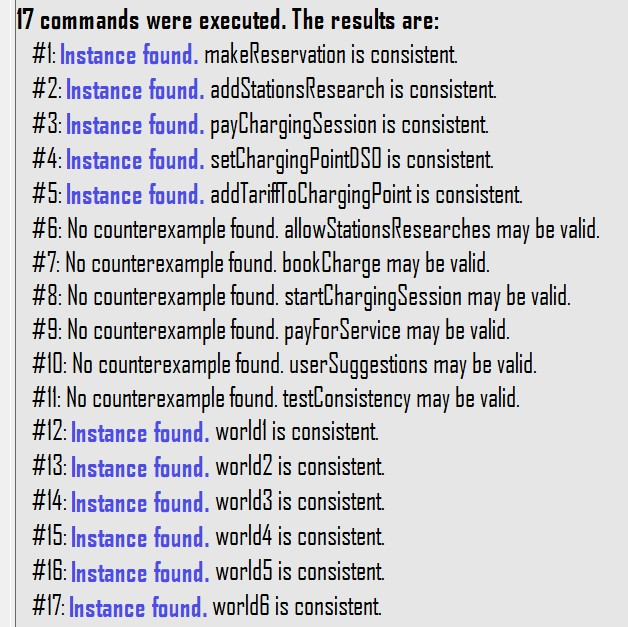
\includegraphics[width=0.5\textwidth]{Images/alloy/consistency.jpg}
    \caption{Result of the execution of "Execute all".}
    \label{fig:alloy-res-consistency}
\end{figure}

\newpage

\subsection{First world}

The first world (Figure~\ref{fig:world1}) gives a general view of the domain, where there are multiple Users and CPOs. Each CPO can own multiple Charging Points and each of them can have multiple Sockets.

\begin{figure}[H]
    \centering
    %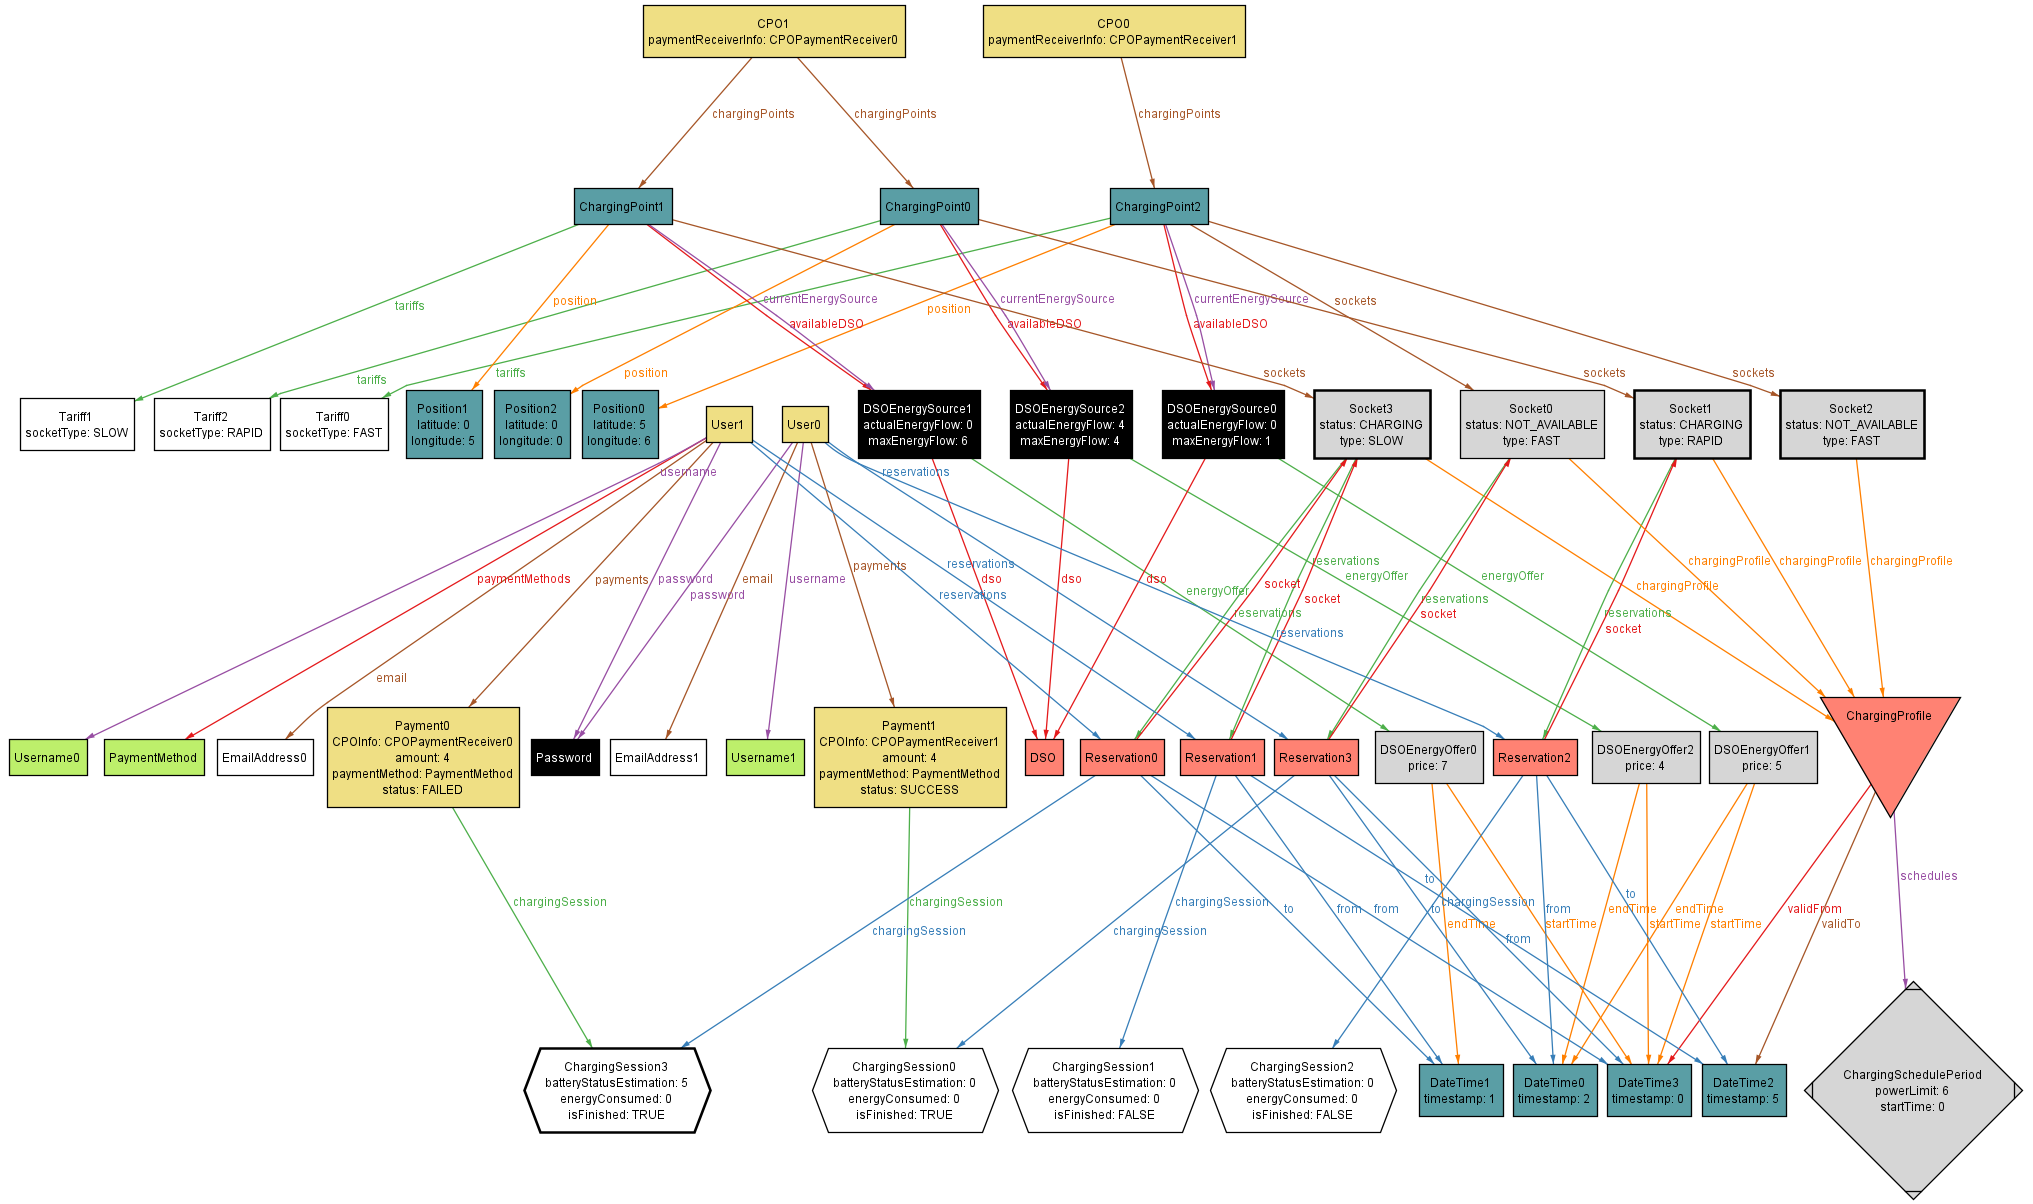
\includegraphics[angle=90,origin=c,height=0.95\textwidth]{Images/alloy/world1.png}
    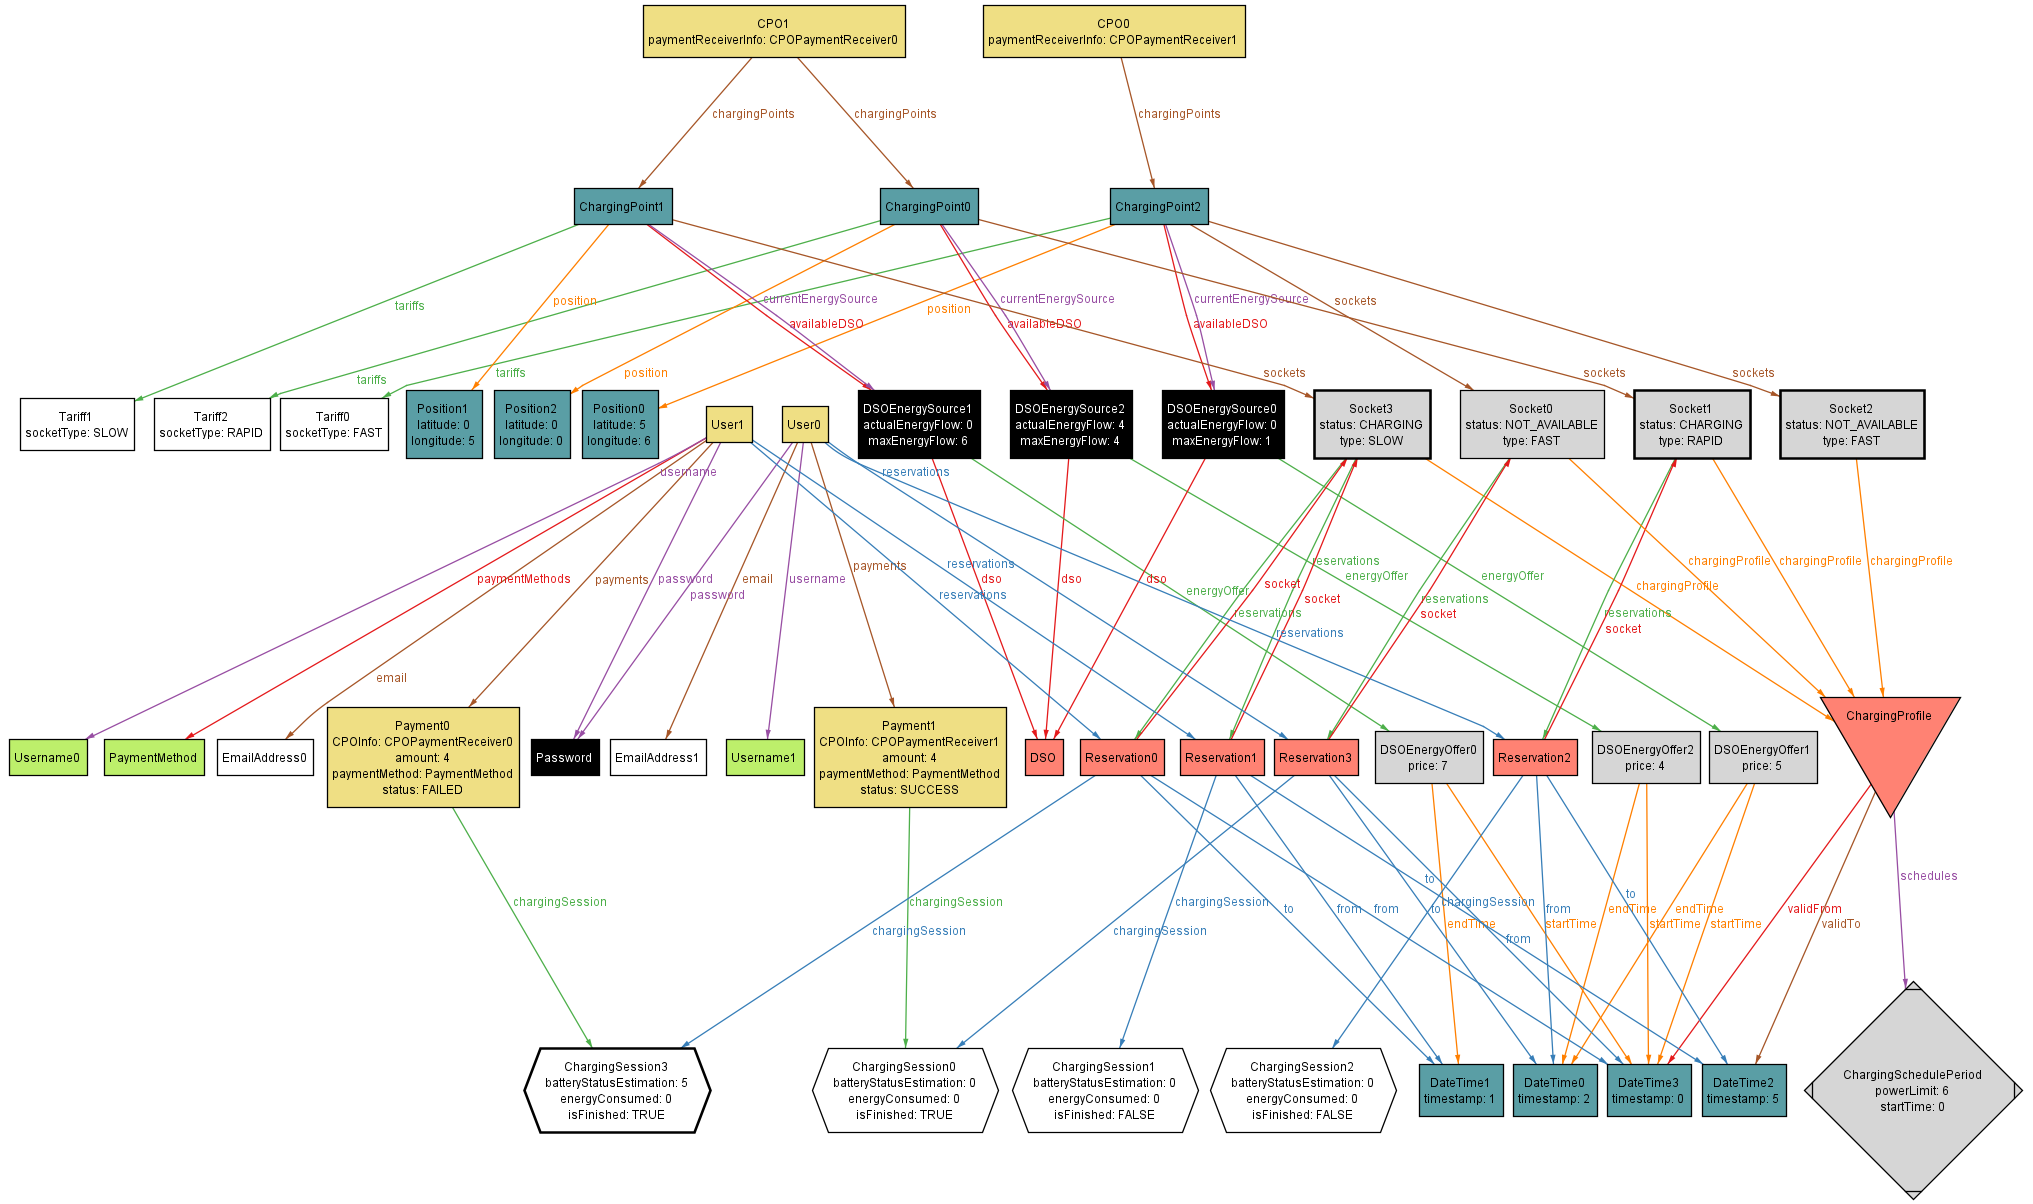
\includegraphics[width=1\textwidth]{Images/alloy/world1.png}
    \caption{World 1}
    \label{fig:world1}
\end{figure}

\subsection{Second world}

The second world (Figure~\ref{fig:world2}) is focused on \textbf{charging suggestions}. This model shows that a charging suggestion belongs only to a user and contains a suggested vehicle that is registered inside the vehicles of the user. Each charging suggestion is suggesting the user go and charge the suggested vehicle at a certain charging point. Each user cannot receive more than one suggestion at each time frame.

\begin{figure}[H]
    \centering
    %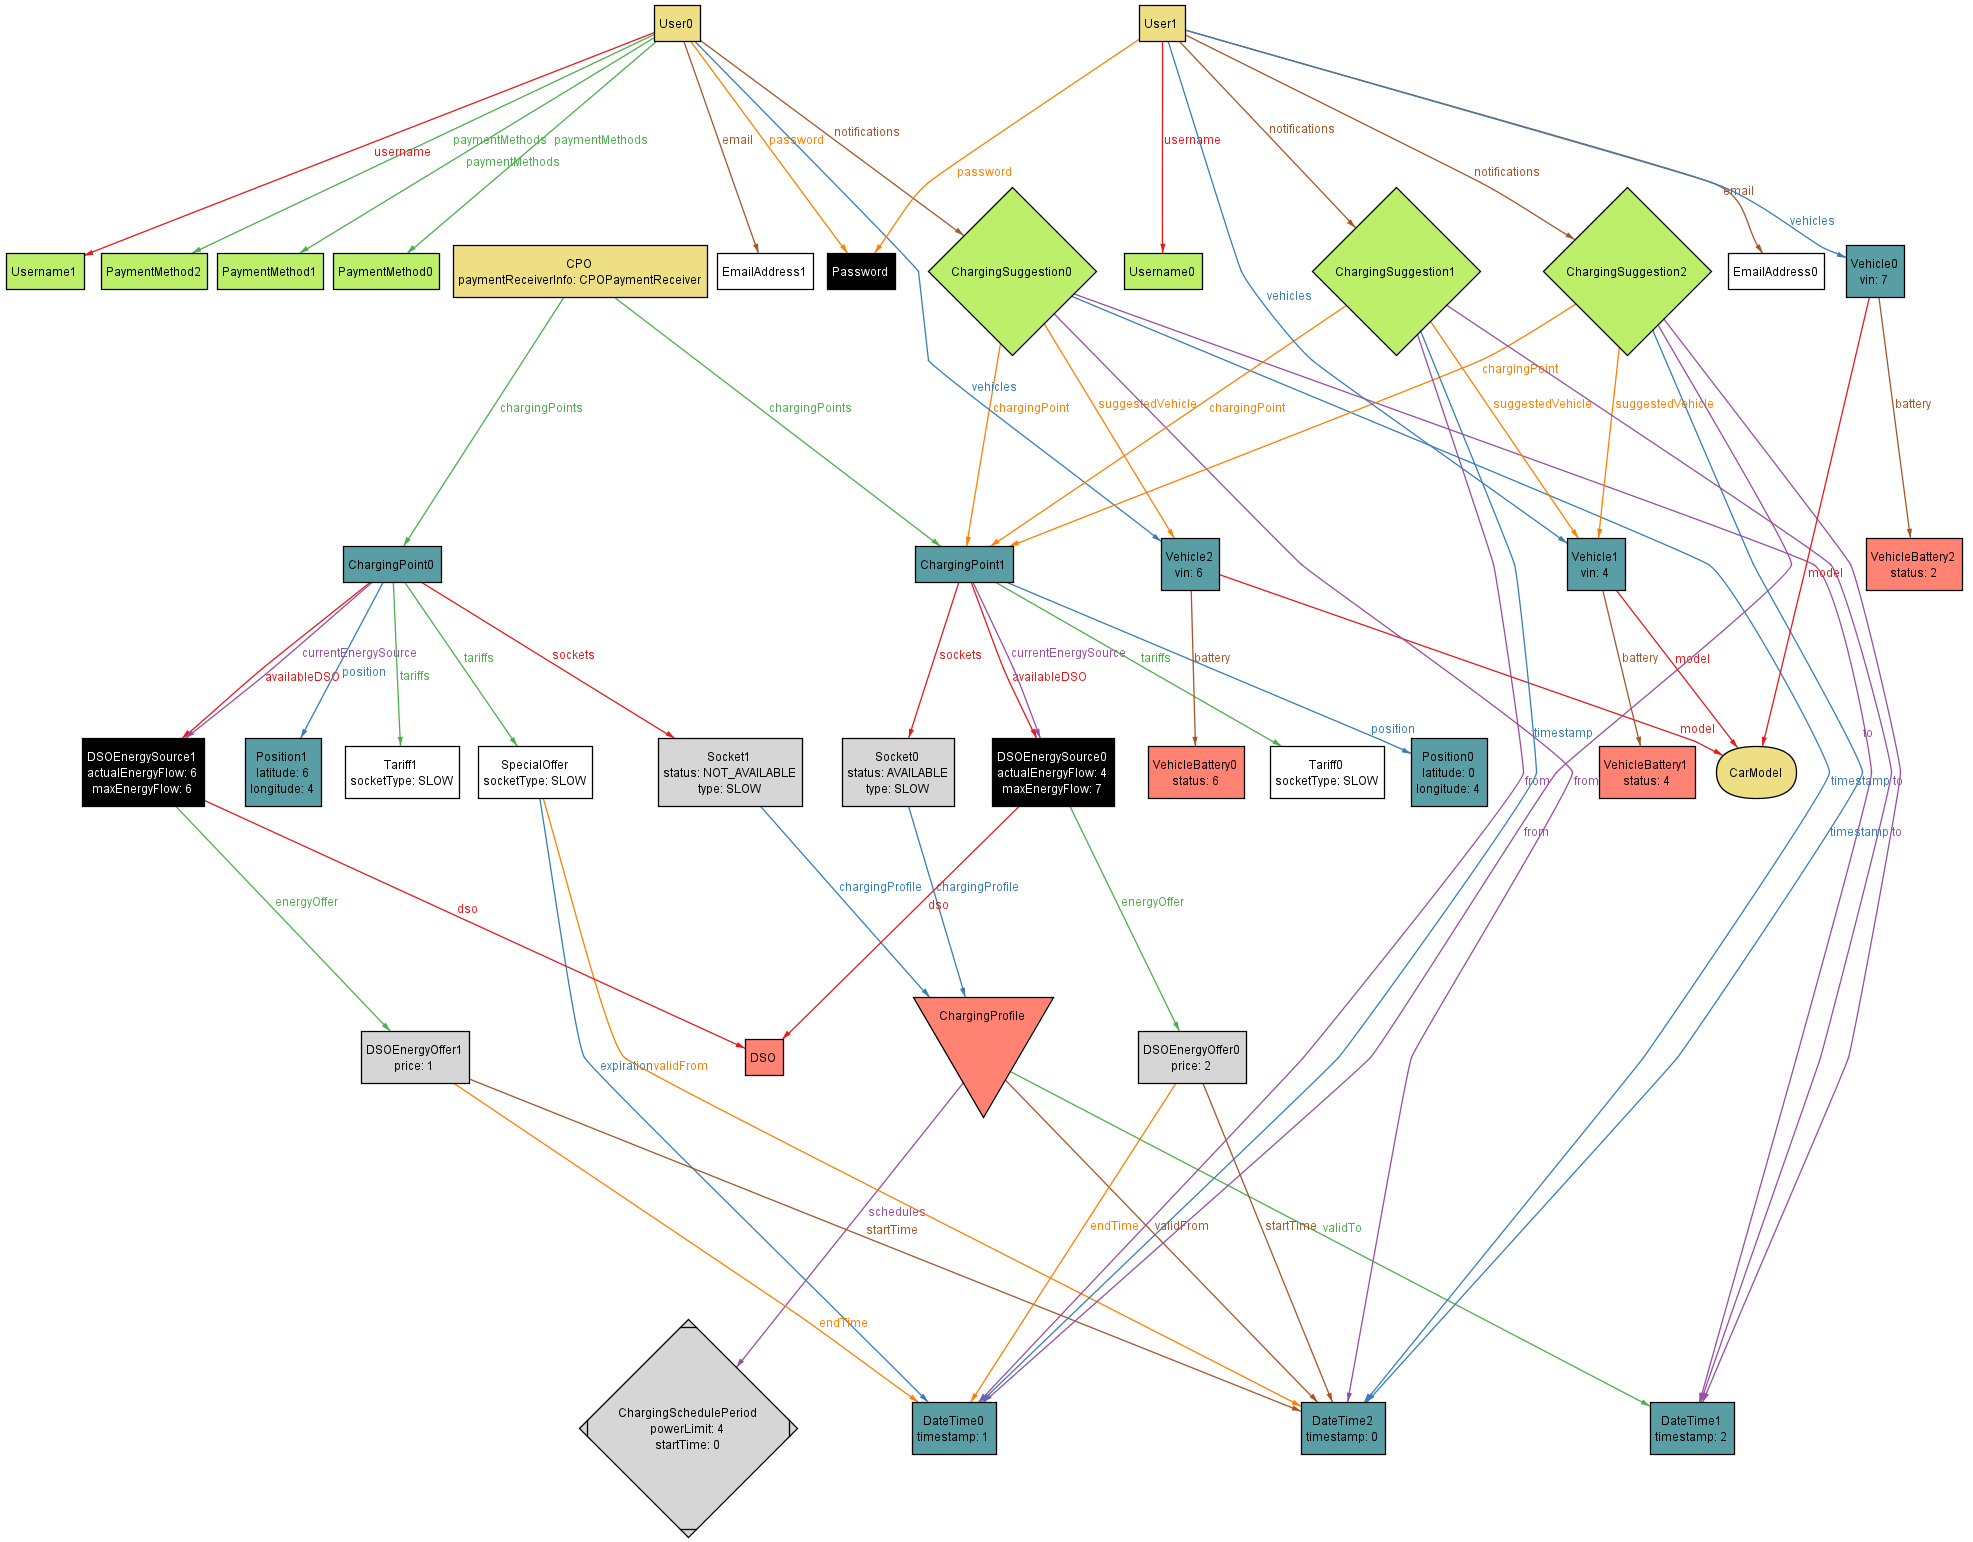
\includegraphics[angle=90,origin=c,height=0.95\textwidth]{Images/alloy/world2.png}
    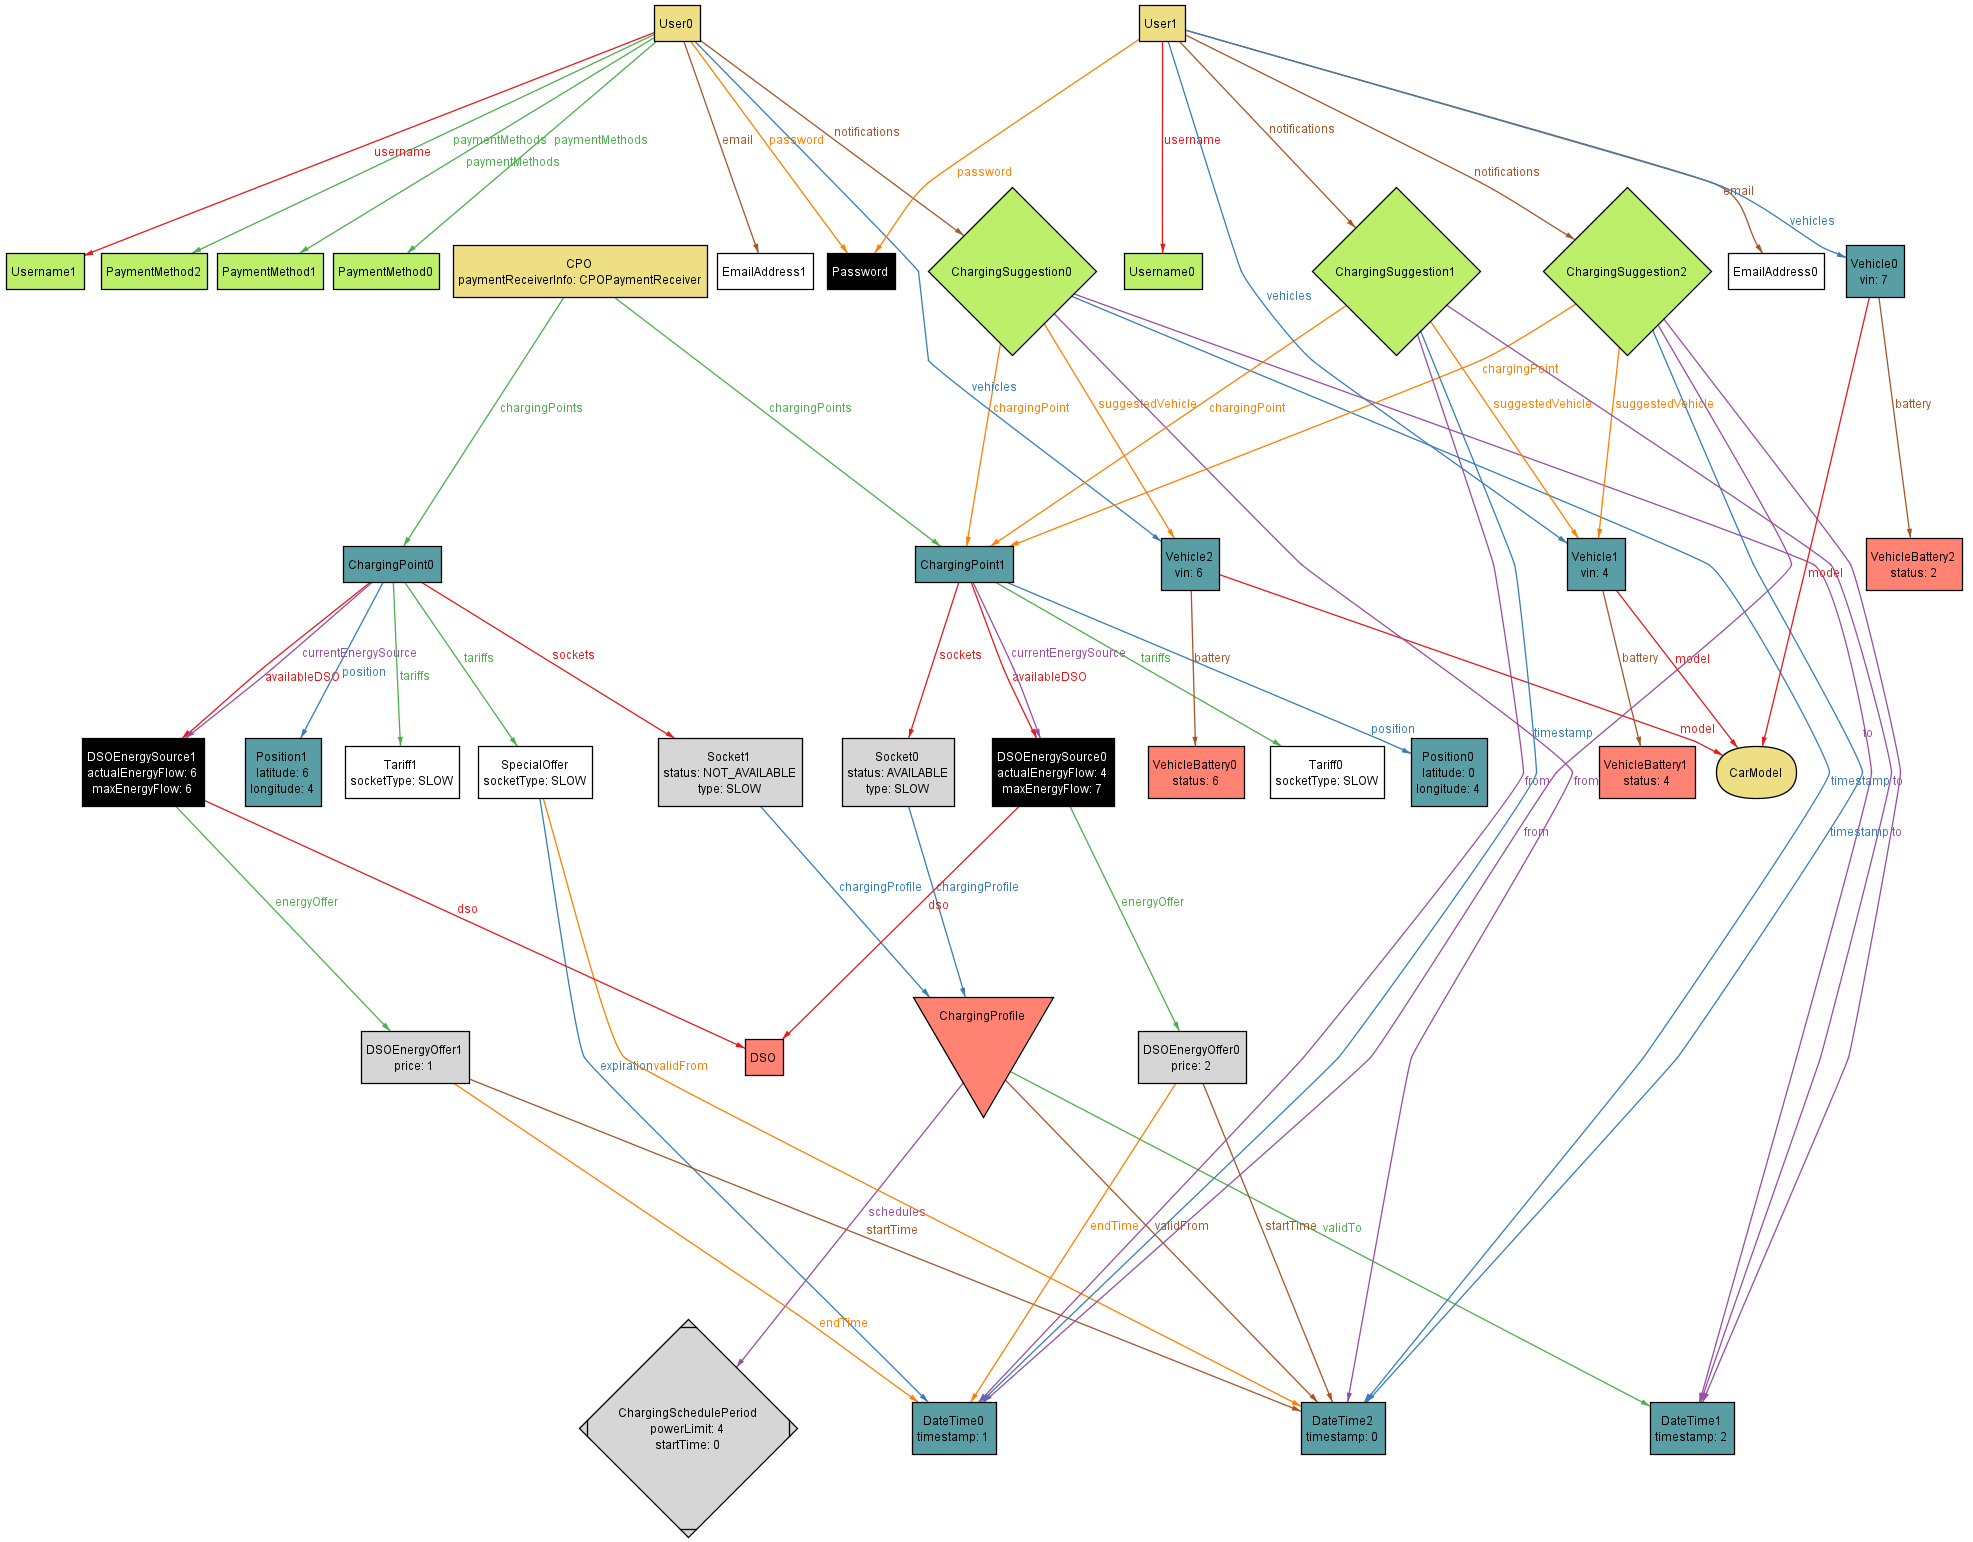
\includegraphics[width=1\textwidth]{Images/alloy/world2.png}
    \caption{World 2}
    \label{fig:world2}
\end{figure}

\subsection{Third world}

In the third world (Figure~\ref{fig:world3}) the focus is on the structure of a \textbf{charging point}. Each charging point can have multiple sockets of different types (SLOW, FAST, RAPID). If a certain charging point has at least a socket of a certain type, it must contain a tariff for that type of socket. A charging point can have also some special offers for some types of sockets, and these are valid for a certain period of time. Each charging point can be related to multiple energy sources, these can be batteries or can come from a DSO. Since a DSO can provide different offers for different CPOs (in terms of both the price and the maximum energy flow), each DSO has a different energy source for different CPOs. These energy sources contain also the history of all the offers that the DSO have made. The charging point can contain multiple current energy sources, but only one of those can be an energy source of a DSO.

\begin{figure}[H]
    \centering
    %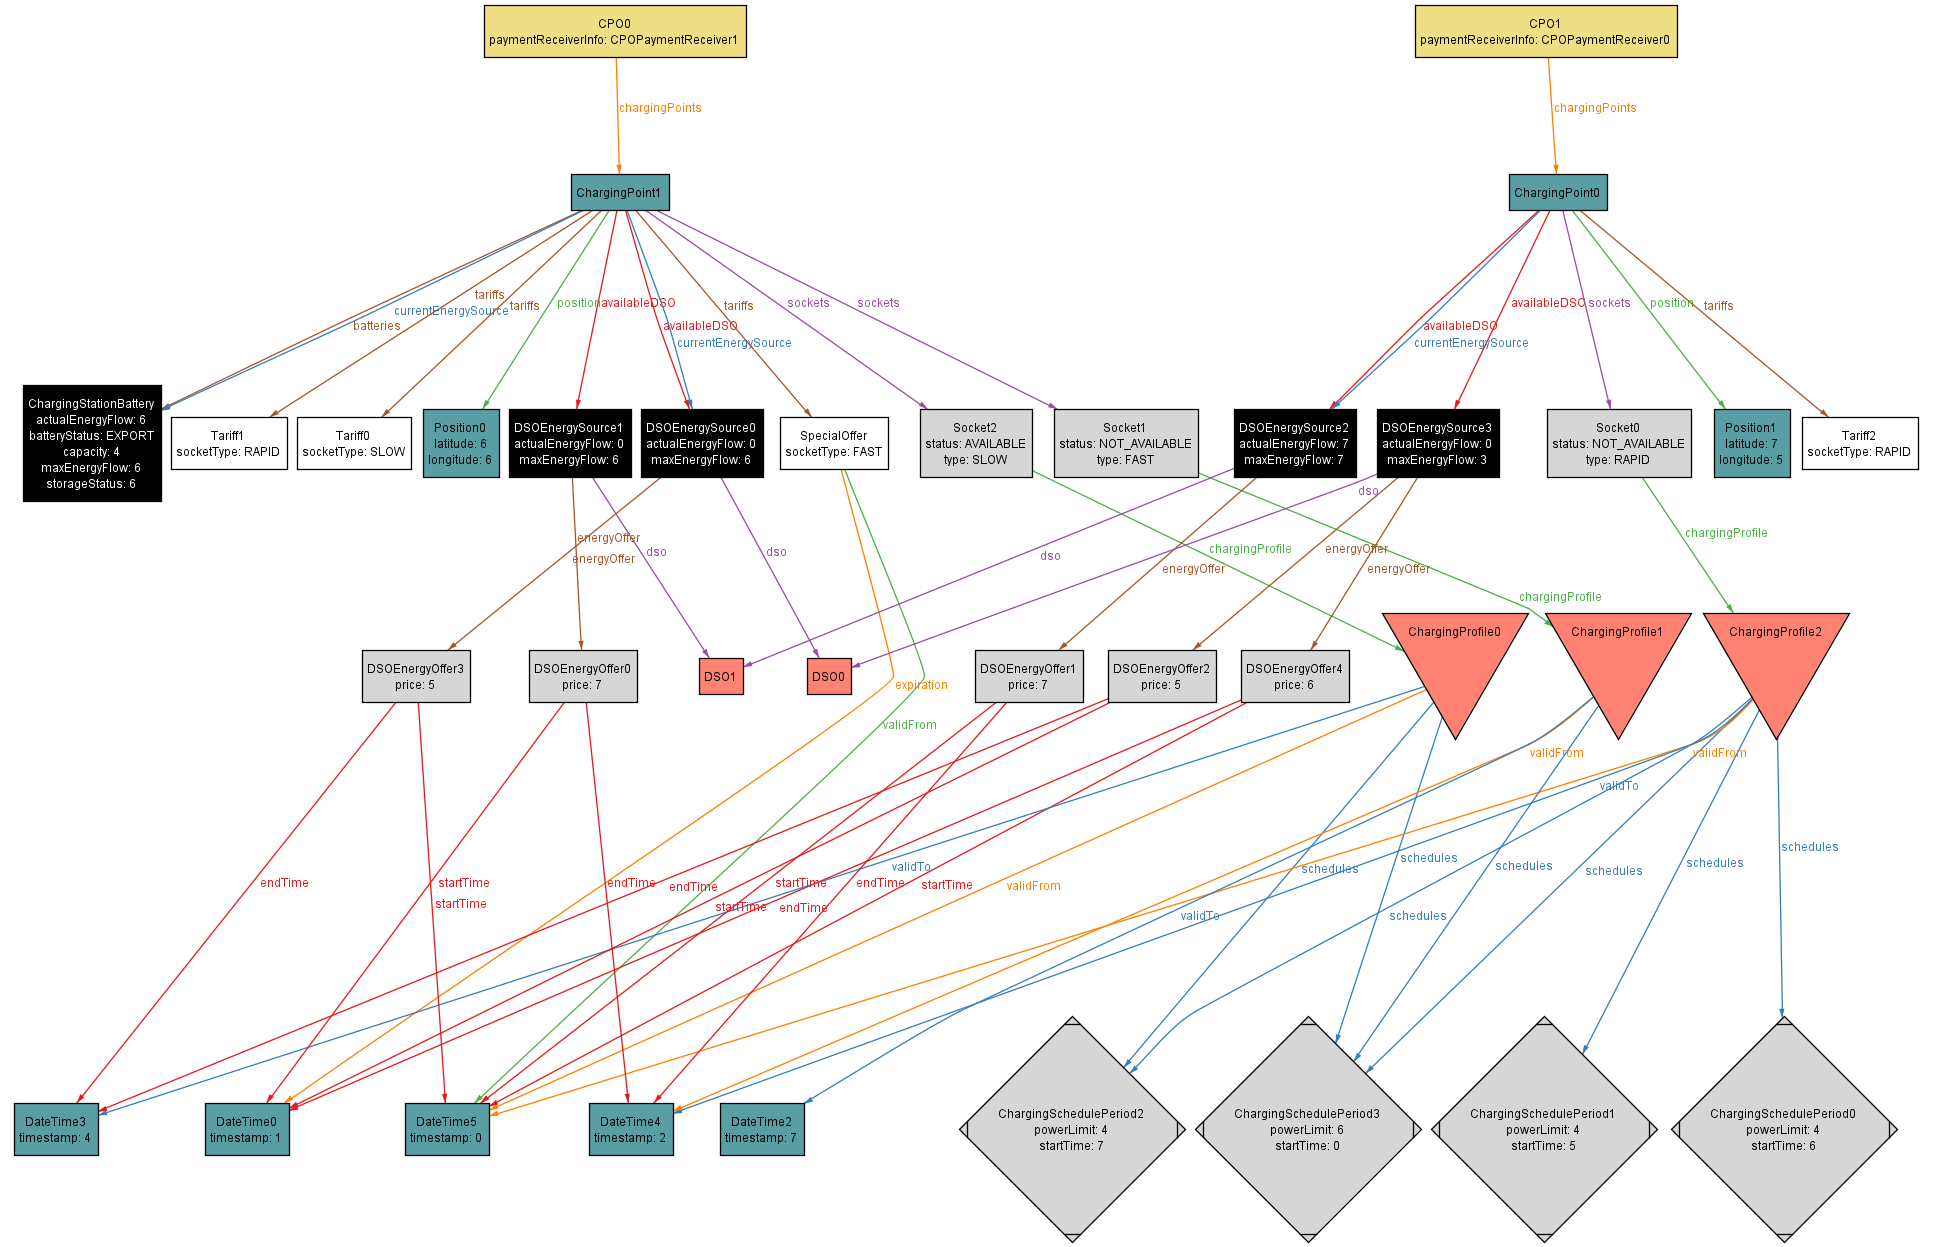
\includegraphics[angle=90,origin=c,height=0.95\textwidth]{Images/alloy/world3.png}
    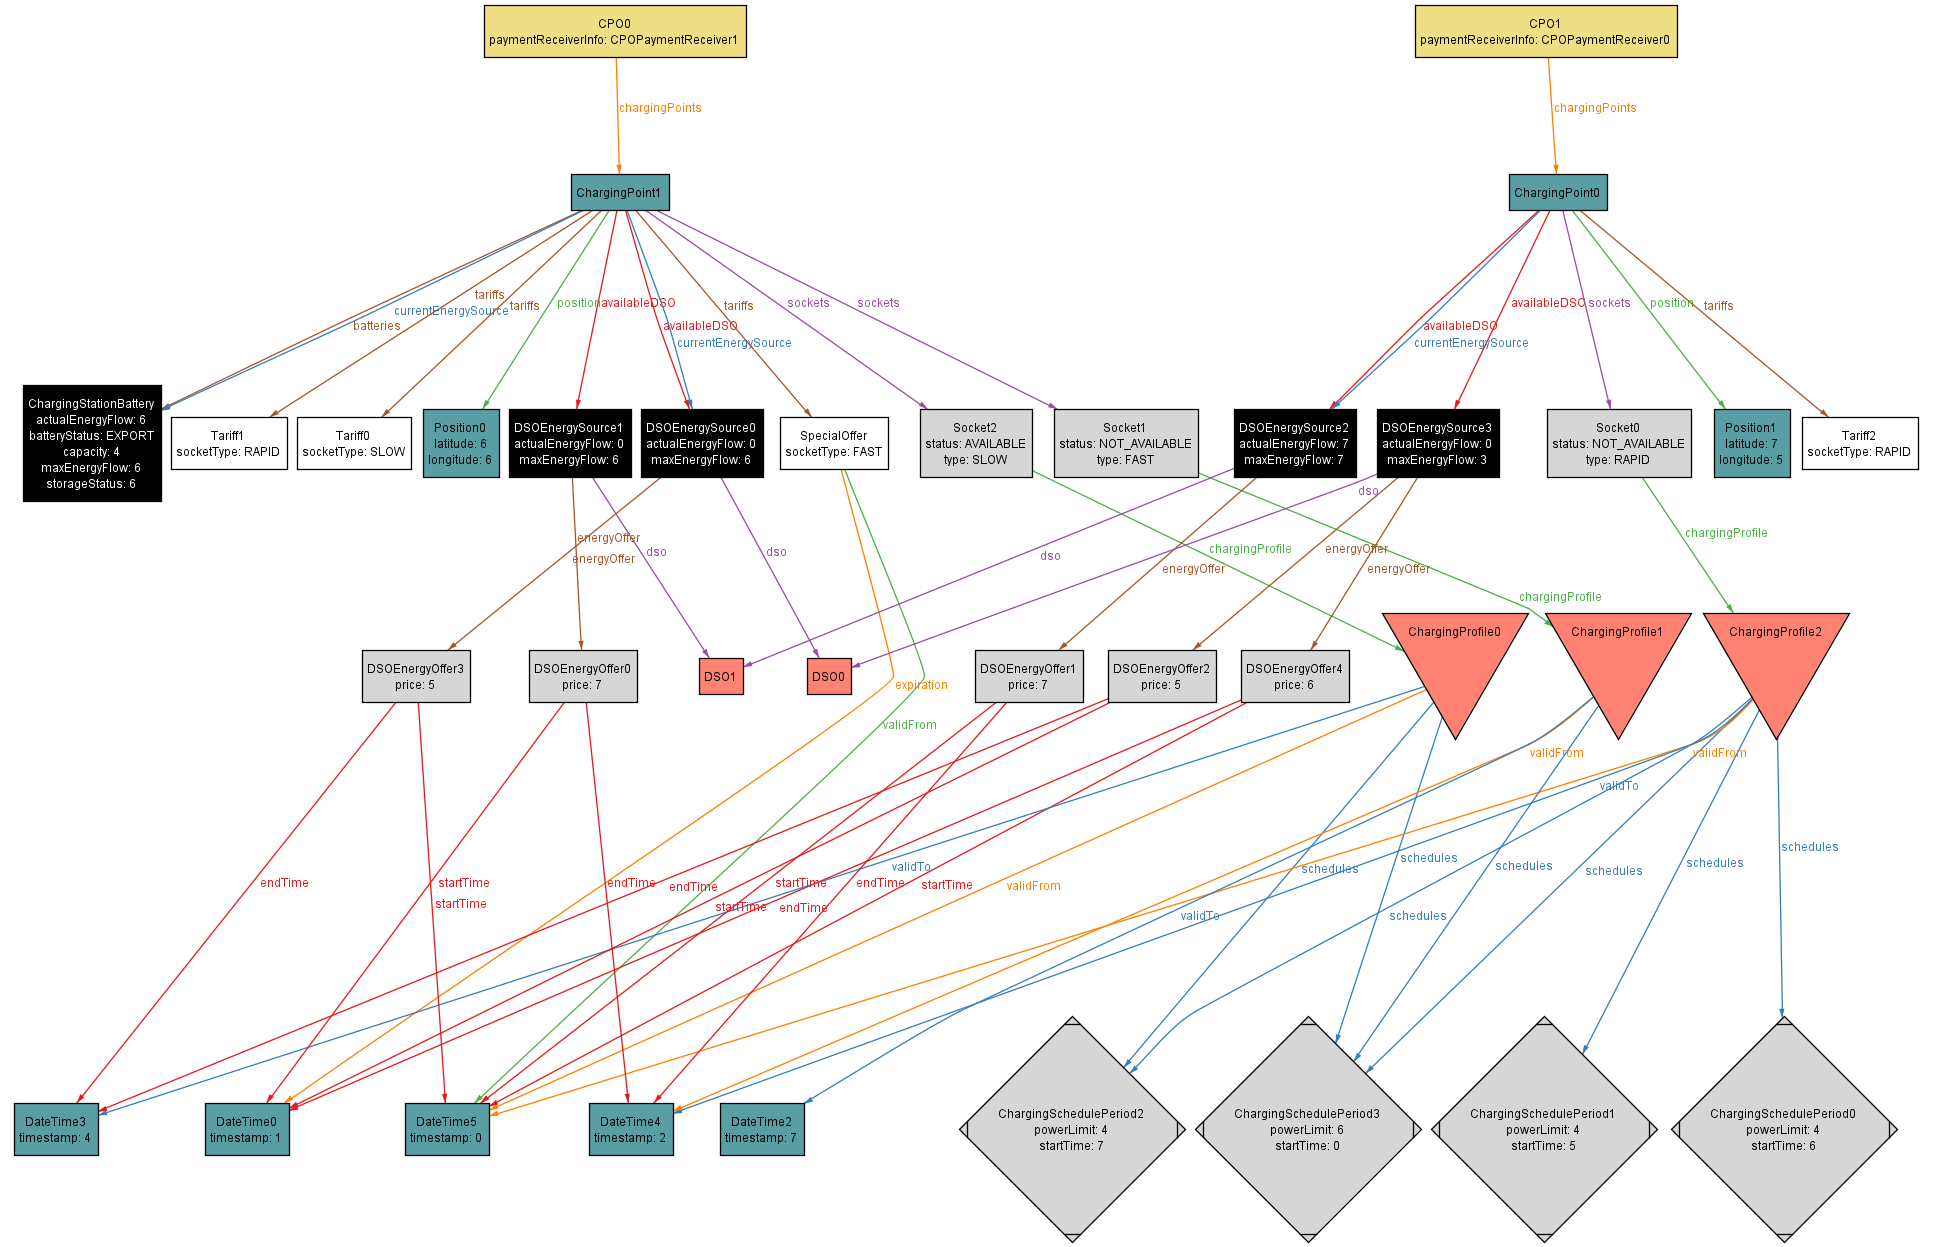
\includegraphics[width=1\textwidth]{Images/alloy/world3.png}
    \caption{World 3}
    \label{fig:world3}
\end{figure}

\subsection{Fourth world}

The fourth world (Figure~\ref{fig:world4}) is concentrated on the users' data. Each \textbf{user} can register some vehicles and each vehicle can be registered by more than one user.

\begin{figure}[H]
    \centering
    %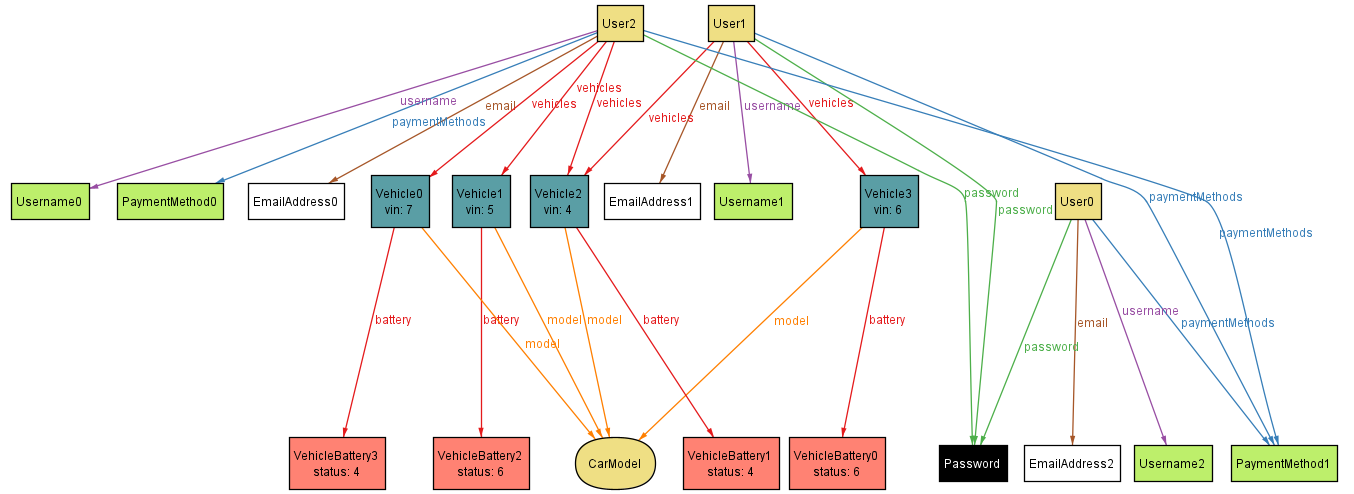
\includegraphics[angle=90,origin=c,height=0.95\textwidth]{Images/alloy/world4.png}
    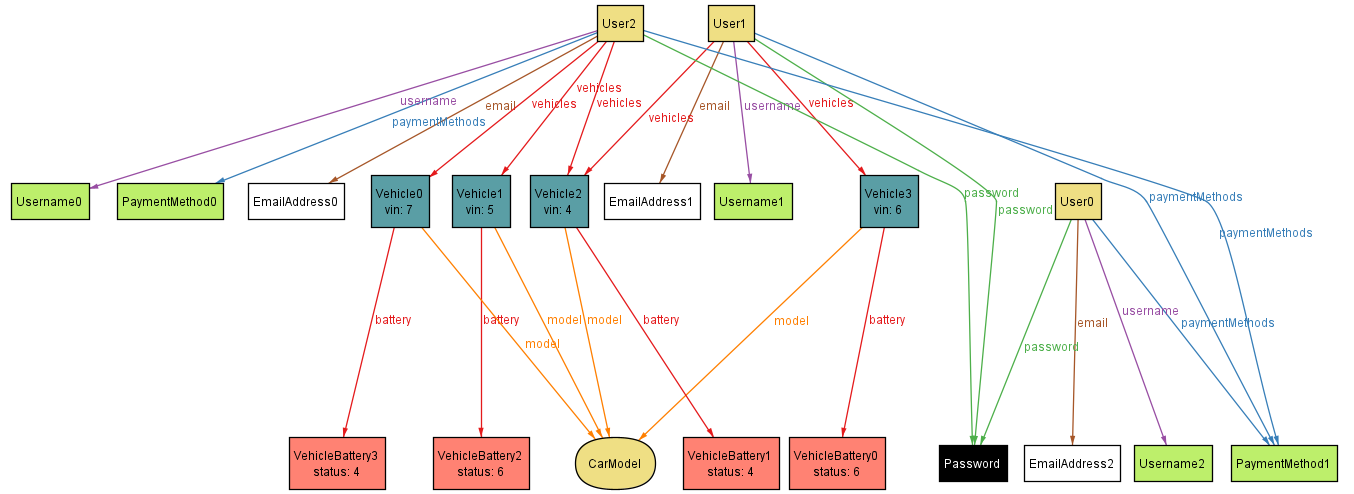
\includegraphics[width=1\textwidth]{Images/alloy/world4.png}
    \caption{World 4}
    \label{fig:world4}
\end{figure}

\subsection{Fifth world}

The fifth world (Figure~\ref{fig:world5}) is focused on the \textbf{registrations} on the same socket. Two registrations cannot overlap if they are related to the same socket. Each user can make a reservation only if he doesn't have any pending payments (i.e. if all the payments have SUCCESS as a status) and only his last reservation can be active (i.e. with a not started or not finished charging session).

\begin{figure}[H]
    \centering
    %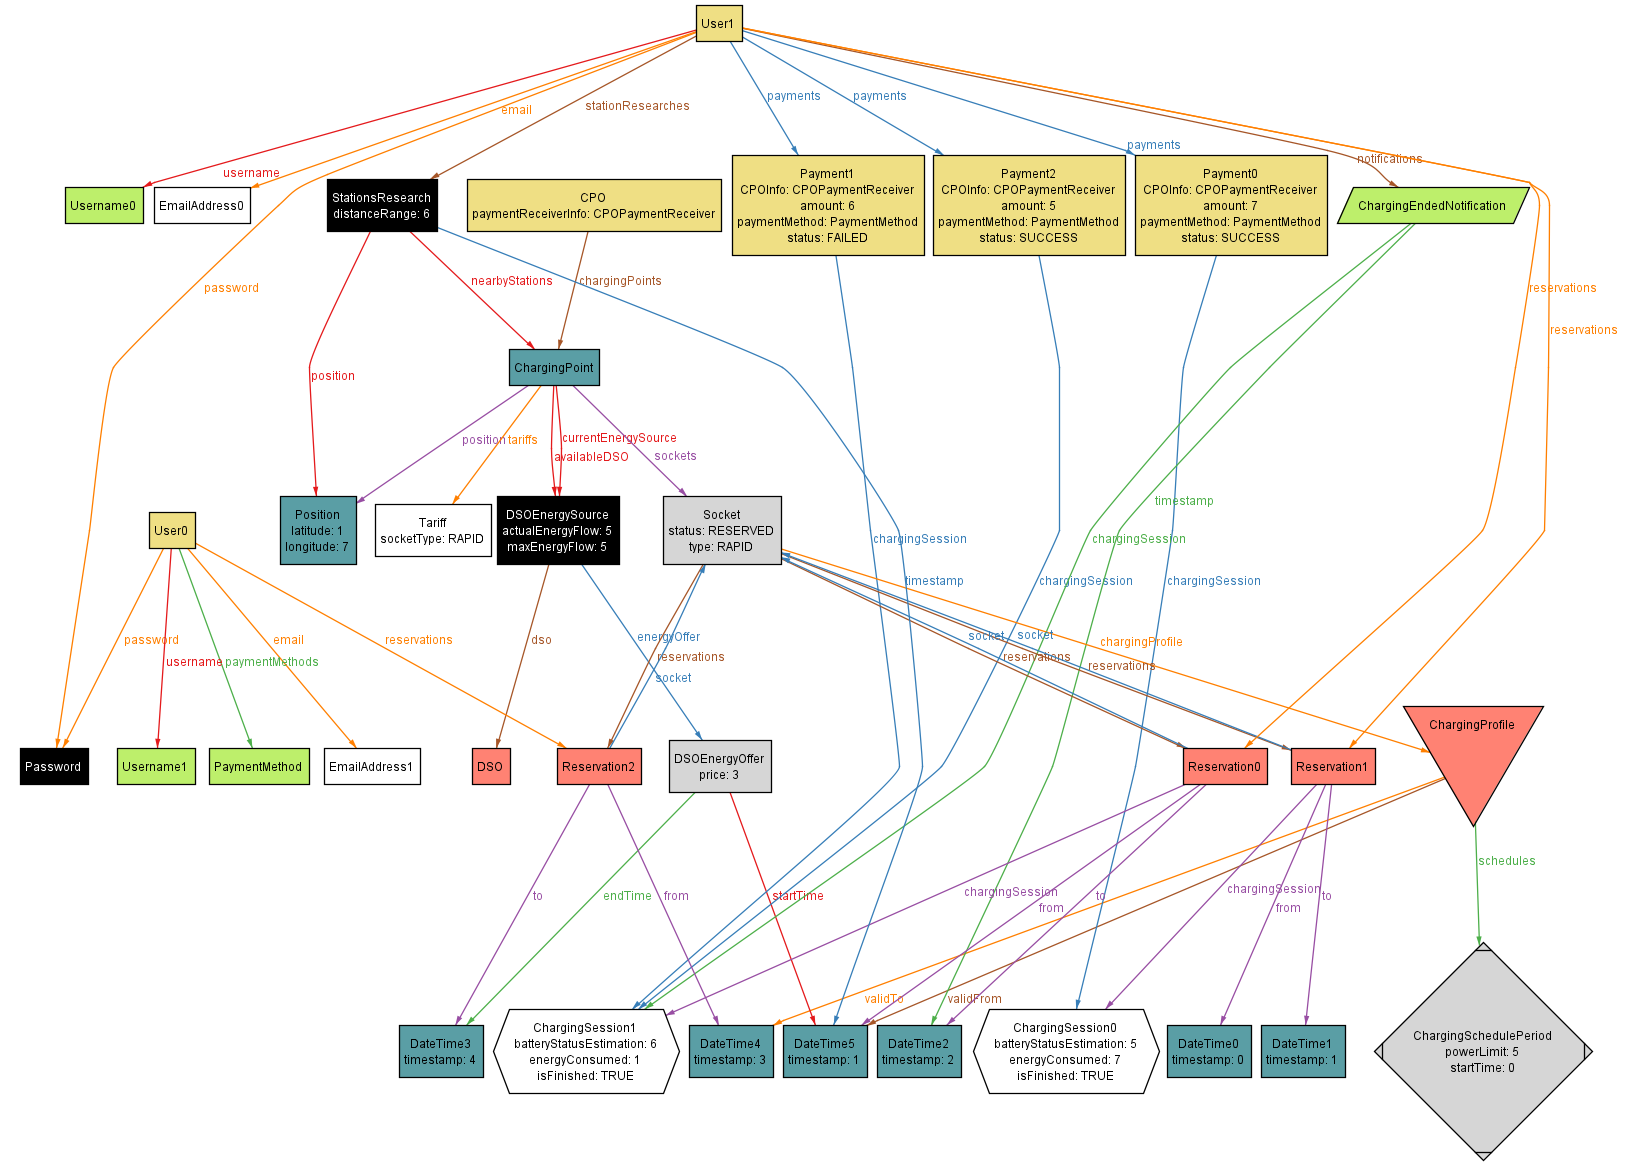
\includegraphics[angle=90,origin=c,height=0.95\textwidth]{Images/alloy/world5.png}
    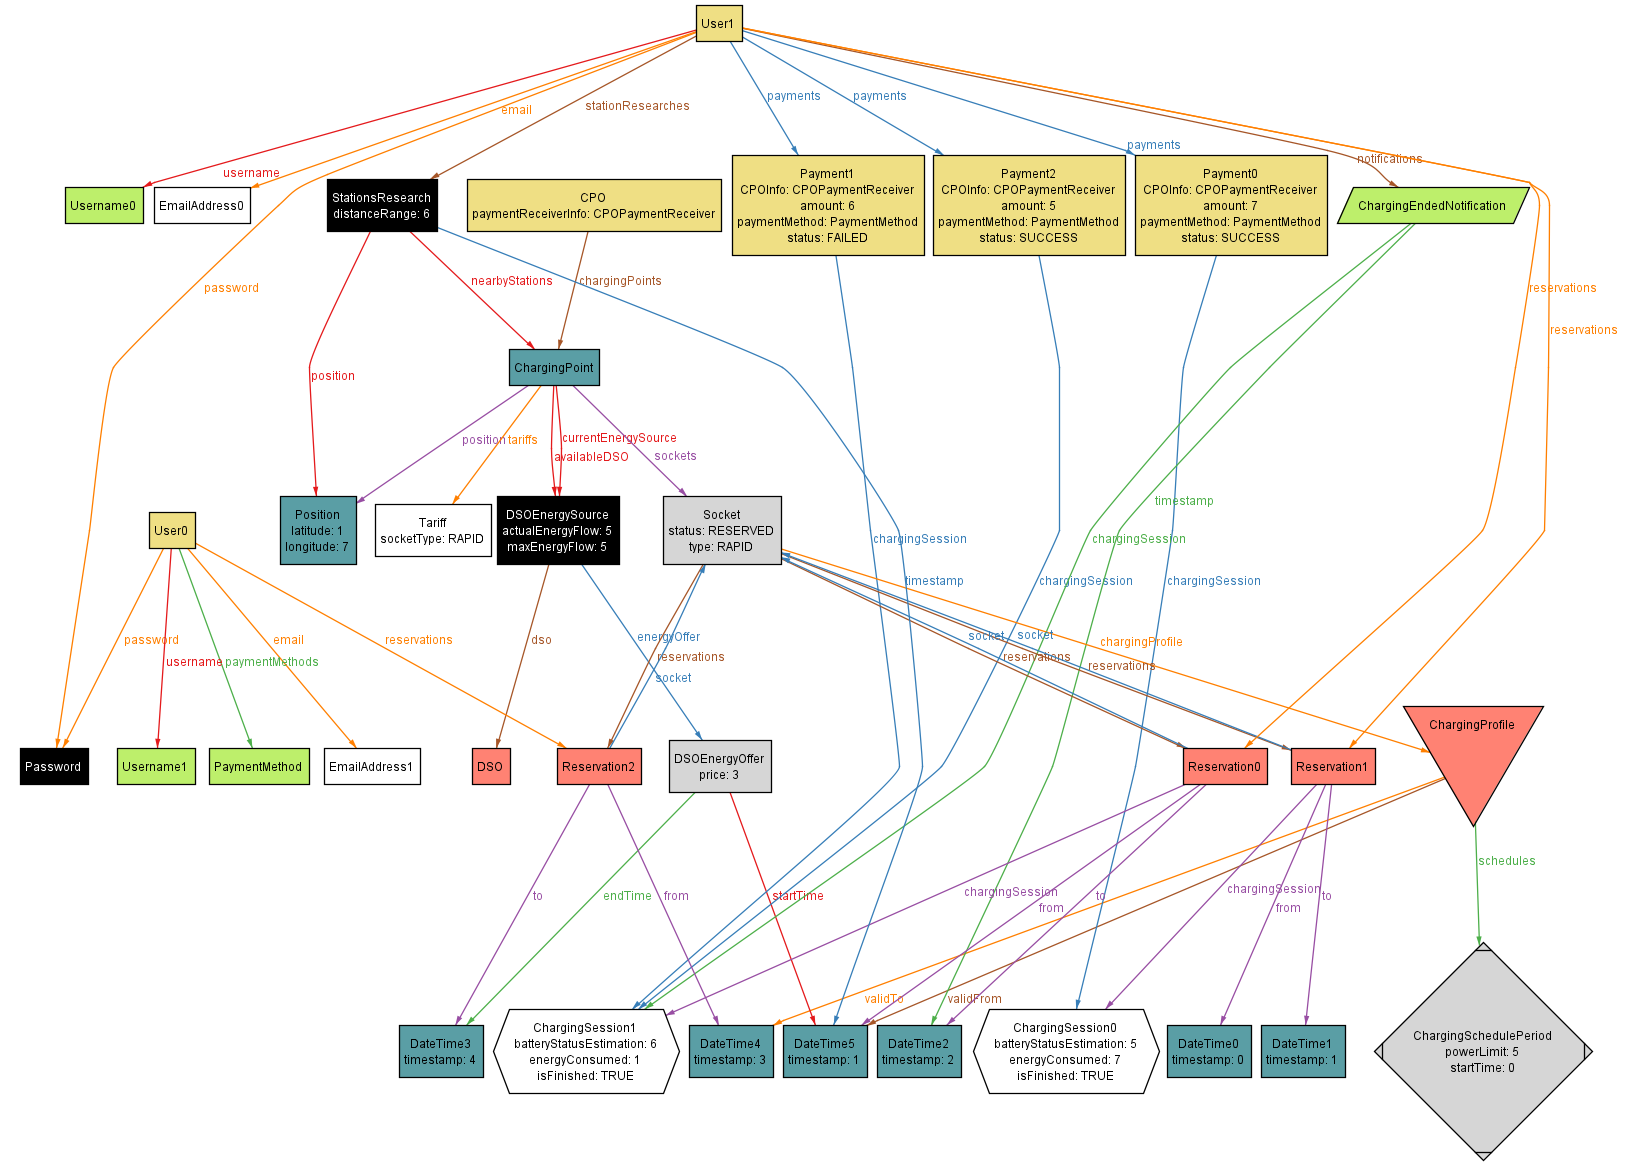
\includegraphics[width=1\textwidth]{Images/alloy/world5.png}
    \caption{World 5}
    \label{fig:world5}
\end{figure}

\subsection{Sixth world}

In the sixth world (Figure~\ref{fig:world6}) the focus is on the \textbf{stations researches}. A user is connected to some stations' research; each of those has a position around which the research is made and a distance range. All charging points that are inside the distance range are returned.

\begin{figure}[H]
    \centering
    %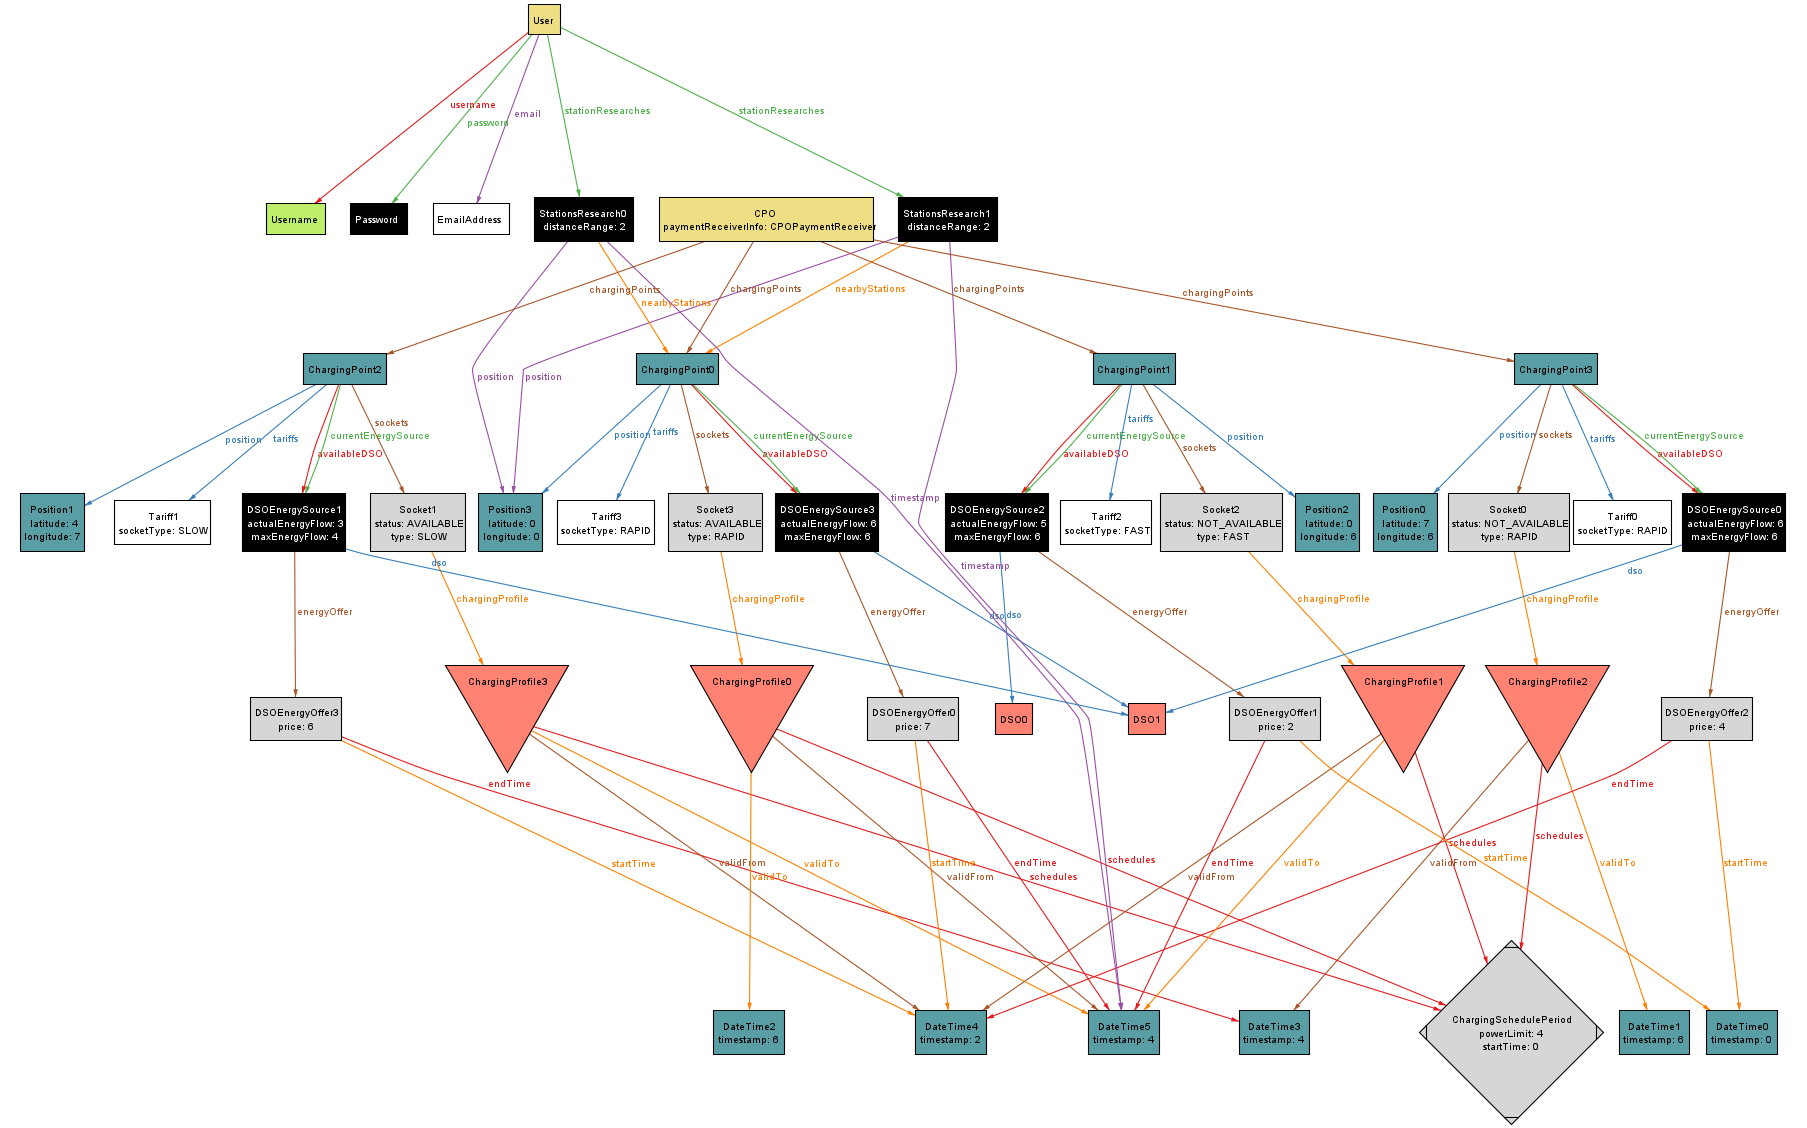
\includegraphics[angle=90,origin=c,height=0.95\textwidth]{Images/alloy/world6.png}
    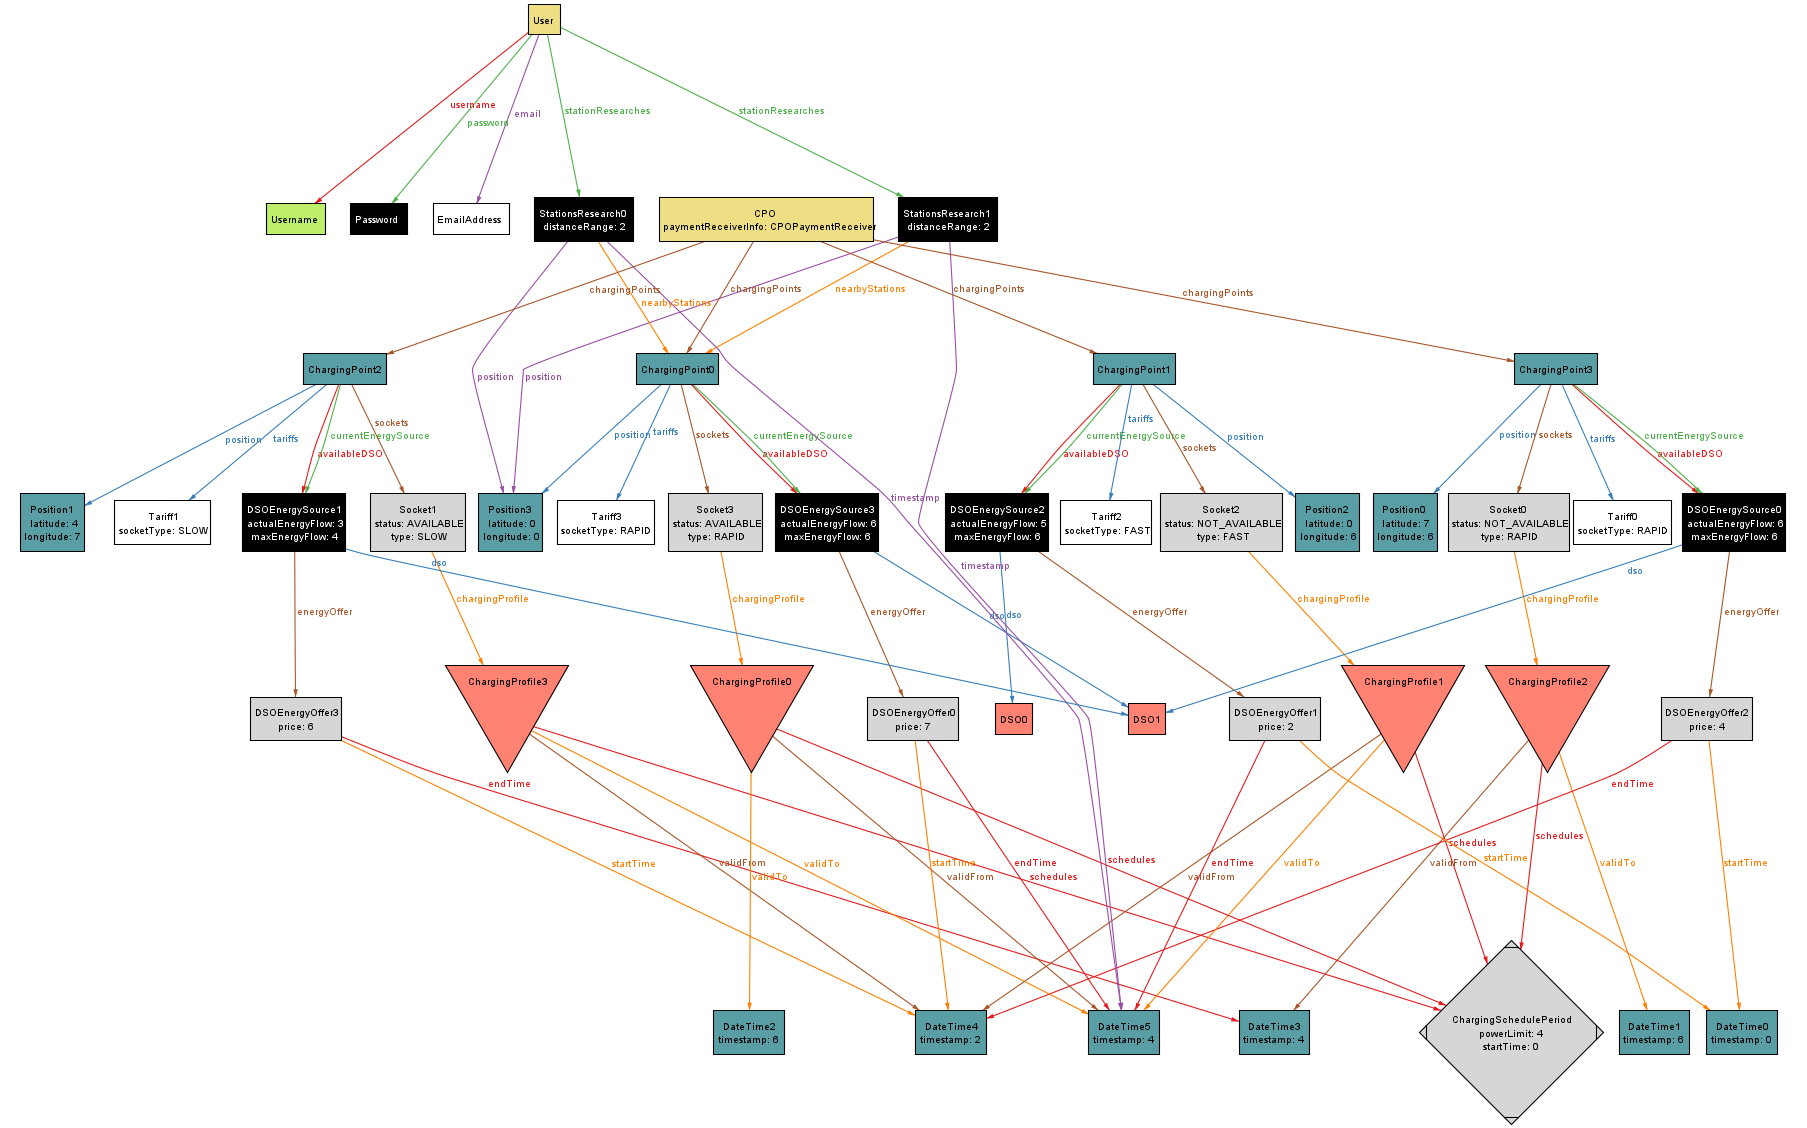
\includegraphics[width=1\textwidth]{Images/alloy/world6.png}
    \caption{World 6}
    \label{fig:world6}
\end{figure}

\chapter{Effort Spent}

\section{Lorenzo Ferretti}

\begin{table}[H]
    \centering 
    \begin{tabular}{|l|c|}
    \hline
    \rowcolor{bluepoli!40}
    \textbf{Task} & \textbf{Hours Spent} \T\B \\
    \hline
    Introduction & 5 \T\B \\
    \hline
    Overall Description & 20 \T\B \\
    \hline
    Specific Requirements & 25\T\B \\
    \hline
    Formal Analysis & 5 \T\B \\
    \hline
    \end{tabular}
\end{table}

\section{Lorenzo Manoni}

\begin{table}[H]
    \centering 
    \begin{tabular}{|l|c|}
    \hline
    \rowcolor{bluepoli!40}
    \textbf{Task} & \textbf{Hours Spent} \T\B \\
    \hline
    Introduction & 10\T\B \\
    \hline
    Overall Description & 15\T\B \\
    \hline
    Specific Requirements & 25\T\B \\
    \hline
    Formal Analysis & 5\T\B \\
    \hline
    \end{tabular}
\end{table}

\section{Carlo Sgaravatti}

\begin{table}[H]
    \centering 
    \begin{tabular}{|l|c|}
    \hline
    \rowcolor{bluepoli!40}
    \textbf{Task} & \textbf{Hours Spent} \T\B \\
    \hline
    Introduction & 8\T\B \\
    \hline
    Overall Description & 10\T\B \\
    \hline
    Specific Requirements & 15\T\B \\
    \hline
    Formal Analysis & 22\T\B \\
    \hline
    \end{tabular}
\end{table}

%-------------------------------------------------------------------------
%	APPENDICES
%-------------------------------------------------------------------------

\cleardoublepage
\addtocontents{toc}{\vspace{2em}} % Add a gap in the Contents, for aesthetics
%\appendix
%\chapter{Appendix A}
%If you need to include an appendix to support the research in your thesis, you can place it at the end of the manuscript.
%An appendix contains supplementary material (figures, tables, data, codes, mathematical proofs, surveys, \dots)
%which supplement the main results contained in the previous chapters.


\cleardoublepage

\end{document}
